\documentclass[twoside]{book}

% Packages required by doxygen
\usepackage{fixltx2e}
\usepackage{calc}
\usepackage{doxygen}
\usepackage[export]{adjustbox} % also loads graphicx
\usepackage{graphicx}
\usepackage[utf8]{inputenc}
\usepackage{makeidx}
\usepackage{multicol}
\usepackage{multirow}
\PassOptionsToPackage{warn}{textcomp}
\usepackage{textcomp}
\usepackage[nointegrals]{wasysym}
\usepackage[table]{xcolor}

% Font selection
\usepackage[T1]{fontenc}
\usepackage[scaled=.90]{helvet}
\usepackage{courier}
\usepackage{amssymb}
\usepackage{sectsty}
\renewcommand{\familydefault}{\sfdefault}
\allsectionsfont{%
  \fontseries{bc}\selectfont%
  \color{darkgray}%
}
\renewcommand{\DoxyLabelFont}{%
  \fontseries{bc}\selectfont%
  \color{darkgray}%
}
\newcommand{\+}{\discretionary{\mbox{\scriptsize$\hookleftarrow$}}{}{}}

% Page & text layout
\usepackage{geometry}
\geometry{%
  a4paper,%
  top=2.5cm,%
  bottom=2.5cm,%
  left=2.5cm,%
  right=2.5cm%
}
\tolerance=750
\hfuzz=15pt
\hbadness=750
\setlength{\emergencystretch}{15pt}
\setlength{\parindent}{0cm}
\setlength{\parskip}{3ex plus 2ex minus 2ex}
\makeatletter
\renewcommand{\paragraph}{%
  \@startsection{paragraph}{4}{0ex}{-1.0ex}{1.0ex}{%
    \normalfont\normalsize\bfseries\SS@parafont%
  }%
}
\renewcommand{\subparagraph}{%
  \@startsection{subparagraph}{5}{0ex}{-1.0ex}{1.0ex}{%
    \normalfont\normalsize\bfseries\SS@subparafont%
  }%
}
\makeatother

% Headers & footers
\usepackage{fancyhdr}
\pagestyle{fancyplain}
\fancyhead[LE]{\fancyplain{}{\bfseries\thepage}}
\fancyhead[CE]{\fancyplain{}{}}
\fancyhead[RE]{\fancyplain{}{\bfseries\leftmark}}
\fancyhead[LO]{\fancyplain{}{\bfseries\rightmark}}
\fancyhead[CO]{\fancyplain{}{}}
\fancyhead[RO]{\fancyplain{}{\bfseries\thepage}}
\fancyfoot[LE]{\fancyplain{}{}}
\fancyfoot[CE]{\fancyplain{}{}}
\fancyfoot[RE]{\fancyplain{}{\bfseries\scriptsize Generated by Doxygen }}
\fancyfoot[LO]{\fancyplain{}{\bfseries\scriptsize Generated by Doxygen }}
\fancyfoot[CO]{\fancyplain{}{}}
\fancyfoot[RO]{\fancyplain{}{}}
\renewcommand{\footrulewidth}{0.4pt}
\renewcommand{\chaptermark}[1]{%
  \markboth{#1}{}%
}
\renewcommand{\sectionmark}[1]{%
  \markright{\thesection\ #1}%
}

% Indices & bibliography
\usepackage{natbib}
\usepackage[titles]{tocloft}
\setcounter{tocdepth}{3}
\setcounter{secnumdepth}{5}
\makeindex

% Hyperlinks (required, but should be loaded last)
\usepackage{ifpdf}
\ifpdf
  \usepackage[pdftex,pagebackref=true]{hyperref}
\else
  \usepackage[ps2pdf,pagebackref=true]{hyperref}
\fi
\hypersetup{%
  colorlinks=true,%
  linkcolor=blue,%
  citecolor=blue,%
  unicode%
}

% Custom commands
\newcommand{\clearemptydoublepage}{%
  \newpage{\pagestyle{empty}\cleardoublepage}%
}

\usepackage{caption}
\captionsetup{labelsep=space,justification=centering,font={bf},singlelinecheck=off,skip=4pt,position=top}

%===== C O N T E N T S =====

\begin{document}

% Titlepage & ToC
\hypersetup{pageanchor=false,
             bookmarksnumbered=true,
             pdfencoding=unicode
            }
\pagenumbering{alph}
\begin{titlepage}
\vspace*{7cm}
\begin{center}%
{\Large Bigfoot\+DS Unity Tools \\[1ex]\large 1 }\\
\vspace*{1cm}
{\large Generated by Doxygen 1.8.14}\\
\end{center}
\end{titlepage}
\clearemptydoublepage
\pagenumbering{roman}
\tableofcontents
\clearemptydoublepage
\pagenumbering{arabic}
\hypersetup{pageanchor=true}

%--- Begin generated contents ---
\chapter{Namespace Index}
\section{Packages}
Here are the packages with brief descriptions (if available)\+:\begin{DoxyCompactList}
\item\contentsline{section}{\mbox{\hyperlink{namespace_bigfoot_d_s}{Bigfoot\+DS}} }{\pageref{namespace_bigfoot_d_s}}{}
\end{DoxyCompactList}

\chapter{Hierarchical Index}
\section{Class Hierarchy}
This inheritance list is sorted roughly, but not completely, alphabetically\+:\begin{DoxyCompactList}
\item \contentsline{section}{Bigfoot\+D\+S.\+Bigfoot\+Dice\+And\+Coins}{\pageref{class_bigfoot_d_s_1_1_bigfoot_dice_and_coins}}{}
\item Editor\+Window\begin{DoxyCompactList}
\item \contentsline{section}{Bigfoot\+D\+S.\+Scene\+Basics\+Generator}{\pageref{class_bigfoot_d_s_1_1_scene_basics_generator}}{}
\end{DoxyCompactList}
\item Mono\+Behaviour\begin{DoxyCompactList}
\item \contentsline{section}{Bigfoot\+D\+S.\+Bigfoot\+Dummy\+Test\+Script}{\pageref{class_bigfoot_d_s_1_1_bigfoot_dummy_test_script}}{}
\item \contentsline{section}{Bigfoot\+D\+S.\+Bigfoot\+Event\+Invoker}{\pageref{class_bigfoot_d_s_1_1_bigfoot_event_invoker}}{}
\item \contentsline{section}{Bigfoot\+D\+S.\+Bigfoot\+General\+Location\+Finder}{\pageref{class_bigfoot_d_s_1_1_bigfoot_general_location_finder}}{}
\item \contentsline{section}{Bigfoot\+D\+S.\+Bigfoot\+Normals\+Inverter}{\pageref{class_bigfoot_d_s_1_1_bigfoot_normals_inverter}}{}
\item \contentsline{section}{Bigfoot\+D\+S.\+Colour\+Changer\+Tester}{\pageref{class_bigfoot_d_s_1_1_colour_changer_tester}}{}
\item \contentsline{section}{Bigfoot\+D\+S.\+Folder\+Structure\+Generator}{\pageref{class_bigfoot_d_s_1_1_folder_structure_generator}}{}
\item \contentsline{section}{Bigfoot\+D\+S.\+Scene\+Changing}{\pageref{class_bigfoot_d_s_1_1_scene_changing}}{}
\item \contentsline{section}{Bigfoot\+D\+S.\+Simple\+Point\+To\+Point\+Mover}{\pageref{class_bigfoot_d_s_1_1_simple_point_to_point_mover}}{}
\item \contentsline{section}{Scene\+View\+Actor\+Camera}{\pageref{class_scene_view_actor_camera}}{}
\end{DoxyCompactList}
\item Scriptable\+Object\begin{DoxyCompactList}
\item \contentsline{section}{Singleton\+Scriptable\+Object$<$ T $>$}{\pageref{class_singleton_scriptable_object}}{}
\end{DoxyCompactList}
\item Scriptable\+Wizard\begin{DoxyCompactList}
\item \contentsline{section}{Bigfoot\+D\+S.\+Folder\+Structure\+Wizard}{\pageref{class_bigfoot_d_s_1_1_folder_structure_wizard}}{}
\end{DoxyCompactList}
\item \contentsline{section}{Singleton\+Scriptable\+Object$<$ Bigfoot\+Web\+Colours\+Default $>$}{\pageref{class_singleton_scriptable_object}}{}
\begin{DoxyCompactList}
\item \contentsline{section}{Bigfoot\+D\+S.\+Bigfoot\+Web\+Colours\+Default}{\pageref{class_bigfoot_d_s_1_1_bigfoot_web_colours_default}}{}
\end{DoxyCompactList}
\item \contentsline{section}{Singleton\+Scriptable\+Object$<$ Bigfoot\+Web\+Colours\+Matte $>$}{\pageref{class_singleton_scriptable_object}}{}
\begin{DoxyCompactList}
\item \contentsline{section}{Bigfoot\+D\+S.\+Bigfoot\+Web\+Colours\+Matte}{\pageref{class_bigfoot_d_s_1_1_bigfoot_web_colours_matte}}{}
\end{DoxyCompactList}
\item \contentsline{section}{Singleton\+Scriptable\+Object$<$ Bigfoot\+Web\+Colours\+Metallic $>$}{\pageref{class_singleton_scriptable_object}}{}
\begin{DoxyCompactList}
\item \contentsline{section}{Bigfoot\+D\+S.\+Bigfoot\+Web\+Colours\+Metallic}{\pageref{class_bigfoot_d_s_1_1_bigfoot_web_colours_metallic}}{}
\end{DoxyCompactList}
\item Unity\+Event\begin{DoxyCompactList}
\item \contentsline{section}{Bigfoot\+D\+S.\+Bigfoot\+Event\+Invoker.\+Specified\+Event}{\pageref{class_bigfoot_d_s_1_1_bigfoot_event_invoker_1_1_specified_event}}{}
\end{DoxyCompactList}
\end{DoxyCompactList}

\chapter{Class Index}
\section{Class List}
Here are the classes, structs, unions and interfaces with brief descriptions\+:\begin{DoxyCompactList}
\item\contentsline{section}{\mbox{\hyperlink{class_bigfoot_d_s_1_1_bigfoot_dice_and_coins}{Bigfoot\+D\+S.\+Bigfoot\+Dice\+And\+Coins}} \\*The Bigfoot \char`\"{}\+Dice And Coins\char`\"{} class handles some quick-\/to-\/use functions for dice rolls and coin flips. Twenty-\/sided dice, D100s, coins, and even custom-\/sized dice are supported here. }{\pageref{class_bigfoot_d_s_1_1_bigfoot_dice_and_coins}}{}
\item\contentsline{section}{\mbox{\hyperlink{class_bigfoot_d_s_1_1_bigfoot_dummy_test_script}{Bigfoot\+D\+S.\+Bigfoot\+Dummy\+Test\+Script}} \\*Use this script to sandbox \& test other scripts, functions and features. }{\pageref{class_bigfoot_d_s_1_1_bigfoot_dummy_test_script}}{}
\item\contentsline{section}{\mbox{\hyperlink{class_bigfoot_d_s_1_1_bigfoot_event_invoker}{Bigfoot\+D\+S.\+Bigfoot\+Event\+Invoker}} }{\pageref{class_bigfoot_d_s_1_1_bigfoot_event_invoker}}{}
\item\contentsline{section}{\mbox{\hyperlink{class_bigfoot_d_s_1_1_bigfoot_general_location_finder}{Bigfoot\+D\+S.\+Bigfoot\+General\+Location\+Finder}} }{\pageref{class_bigfoot_d_s_1_1_bigfoot_general_location_finder}}{}
\item\contentsline{section}{\mbox{\hyperlink{class_bigfoot_d_s_1_1_bigfoot_normals_inverter}{Bigfoot\+D\+S.\+Bigfoot\+Normals\+Inverter}} }{\pageref{class_bigfoot_d_s_1_1_bigfoot_normals_inverter}}{}
\item\contentsline{section}{\mbox{\hyperlink{class_bigfoot_d_s_1_1_bigfoot_web_colours_default}{Bigfoot\+D\+S.\+Bigfoot\+Web\+Colours\+Default}} }{\pageref{class_bigfoot_d_s_1_1_bigfoot_web_colours_default}}{}
\item\contentsline{section}{\mbox{\hyperlink{class_bigfoot_d_s_1_1_bigfoot_web_colours_matte}{Bigfoot\+D\+S.\+Bigfoot\+Web\+Colours\+Matte}} }{\pageref{class_bigfoot_d_s_1_1_bigfoot_web_colours_matte}}{}
\item\contentsline{section}{\mbox{\hyperlink{class_bigfoot_d_s_1_1_bigfoot_web_colours_metallic}{Bigfoot\+D\+S.\+Bigfoot\+Web\+Colours\+Metallic}} }{\pageref{class_bigfoot_d_s_1_1_bigfoot_web_colours_metallic}}{}
\item\contentsline{section}{\mbox{\hyperlink{class_bigfoot_d_s_1_1_colour_changer_tester}{Bigfoot\+D\+S.\+Colour\+Changer\+Tester}} }{\pageref{class_bigfoot_d_s_1_1_colour_changer_tester}}{}
\item\contentsline{section}{\mbox{\hyperlink{class_bigfoot_d_s_1_1_folder_structure_generator}{Bigfoot\+D\+S.\+Folder\+Structure\+Generator}} }{\pageref{class_bigfoot_d_s_1_1_folder_structure_generator}}{}
\item\contentsline{section}{\mbox{\hyperlink{class_bigfoot_d_s_1_1_folder_structure_wizard}{Bigfoot\+D\+S.\+Folder\+Structure\+Wizard}} }{\pageref{class_bigfoot_d_s_1_1_folder_structure_wizard}}{}
\item\contentsline{section}{\mbox{\hyperlink{class_bigfoot_d_s_1_1_scene_basics_generator}{Bigfoot\+D\+S.\+Scene\+Basics\+Generator}} }{\pageref{class_bigfoot_d_s_1_1_scene_basics_generator}}{}
\item\contentsline{section}{\mbox{\hyperlink{class_bigfoot_d_s_1_1_scene_changing}{Bigfoot\+D\+S.\+Scene\+Changing}} }{\pageref{class_bigfoot_d_s_1_1_scene_changing}}{}
\item\contentsline{section}{\mbox{\hyperlink{class_scene_view_actor_camera}{Scene\+View\+Actor\+Camera}} }{\pageref{class_scene_view_actor_camera}}{}
\item\contentsline{section}{\mbox{\hyperlink{class_bigfoot_d_s_1_1_simple_point_to_point_mover}{Bigfoot\+D\+S.\+Simple\+Point\+To\+Point\+Mover}} }{\pageref{class_bigfoot_d_s_1_1_simple_point_to_point_mover}}{}
\item\contentsline{section}{\mbox{\hyperlink{class_singleton_scriptable_object}{Singleton\+Scriptable\+Object$<$ T $>$}} }{\pageref{class_singleton_scriptable_object}}{}
\item\contentsline{section}{\mbox{\hyperlink{class_bigfoot_d_s_1_1_bigfoot_event_invoker_1_1_specified_event}{Bigfoot\+D\+S.\+Bigfoot\+Event\+Invoker.\+Specified\+Event}} }{\pageref{class_bigfoot_d_s_1_1_bigfoot_event_invoker_1_1_specified_event}}{}
\end{DoxyCompactList}

\chapter{Namespace Documentation}
\hypertarget{namespace_bigfoot_d_s}{}\section{Bigfoot\+DS Namespace Reference}
\label{namespace_bigfoot_d_s}\index{Bigfoot\+DS@{Bigfoot\+DS}}
\subsection*{Classes}
\begin{DoxyCompactItemize}
\item 
class \mbox{\hyperlink{class_bigfoot_d_s_1_1_bigfoot_dice_and_coins}{Bigfoot\+Dice\+And\+Coins}}
\begin{DoxyCompactList}\small\item\em The Bigfoot \char`\"{}\+Dice And Coins\char`\"{} class handles some quick-\/to-\/use functions for dice rolls and coin flips. Twenty-\/sided dice, D100s, coins, and even custom-\/sized dice are supported here. \end{DoxyCompactList}\item 
class \mbox{\hyperlink{class_bigfoot_d_s_1_1_bigfoot_dummy_test_script}{Bigfoot\+Dummy\+Test\+Script}}
\begin{DoxyCompactList}\small\item\em Use this script to sandbox \& test other scripts, functions and features. \end{DoxyCompactList}\item 
class \mbox{\hyperlink{class_bigfoot_d_s_1_1_bigfoot_event_invoker}{Bigfoot\+Event\+Invoker}}
\item 
class \mbox{\hyperlink{class_bigfoot_d_s_1_1_bigfoot_general_location_finder}{Bigfoot\+General\+Location\+Finder}}
\item 
class \mbox{\hyperlink{class_bigfoot_d_s_1_1_bigfoot_normals_inverter}{Bigfoot\+Normals\+Inverter}}
\item 
class \mbox{\hyperlink{class_bigfoot_d_s_1_1_bigfoot_web_colours_default}{Bigfoot\+Web\+Colours\+Default}}
\item 
class \mbox{\hyperlink{class_bigfoot_d_s_1_1_bigfoot_web_colours_matte}{Bigfoot\+Web\+Colours\+Matte}}
\item 
class \mbox{\hyperlink{class_bigfoot_d_s_1_1_bigfoot_web_colours_metallic}{Bigfoot\+Web\+Colours\+Metallic}}
\item 
class \mbox{\hyperlink{class_bigfoot_d_s_1_1_colour_changer_tester}{Colour\+Changer\+Tester}}
\item 
class \mbox{\hyperlink{class_bigfoot_d_s_1_1_folder_structure_generator}{Folder\+Structure\+Generator}}
\item 
class \mbox{\hyperlink{class_bigfoot_d_s_1_1_folder_structure_wizard}{Folder\+Structure\+Wizard}}
\item 
class \mbox{\hyperlink{class_bigfoot_d_s_1_1_scene_basics_generator}{Scene\+Basics\+Generator}}
\item 
class \mbox{\hyperlink{class_bigfoot_d_s_1_1_scene_changing}{Scene\+Changing}}
\item 
class \mbox{\hyperlink{class_bigfoot_d_s_1_1_simple_point_to_point_mover}{Simple\+Point\+To\+Point\+Mover}}
\end{DoxyCompactItemize}
\subsection*{Enumerations}
\begin{DoxyCompactItemize}
\item 
enum \mbox{\hyperlink{namespace_bigfoot_d_s_abbe5e74a13ceee1200fe8df86775491b}{Colour\+Type}} \{ {\bfseries Default}, 
{\bfseries Matte}, 
{\bfseries Metallic}
 \}
\begin{DoxyCompactList}\small\item\em The main colour types of the built-\/in web colour materials. Should be Default, Matte and Metallic! \end{DoxyCompactList}\end{DoxyCompactItemize}


\subsection{Enumeration Type Documentation}
\mbox{\Hypertarget{namespace_bigfoot_d_s_abbe5e74a13ceee1200fe8df86775491b}\label{namespace_bigfoot_d_s_abbe5e74a13ceee1200fe8df86775491b}} 
\index{Bigfoot\+DS@{Bigfoot\+DS}!Colour\+Type@{Colour\+Type}}
\index{Colour\+Type@{Colour\+Type}!Bigfoot\+DS@{Bigfoot\+DS}}
\subsubsection{\texorpdfstring{Colour\+Type}{ColourType}}
{\footnotesize\ttfamily enum \mbox{\hyperlink{namespace_bigfoot_d_s_abbe5e74a13ceee1200fe8df86775491b}{Bigfoot\+D\+S.\+Colour\+Type}}\hspace{0.3cm}{\ttfamily [strong]}}



The main colour types of the built-\/in web colour materials. Should be Default, Matte and Metallic! 


\chapter{Class Documentation}
\hypertarget{class_bigfoot_d_s_1_1_bigfoot_dice_and_coins}{}\section{Bigfoot\+D\+S.\+Bigfoot\+Dice\+And\+Coins Class Reference}
\label{class_bigfoot_d_s_1_1_bigfoot_dice_and_coins}\index{Bigfoot\+D\+S.\+Bigfoot\+Dice\+And\+Coins@{Bigfoot\+D\+S.\+Bigfoot\+Dice\+And\+Coins}}


The Bigfoot \char`\"{}\+Dice And Coins\char`\"{} class handles some quick-\/to-\/use functions for dice rolls and coin flips. Twenty-\/sided dice, D100s, coins, and even custom-\/sized dice are supported here.  


\subsection*{Public Member Functions}
\begin{DoxyCompactItemize}
\item 
\mbox{\Hypertarget{class_bigfoot_d_s_1_1_bigfoot_dice_and_coins_ac403a8693f203330cfd7a24aa16337cc}\label{class_bigfoot_d_s_1_1_bigfoot_dice_and_coins_ac403a8693f203330cfd7a24aa16337cc}} 
void {\bfseries Non\+Static\+D20\+Roll} ()
\end{DoxyCompactItemize}
\subsection*{Static Public Member Functions}
\begin{DoxyCompactItemize}
\item 
static int \mbox{\hyperlink{class_bigfoot_d_s_1_1_bigfoot_dice_and_coins_aad9d7b91f049e912555cb199bc66d0d7}{Random\+D20}} ()
\begin{DoxyCompactList}\small\item\em Generate a result from a traditional random 20-\/sided dice roll. \end{DoxyCompactList}\item 
static int \mbox{\hyperlink{class_bigfoot_d_s_1_1_bigfoot_dice_and_coins_a7ad023ef095ad98f7d38c5b0234f2555}{Random\+D20}} (int maximum\+Fudge)
\begin{DoxyCompactList}\small\item\em Generate a result from a traditional random 20-\/sided dice roll. Parameter for positive fudging is available. \end{DoxyCompactList}\item 
static int \mbox{\hyperlink{class_bigfoot_d_s_1_1_bigfoot_dice_and_coins_a20ea91b7328f0a2b36e5992ee9a0ccbb}{Random\+D6}} ()
\begin{DoxyCompactList}\small\item\em Generate a result from a traditional random 6-\/sided dice roll. \end{DoxyCompactList}\item 
static int \mbox{\hyperlink{class_bigfoot_d_s_1_1_bigfoot_dice_and_coins_aa9c2e1c718f8bd992bcd0cf9db877133}{Random\+D6}} (int maximum\+Fudge)
\begin{DoxyCompactList}\small\item\em Generate a result from a traditional random 6-\/sided dice roll. Parameter for positive fudging is available. \end{DoxyCompactList}\item 
static int \mbox{\hyperlink{class_bigfoot_d_s_1_1_bigfoot_dice_and_coins_a76b2cdf34cf16d0d6111c4fa1fee99aa}{Random\+D12}} ()
\begin{DoxyCompactList}\small\item\em Generate a result from a traditional random 12-\/sided dice roll. \end{DoxyCompactList}\item 
static int \mbox{\hyperlink{class_bigfoot_d_s_1_1_bigfoot_dice_and_coins_ade21521b65ed17ec599752440894da3c}{Random\+D12}} (int maximum\+Fudge)
\begin{DoxyCompactList}\small\item\em Generate a result from a traditional random 12-\/sided dice roll. Parameter for positive fudging is available. \end{DoxyCompactList}\item 
static int \mbox{\hyperlink{class_bigfoot_d_s_1_1_bigfoot_dice_and_coins_a5ac73a488910e9de5b8be7763ec4dbdd}{Random\+D10}} ()
\begin{DoxyCompactList}\small\item\em Generate a result from a traditional random 10-\/sided dice roll. \end{DoxyCompactList}\item 
static int \mbox{\hyperlink{class_bigfoot_d_s_1_1_bigfoot_dice_and_coins_a1b6f0df165f0f040853099e294e1330f}{Random\+D10}} (int maximum\+Fudge)
\begin{DoxyCompactList}\small\item\em Generate a result from a traditional random 10-\/sided dice roll. Parameter for positive fudging is available. \end{DoxyCompactList}\item 
static int \mbox{\hyperlink{class_bigfoot_d_s_1_1_bigfoot_dice_and_coins_af70fd36e549d8b24cb9f6a0bf65420c4}{Random\+D100}} ()
\begin{DoxyCompactList}\small\item\em Generate a result from a traditional random 100-\/sided dice roll. \end{DoxyCompactList}\item 
static int \mbox{\hyperlink{class_bigfoot_d_s_1_1_bigfoot_dice_and_coins_a1adc13a0780aa138b796f4674d2e4eda}{Random\+D100}} (int maximum\+Fudge)
\begin{DoxyCompactList}\small\item\em Generate a result from a traditional random 100-\/sided dice roll. Parameter for positive fudging is available. \end{DoxyCompactList}\item 
static int \mbox{\hyperlink{class_bigfoot_d_s_1_1_bigfoot_dice_and_coins_a2733fdae70917bee5060cd4acbf338ab}{Random\+D2}} ()
\begin{DoxyCompactList}\small\item\em Generate a result from a traditional random 2-\/sided dice roll. \end{DoxyCompactList}\item 
static int \mbox{\hyperlink{class_bigfoot_d_s_1_1_bigfoot_dice_and_coins_a1733e6410ac74e8bf64a053d6c52d898}{Random\+D2}} (int maximum\+Fudge)
\begin{DoxyCompactList}\small\item\em Generate a result from a traditional random 2-\/sided dice roll. Parameter for positive fudging is available. \end{DoxyCompactList}\item 
static string \mbox{\hyperlink{class_bigfoot_d_s_1_1_bigfoot_dice_and_coins_a5ed19ba2f5fce701530919461301f08f}{Coin\+Flip}} ()
\begin{DoxyCompactList}\small\item\em Flip a coin! Get \char`\"{}\+Heads\char`\"{} or \char`\"{}\+Tails\char`\"{} as the result. \end{DoxyCompactList}\item 
static int \mbox{\hyperlink{class_bigfoot_d_s_1_1_bigfoot_dice_and_coins_a6d6665f7273e50d5971dcd4aaa1c371e}{Random\+Dice\+Value}} (int dice\+Sides)
\begin{DoxyCompactList}\small\item\em Generate a result from custom X-\/sided dice roll. \end{DoxyCompactList}\item 
static int \mbox{\hyperlink{class_bigfoot_d_s_1_1_bigfoot_dice_and_coins_acd7f9d81c931fdfcf2c493d900e0ee45}{Random\+Dice\+Value}} (int dice\+Sides, int maximum\+Fudge)
\begin{DoxyCompactList}\small\item\em Generate a result from custom X-\/sided dice roll. \end{DoxyCompactList}\end{DoxyCompactItemize}


\subsection{Detailed Description}
The Bigfoot \char`\"{}\+Dice And Coins\char`\"{} class handles some quick-\/to-\/use functions for dice rolls and coin flips. Twenty-\/sided dice, D100s, coins, and even custom-\/sized dice are supported here. 



\subsection{Member Function Documentation}
\mbox{\Hypertarget{class_bigfoot_d_s_1_1_bigfoot_dice_and_coins_a5ed19ba2f5fce701530919461301f08f}\label{class_bigfoot_d_s_1_1_bigfoot_dice_and_coins_a5ed19ba2f5fce701530919461301f08f}} 
\index{Bigfoot\+D\+S\+::\+Bigfoot\+Dice\+And\+Coins@{Bigfoot\+D\+S\+::\+Bigfoot\+Dice\+And\+Coins}!Coin\+Flip@{Coin\+Flip}}
\index{Coin\+Flip@{Coin\+Flip}!Bigfoot\+D\+S\+::\+Bigfoot\+Dice\+And\+Coins@{Bigfoot\+D\+S\+::\+Bigfoot\+Dice\+And\+Coins}}
\subsubsection{\texorpdfstring{Coin\+Flip()}{CoinFlip()}}
{\footnotesize\ttfamily static string Bigfoot\+D\+S.\+Bigfoot\+Dice\+And\+Coins.\+Coin\+Flip (\begin{DoxyParamCaption}{ }\end{DoxyParamCaption})\hspace{0.3cm}{\ttfamily [static]}}



Flip a coin! Get \char`\"{}\+Heads\char`\"{} or \char`\"{}\+Tails\char`\"{} as the result. 

\begin{DoxyReturn}{Returns}

\end{DoxyReturn}
\mbox{\Hypertarget{class_bigfoot_d_s_1_1_bigfoot_dice_and_coins_a5ac73a488910e9de5b8be7763ec4dbdd}\label{class_bigfoot_d_s_1_1_bigfoot_dice_and_coins_a5ac73a488910e9de5b8be7763ec4dbdd}} 
\index{Bigfoot\+D\+S\+::\+Bigfoot\+Dice\+And\+Coins@{Bigfoot\+D\+S\+::\+Bigfoot\+Dice\+And\+Coins}!Random\+D10@{Random\+D10}}
\index{Random\+D10@{Random\+D10}!Bigfoot\+D\+S\+::\+Bigfoot\+Dice\+And\+Coins@{Bigfoot\+D\+S\+::\+Bigfoot\+Dice\+And\+Coins}}
\subsubsection{\texorpdfstring{Random\+D10()}{RandomD10()}\hspace{0.1cm}{\footnotesize\ttfamily [1/2]}}
{\footnotesize\ttfamily static int Bigfoot\+D\+S.\+Bigfoot\+Dice\+And\+Coins.\+Random\+D10 (\begin{DoxyParamCaption}{ }\end{DoxyParamCaption})\hspace{0.3cm}{\ttfamily [static]}}



Generate a result from a traditional random 10-\/sided dice roll. 

\mbox{\Hypertarget{class_bigfoot_d_s_1_1_bigfoot_dice_and_coins_a1b6f0df165f0f040853099e294e1330f}\label{class_bigfoot_d_s_1_1_bigfoot_dice_and_coins_a1b6f0df165f0f040853099e294e1330f}} 
\index{Bigfoot\+D\+S\+::\+Bigfoot\+Dice\+And\+Coins@{Bigfoot\+D\+S\+::\+Bigfoot\+Dice\+And\+Coins}!Random\+D10@{Random\+D10}}
\index{Random\+D10@{Random\+D10}!Bigfoot\+D\+S\+::\+Bigfoot\+Dice\+And\+Coins@{Bigfoot\+D\+S\+::\+Bigfoot\+Dice\+And\+Coins}}
\subsubsection{\texorpdfstring{Random\+D10()}{RandomD10()}\hspace{0.1cm}{\footnotesize\ttfamily [2/2]}}
{\footnotesize\ttfamily static int Bigfoot\+D\+S.\+Bigfoot\+Dice\+And\+Coins.\+Random\+D10 (\begin{DoxyParamCaption}\item[{int}]{maximum\+Fudge }\end{DoxyParamCaption})\hspace{0.3cm}{\ttfamily [static]}}



Generate a result from a traditional random 10-\/sided dice roll. Parameter for positive fudging is available. 


\begin{DoxyParams}{Parameters}
{\em maximum\+Fudge} & The maximum amount a dice roll can be increased by due to \char`\"{}fudging\char`\"{}.\\
\hline
\end{DoxyParams}
\mbox{\Hypertarget{class_bigfoot_d_s_1_1_bigfoot_dice_and_coins_af70fd36e549d8b24cb9f6a0bf65420c4}\label{class_bigfoot_d_s_1_1_bigfoot_dice_and_coins_af70fd36e549d8b24cb9f6a0bf65420c4}} 
\index{Bigfoot\+D\+S\+::\+Bigfoot\+Dice\+And\+Coins@{Bigfoot\+D\+S\+::\+Bigfoot\+Dice\+And\+Coins}!Random\+D100@{Random\+D100}}
\index{Random\+D100@{Random\+D100}!Bigfoot\+D\+S\+::\+Bigfoot\+Dice\+And\+Coins@{Bigfoot\+D\+S\+::\+Bigfoot\+Dice\+And\+Coins}}
\subsubsection{\texorpdfstring{Random\+D100()}{RandomD100()}\hspace{0.1cm}{\footnotesize\ttfamily [1/2]}}
{\footnotesize\ttfamily static int Bigfoot\+D\+S.\+Bigfoot\+Dice\+And\+Coins.\+Random\+D100 (\begin{DoxyParamCaption}{ }\end{DoxyParamCaption})\hspace{0.3cm}{\ttfamily [static]}}



Generate a result from a traditional random 100-\/sided dice roll. 

\mbox{\Hypertarget{class_bigfoot_d_s_1_1_bigfoot_dice_and_coins_a1adc13a0780aa138b796f4674d2e4eda}\label{class_bigfoot_d_s_1_1_bigfoot_dice_and_coins_a1adc13a0780aa138b796f4674d2e4eda}} 
\index{Bigfoot\+D\+S\+::\+Bigfoot\+Dice\+And\+Coins@{Bigfoot\+D\+S\+::\+Bigfoot\+Dice\+And\+Coins}!Random\+D100@{Random\+D100}}
\index{Random\+D100@{Random\+D100}!Bigfoot\+D\+S\+::\+Bigfoot\+Dice\+And\+Coins@{Bigfoot\+D\+S\+::\+Bigfoot\+Dice\+And\+Coins}}
\subsubsection{\texorpdfstring{Random\+D100()}{RandomD100()}\hspace{0.1cm}{\footnotesize\ttfamily [2/2]}}
{\footnotesize\ttfamily static int Bigfoot\+D\+S.\+Bigfoot\+Dice\+And\+Coins.\+Random\+D100 (\begin{DoxyParamCaption}\item[{int}]{maximum\+Fudge }\end{DoxyParamCaption})\hspace{0.3cm}{\ttfamily [static]}}



Generate a result from a traditional random 100-\/sided dice roll. Parameter for positive fudging is available. 


\begin{DoxyParams}{Parameters}
{\em maximum\+Fudge} & The maximum amount a dice roll can be increased by due to \char`\"{}fudging\char`\"{}.\\
\hline
\end{DoxyParams}
\mbox{\Hypertarget{class_bigfoot_d_s_1_1_bigfoot_dice_and_coins_a76b2cdf34cf16d0d6111c4fa1fee99aa}\label{class_bigfoot_d_s_1_1_bigfoot_dice_and_coins_a76b2cdf34cf16d0d6111c4fa1fee99aa}} 
\index{Bigfoot\+D\+S\+::\+Bigfoot\+Dice\+And\+Coins@{Bigfoot\+D\+S\+::\+Bigfoot\+Dice\+And\+Coins}!Random\+D12@{Random\+D12}}
\index{Random\+D12@{Random\+D12}!Bigfoot\+D\+S\+::\+Bigfoot\+Dice\+And\+Coins@{Bigfoot\+D\+S\+::\+Bigfoot\+Dice\+And\+Coins}}
\subsubsection{\texorpdfstring{Random\+D12()}{RandomD12()}\hspace{0.1cm}{\footnotesize\ttfamily [1/2]}}
{\footnotesize\ttfamily static int Bigfoot\+D\+S.\+Bigfoot\+Dice\+And\+Coins.\+Random\+D12 (\begin{DoxyParamCaption}{ }\end{DoxyParamCaption})\hspace{0.3cm}{\ttfamily [static]}}



Generate a result from a traditional random 12-\/sided dice roll. 

\mbox{\Hypertarget{class_bigfoot_d_s_1_1_bigfoot_dice_and_coins_ade21521b65ed17ec599752440894da3c}\label{class_bigfoot_d_s_1_1_bigfoot_dice_and_coins_ade21521b65ed17ec599752440894da3c}} 
\index{Bigfoot\+D\+S\+::\+Bigfoot\+Dice\+And\+Coins@{Bigfoot\+D\+S\+::\+Bigfoot\+Dice\+And\+Coins}!Random\+D12@{Random\+D12}}
\index{Random\+D12@{Random\+D12}!Bigfoot\+D\+S\+::\+Bigfoot\+Dice\+And\+Coins@{Bigfoot\+D\+S\+::\+Bigfoot\+Dice\+And\+Coins}}
\subsubsection{\texorpdfstring{Random\+D12()}{RandomD12()}\hspace{0.1cm}{\footnotesize\ttfamily [2/2]}}
{\footnotesize\ttfamily static int Bigfoot\+D\+S.\+Bigfoot\+Dice\+And\+Coins.\+Random\+D12 (\begin{DoxyParamCaption}\item[{int}]{maximum\+Fudge }\end{DoxyParamCaption})\hspace{0.3cm}{\ttfamily [static]}}



Generate a result from a traditional random 12-\/sided dice roll. Parameter for positive fudging is available. 


\begin{DoxyParams}{Parameters}
{\em maximum\+Fudge} & The maximum amount a dice roll can be increased by due to \char`\"{}fudging\char`\"{}.\\
\hline
\end{DoxyParams}
\mbox{\Hypertarget{class_bigfoot_d_s_1_1_bigfoot_dice_and_coins_a2733fdae70917bee5060cd4acbf338ab}\label{class_bigfoot_d_s_1_1_bigfoot_dice_and_coins_a2733fdae70917bee5060cd4acbf338ab}} 
\index{Bigfoot\+D\+S\+::\+Bigfoot\+Dice\+And\+Coins@{Bigfoot\+D\+S\+::\+Bigfoot\+Dice\+And\+Coins}!Random\+D2@{Random\+D2}}
\index{Random\+D2@{Random\+D2}!Bigfoot\+D\+S\+::\+Bigfoot\+Dice\+And\+Coins@{Bigfoot\+D\+S\+::\+Bigfoot\+Dice\+And\+Coins}}
\subsubsection{\texorpdfstring{Random\+D2()}{RandomD2()}\hspace{0.1cm}{\footnotesize\ttfamily [1/2]}}
{\footnotesize\ttfamily static int Bigfoot\+D\+S.\+Bigfoot\+Dice\+And\+Coins.\+Random\+D2 (\begin{DoxyParamCaption}{ }\end{DoxyParamCaption})\hspace{0.3cm}{\ttfamily [static]}}



Generate a result from a traditional random 2-\/sided dice roll. 

\mbox{\Hypertarget{class_bigfoot_d_s_1_1_bigfoot_dice_and_coins_a1733e6410ac74e8bf64a053d6c52d898}\label{class_bigfoot_d_s_1_1_bigfoot_dice_and_coins_a1733e6410ac74e8bf64a053d6c52d898}} 
\index{Bigfoot\+D\+S\+::\+Bigfoot\+Dice\+And\+Coins@{Bigfoot\+D\+S\+::\+Bigfoot\+Dice\+And\+Coins}!Random\+D2@{Random\+D2}}
\index{Random\+D2@{Random\+D2}!Bigfoot\+D\+S\+::\+Bigfoot\+Dice\+And\+Coins@{Bigfoot\+D\+S\+::\+Bigfoot\+Dice\+And\+Coins}}
\subsubsection{\texorpdfstring{Random\+D2()}{RandomD2()}\hspace{0.1cm}{\footnotesize\ttfamily [2/2]}}
{\footnotesize\ttfamily static int Bigfoot\+D\+S.\+Bigfoot\+Dice\+And\+Coins.\+Random\+D2 (\begin{DoxyParamCaption}\item[{int}]{maximum\+Fudge }\end{DoxyParamCaption})\hspace{0.3cm}{\ttfamily [static]}}



Generate a result from a traditional random 2-\/sided dice roll. Parameter for positive fudging is available. 


\begin{DoxyParams}{Parameters}
{\em maximum\+Fudge} & The maximum amount a dice roll can be increased by due to \char`\"{}fudging\char`\"{}.\\
\hline
\end{DoxyParams}
\mbox{\Hypertarget{class_bigfoot_d_s_1_1_bigfoot_dice_and_coins_aad9d7b91f049e912555cb199bc66d0d7}\label{class_bigfoot_d_s_1_1_bigfoot_dice_and_coins_aad9d7b91f049e912555cb199bc66d0d7}} 
\index{Bigfoot\+D\+S\+::\+Bigfoot\+Dice\+And\+Coins@{Bigfoot\+D\+S\+::\+Bigfoot\+Dice\+And\+Coins}!Random\+D20@{Random\+D20}}
\index{Random\+D20@{Random\+D20}!Bigfoot\+D\+S\+::\+Bigfoot\+Dice\+And\+Coins@{Bigfoot\+D\+S\+::\+Bigfoot\+Dice\+And\+Coins}}
\subsubsection{\texorpdfstring{Random\+D20()}{RandomD20()}\hspace{0.1cm}{\footnotesize\ttfamily [1/2]}}
{\footnotesize\ttfamily static int Bigfoot\+D\+S.\+Bigfoot\+Dice\+And\+Coins.\+Random\+D20 (\begin{DoxyParamCaption}{ }\end{DoxyParamCaption})\hspace{0.3cm}{\ttfamily [static]}}



Generate a result from a traditional random 20-\/sided dice roll. 

\mbox{\Hypertarget{class_bigfoot_d_s_1_1_bigfoot_dice_and_coins_a7ad023ef095ad98f7d38c5b0234f2555}\label{class_bigfoot_d_s_1_1_bigfoot_dice_and_coins_a7ad023ef095ad98f7d38c5b0234f2555}} 
\index{Bigfoot\+D\+S\+::\+Bigfoot\+Dice\+And\+Coins@{Bigfoot\+D\+S\+::\+Bigfoot\+Dice\+And\+Coins}!Random\+D20@{Random\+D20}}
\index{Random\+D20@{Random\+D20}!Bigfoot\+D\+S\+::\+Bigfoot\+Dice\+And\+Coins@{Bigfoot\+D\+S\+::\+Bigfoot\+Dice\+And\+Coins}}
\subsubsection{\texorpdfstring{Random\+D20()}{RandomD20()}\hspace{0.1cm}{\footnotesize\ttfamily [2/2]}}
{\footnotesize\ttfamily static int Bigfoot\+D\+S.\+Bigfoot\+Dice\+And\+Coins.\+Random\+D20 (\begin{DoxyParamCaption}\item[{int}]{maximum\+Fudge }\end{DoxyParamCaption})\hspace{0.3cm}{\ttfamily [static]}}



Generate a result from a traditional random 20-\/sided dice roll. Parameter for positive fudging is available. 


\begin{DoxyParams}{Parameters}
{\em maximum\+Fudge} & The maximum amount a dice roll can be increased by due to \char`\"{}fudging\char`\"{}.\\
\hline
\end{DoxyParams}
\mbox{\Hypertarget{class_bigfoot_d_s_1_1_bigfoot_dice_and_coins_a20ea91b7328f0a2b36e5992ee9a0ccbb}\label{class_bigfoot_d_s_1_1_bigfoot_dice_and_coins_a20ea91b7328f0a2b36e5992ee9a0ccbb}} 
\index{Bigfoot\+D\+S\+::\+Bigfoot\+Dice\+And\+Coins@{Bigfoot\+D\+S\+::\+Bigfoot\+Dice\+And\+Coins}!Random\+D6@{Random\+D6}}
\index{Random\+D6@{Random\+D6}!Bigfoot\+D\+S\+::\+Bigfoot\+Dice\+And\+Coins@{Bigfoot\+D\+S\+::\+Bigfoot\+Dice\+And\+Coins}}
\subsubsection{\texorpdfstring{Random\+D6()}{RandomD6()}\hspace{0.1cm}{\footnotesize\ttfamily [1/2]}}
{\footnotesize\ttfamily static int Bigfoot\+D\+S.\+Bigfoot\+Dice\+And\+Coins.\+Random\+D6 (\begin{DoxyParamCaption}{ }\end{DoxyParamCaption})\hspace{0.3cm}{\ttfamily [static]}}



Generate a result from a traditional random 6-\/sided dice roll. 

\mbox{\Hypertarget{class_bigfoot_d_s_1_1_bigfoot_dice_and_coins_aa9c2e1c718f8bd992bcd0cf9db877133}\label{class_bigfoot_d_s_1_1_bigfoot_dice_and_coins_aa9c2e1c718f8bd992bcd0cf9db877133}} 
\index{Bigfoot\+D\+S\+::\+Bigfoot\+Dice\+And\+Coins@{Bigfoot\+D\+S\+::\+Bigfoot\+Dice\+And\+Coins}!Random\+D6@{Random\+D6}}
\index{Random\+D6@{Random\+D6}!Bigfoot\+D\+S\+::\+Bigfoot\+Dice\+And\+Coins@{Bigfoot\+D\+S\+::\+Bigfoot\+Dice\+And\+Coins}}
\subsubsection{\texorpdfstring{Random\+D6()}{RandomD6()}\hspace{0.1cm}{\footnotesize\ttfamily [2/2]}}
{\footnotesize\ttfamily static int Bigfoot\+D\+S.\+Bigfoot\+Dice\+And\+Coins.\+Random\+D6 (\begin{DoxyParamCaption}\item[{int}]{maximum\+Fudge }\end{DoxyParamCaption})\hspace{0.3cm}{\ttfamily [static]}}



Generate a result from a traditional random 6-\/sided dice roll. Parameter for positive fudging is available. 


\begin{DoxyParams}{Parameters}
{\em maximum\+Fudge} & The maximum amount a dice roll can be increased by due to \char`\"{}fudging\char`\"{}.\\
\hline
\end{DoxyParams}
\mbox{\Hypertarget{class_bigfoot_d_s_1_1_bigfoot_dice_and_coins_a6d6665f7273e50d5971dcd4aaa1c371e}\label{class_bigfoot_d_s_1_1_bigfoot_dice_and_coins_a6d6665f7273e50d5971dcd4aaa1c371e}} 
\index{Bigfoot\+D\+S\+::\+Bigfoot\+Dice\+And\+Coins@{Bigfoot\+D\+S\+::\+Bigfoot\+Dice\+And\+Coins}!Random\+Dice\+Value@{Random\+Dice\+Value}}
\index{Random\+Dice\+Value@{Random\+Dice\+Value}!Bigfoot\+D\+S\+::\+Bigfoot\+Dice\+And\+Coins@{Bigfoot\+D\+S\+::\+Bigfoot\+Dice\+And\+Coins}}
\subsubsection{\texorpdfstring{Random\+Dice\+Value()}{RandomDiceValue()}\hspace{0.1cm}{\footnotesize\ttfamily [1/2]}}
{\footnotesize\ttfamily static int Bigfoot\+D\+S.\+Bigfoot\+Dice\+And\+Coins.\+Random\+Dice\+Value (\begin{DoxyParamCaption}\item[{int}]{dice\+Sides }\end{DoxyParamCaption})\hspace{0.3cm}{\ttfamily [static]}}



Generate a result from custom X-\/sided dice roll. 


\begin{DoxyParams}{Parameters}
{\em dice\+Sides} & Specify the number of sides that your custom dice will have.\\
\hline
\end{DoxyParams}
\mbox{\Hypertarget{class_bigfoot_d_s_1_1_bigfoot_dice_and_coins_acd7f9d81c931fdfcf2c493d900e0ee45}\label{class_bigfoot_d_s_1_1_bigfoot_dice_and_coins_acd7f9d81c931fdfcf2c493d900e0ee45}} 
\index{Bigfoot\+D\+S\+::\+Bigfoot\+Dice\+And\+Coins@{Bigfoot\+D\+S\+::\+Bigfoot\+Dice\+And\+Coins}!Random\+Dice\+Value@{Random\+Dice\+Value}}
\index{Random\+Dice\+Value@{Random\+Dice\+Value}!Bigfoot\+D\+S\+::\+Bigfoot\+Dice\+And\+Coins@{Bigfoot\+D\+S\+::\+Bigfoot\+Dice\+And\+Coins}}
\subsubsection{\texorpdfstring{Random\+Dice\+Value()}{RandomDiceValue()}\hspace{0.1cm}{\footnotesize\ttfamily [2/2]}}
{\footnotesize\ttfamily static int Bigfoot\+D\+S.\+Bigfoot\+Dice\+And\+Coins.\+Random\+Dice\+Value (\begin{DoxyParamCaption}\item[{int}]{dice\+Sides,  }\item[{int}]{maximum\+Fudge }\end{DoxyParamCaption})\hspace{0.3cm}{\ttfamily [static]}}



Generate a result from custom X-\/sided dice roll. 


\begin{DoxyParams}{Parameters}
{\em dice\+Sides} & Specify the number of sides that your custom dice will have.\\
\hline
{\em maximum\+Fudge} & The maximum amount a dice roll can be increased by due to \char`\"{}fudging\char`\"{}.\\
\hline
\end{DoxyParams}


The documentation for this class was generated from the following file\+:\begin{DoxyCompactItemize}
\item 
Assets/\+Bigfoot\+D\+S/\+\_\+\+Common/\+Scripts/Bigfoot\+Dice\+And\+Coins.\+cs\end{DoxyCompactItemize}

\hypertarget{class_bigfoot_d_s_1_1_bigfoot_dummy_test_script}{}\section{Bigfoot\+D\+S.\+Bigfoot\+Dummy\+Test\+Script Class Reference}
\label{class_bigfoot_d_s_1_1_bigfoot_dummy_test_script}\index{Bigfoot\+D\+S.\+Bigfoot\+Dummy\+Test\+Script@{Bigfoot\+D\+S.\+Bigfoot\+Dummy\+Test\+Script}}


Use this script to sandbox \& test other scripts, functions and features.  


Inheritance diagram for Bigfoot\+D\+S.\+Bigfoot\+Dummy\+Test\+Script\+:\begin{figure}[H]
\begin{center}
\leavevmode
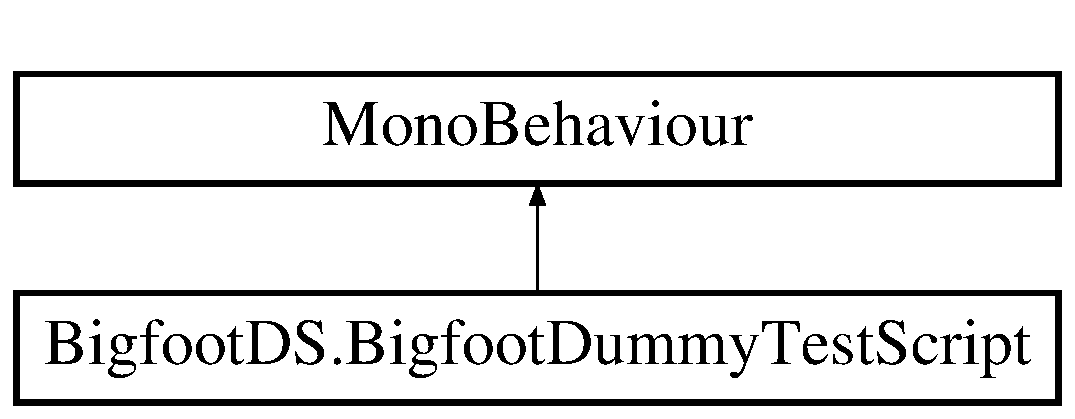
\includegraphics[height=2.000000cm]{class_bigfoot_d_s_1_1_bigfoot_dummy_test_script}
\end{center}
\end{figure}
\subsection*{Public Member Functions}
\begin{DoxyCompactItemize}
\item 
\mbox{\Hypertarget{class_bigfoot_d_s_1_1_bigfoot_dummy_test_script_a5e6dae54403c8d2f9f2828d6215d7b43}\label{class_bigfoot_d_s_1_1_bigfoot_dummy_test_script_a5e6dae54403c8d2f9f2828d6215d7b43}} 
void {\bfseries Dummy\+Test\+Roll\+D20} ()
\end{DoxyCompactItemize}
\subsection*{Public Attributes}
\begin{DoxyCompactItemize}
\item 
\mbox{\Hypertarget{class_bigfoot_d_s_1_1_bigfoot_dummy_test_script_adef9fade3a144affcd34352ebeb40920}\label{class_bigfoot_d_s_1_1_bigfoot_dummy_test_script_adef9fade3a144affcd34352ebeb40920}} 
int {\bfseries num\+Of\+Heads}
\item 
\mbox{\Hypertarget{class_bigfoot_d_s_1_1_bigfoot_dummy_test_script_a69c07d16341795395f15f8d368fbb805}\label{class_bigfoot_d_s_1_1_bigfoot_dummy_test_script_a69c07d16341795395f15f8d368fbb805}} 
int {\bfseries num\+Of\+Tails}
\item 
\mbox{\Hypertarget{class_bigfoot_d_s_1_1_bigfoot_dummy_test_script_a339ee60fc8f620a967362e4659453e78}\label{class_bigfoot_d_s_1_1_bigfoot_dummy_test_script_a339ee60fc8f620a967362e4659453e78}} 
List$<$ string $>$ {\bfseries coin\+Flip\+Results} = new List$<$string$>$()
\end{DoxyCompactItemize}


\subsection{Detailed Description}
Use this script to sandbox \& test other scripts, functions and features. 



The documentation for this class was generated from the following file\+:\begin{DoxyCompactItemize}
\item 
Assets/\+Bigfoot\+D\+S/\+\_\+\+Common/\+Scripts/Bigfoot\+Dummy\+Test\+Script.\+cs\end{DoxyCompactItemize}

\hypertarget{class_bigfoot_d_s_1_1_bigfoot_event_invoker}{}\section{Bigfoot\+D\+S.\+Bigfoot\+Event\+Invoker Class Reference}
\label{class_bigfoot_d_s_1_1_bigfoot_event_invoker}\index{Bigfoot\+D\+S.\+Bigfoot\+Event\+Invoker@{Bigfoot\+D\+S.\+Bigfoot\+Event\+Invoker}}
Inheritance diagram for Bigfoot\+D\+S.\+Bigfoot\+Event\+Invoker\+:\begin{figure}[H]
\begin{center}
\leavevmode
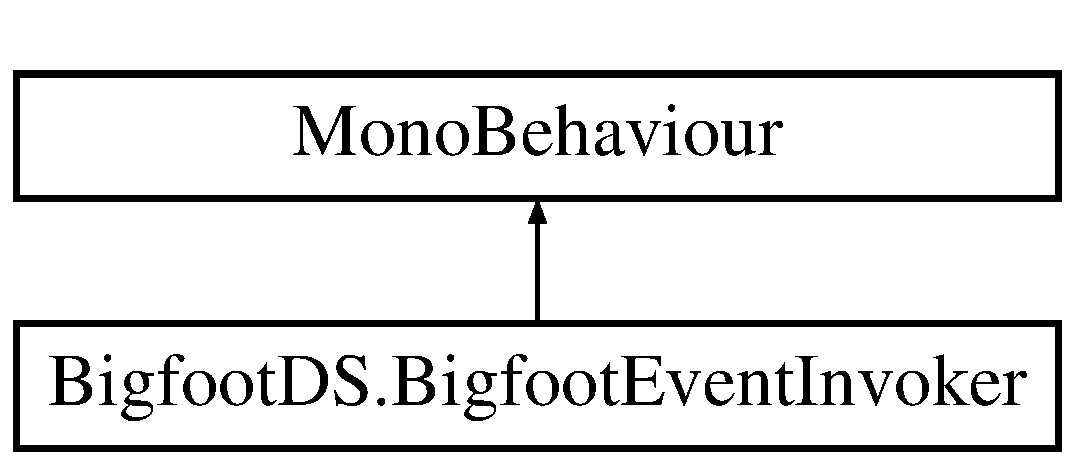
\includegraphics[height=2.000000cm]{class_bigfoot_d_s_1_1_bigfoot_event_invoker}
\end{center}
\end{figure}
\subsection*{Classes}
\begin{DoxyCompactItemize}
\item 
class \mbox{\hyperlink{class_bigfoot_d_s_1_1_bigfoot_event_invoker_1_1_specified_event}{Specified\+Event}}
\end{DoxyCompactItemize}
\subsection*{Public Member Functions}
\begin{DoxyCompactItemize}
\item 
\mbox{\Hypertarget{class_bigfoot_d_s_1_1_bigfoot_event_invoker_afd2da43c09f856aeae9c259dfec22c81}\label{class_bigfoot_d_s_1_1_bigfoot_event_invoker_afd2da43c09f856aeae9c259dfec22c81}} 
void {\bfseries Start\+Event\+Action} ()
\end{DoxyCompactItemize}
\subsection*{Public Attributes}
\begin{DoxyCompactItemize}
\item 
\mbox{\Hypertarget{class_bigfoot_d_s_1_1_bigfoot_event_invoker_adaaf1c060ccd20350f5d50955038c249}\label{class_bigfoot_d_s_1_1_bigfoot_event_invoker_adaaf1c060ccd20350f5d50955038c249}} 
\mbox{\hyperlink{class_bigfoot_d_s_1_1_bigfoot_event_invoker_1_1_specified_event}{Specified\+Event}} {\bfseries event\+Action} = new \mbox{\hyperlink{class_bigfoot_d_s_1_1_bigfoot_event_invoker_1_1_specified_event}{Specified\+Event}}()
\end{DoxyCompactItemize}


The documentation for this class was generated from the following file\+:\begin{DoxyCompactItemize}
\item 
Assets/\+Bigfoot\+D\+S/\+\_\+\+Common/\+Scripts/Bigfoot\+Event\+Invoker.\+cs\end{DoxyCompactItemize}

\hypertarget{class_bigfoot_d_s_1_1_bigfoot_general_location_finder}{}\section{Bigfoot\+D\+S.\+Bigfoot\+General\+Location\+Finder Class Reference}
\label{class_bigfoot_d_s_1_1_bigfoot_general_location_finder}\index{Bigfoot\+D\+S.\+Bigfoot\+General\+Location\+Finder@{Bigfoot\+D\+S.\+Bigfoot\+General\+Location\+Finder}}
Inheritance diagram for Bigfoot\+D\+S.\+Bigfoot\+General\+Location\+Finder\+:\begin{figure}[H]
\begin{center}
\leavevmode
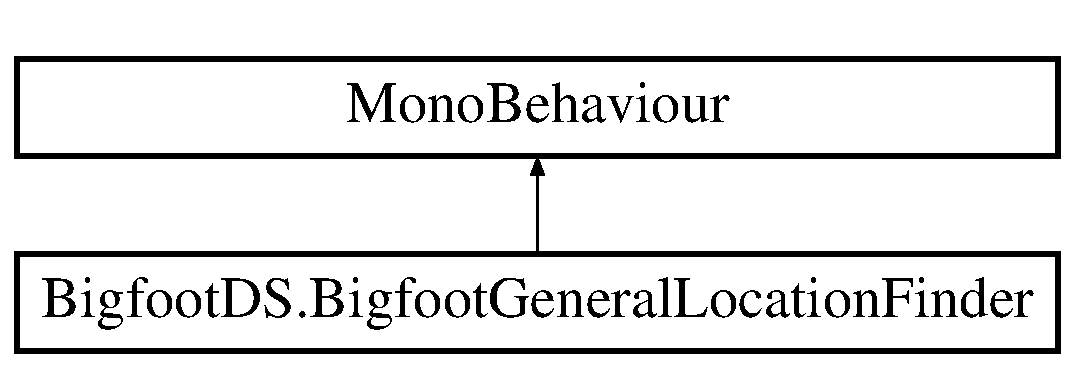
\includegraphics[height=2.000000cm]{class_bigfoot_d_s_1_1_bigfoot_general_location_finder}
\end{center}
\end{figure}
\subsection*{Public Member Functions}
\begin{DoxyCompactItemize}
\item 
void \mbox{\hyperlink{class_bigfoot_d_s_1_1_bigfoot_general_location_finder_a5e9cee69dcb8b0537be70f6e7ef8dba2}{Start\+R\+G\+Retrieval}} ()
\begin{DoxyCompactList}\small\item\em Alternative way to trigger the reverse-\/geocoding data-\/fetching coroutine -- incredibly important for UI \& button-\/based access. \end{DoxyCompactList}\item 
I\+Enumerator \mbox{\hyperlink{class_bigfoot_d_s_1_1_bigfoot_general_location_finder_a6fbed1e746517af8589df774e582771e}{Get\+Raw\+R\+G\+Data}} ()
\begin{DoxyCompactList}\small\item\em Retrieves the raw reverse-\/geocoding data about the player, based on their IP address. Requires internet access. \end{DoxyCompactList}\item 
void \mbox{\hyperlink{class_bigfoot_d_s_1_1_bigfoot_general_location_finder_a9740c9ca17041986a3c02e4597105b04}{Process\+R\+G\+Data}} ()
\begin{DoxyCompactList}\small\item\em Processes the data retrieved by the reverse-\/geocoding query and stores it as variables. Does not persist between sessions, so the query \& processing must be run at least once per session. \end{DoxyCompactList}\end{DoxyCompactItemize}
\subsection*{Public Attributes}
\begin{DoxyCompactItemize}
\item 
string \mbox{\hyperlink{class_bigfoot_d_s_1_1_bigfoot_general_location_finder_a76a67a66c34a490534022973b6ef8622}{raw\+R\+G\+Output}} = \char`\"{}\char`\"{}
\begin{DoxyCompactList}\small\item\em The raw data retrieved by the reverse-\/geocoding query. \end{DoxyCompactList}\item 
bool \mbox{\hyperlink{class_bigfoot_d_s_1_1_bigfoot_general_location_finder_a47dbb50a676cb53063ab0f648c93fc76}{successful\+RG}} = false
\begin{DoxyCompactList}\small\item\em True/false flag for the status of the reverse-\/geocoding query. \end{DoxyCompactList}\item 
string \mbox{\hyperlink{class_bigfoot_d_s_1_1_bigfoot_general_location_finder_a931f428edd0031ddf186903f148dd0a6}{user\+Country}}
\begin{DoxyCompactList}\small\item\em The user\textquotesingle{}s country based on their internet connection location. May be fooled by V\+PN setups. \end{DoxyCompactList}\item 
string \mbox{\hyperlink{class_bigfoot_d_s_1_1_bigfoot_general_location_finder_afe145b5b61a9f2a05493961ad7841e75}{user\+Country\+Code}}
\begin{DoxyCompactList}\small\item\em The user\textquotesingle{}s country code as per I\+SO 3166. \end{DoxyCompactList}\item 
string \mbox{\hyperlink{class_bigfoot_d_s_1_1_bigfoot_general_location_finder_a88c8886f1d052a9639468b53cba80eb1}{user\+Region\+Code}}
\begin{DoxyCompactList}\small\item\em The code for the user\textquotesingle{}s region or state. \end{DoxyCompactList}\item 
string \mbox{\hyperlink{class_bigfoot_d_s_1_1_bigfoot_general_location_finder_a0f4adca126c63bc34800d2d8a511ba87}{user\+Region\+Name}}
\begin{DoxyCompactList}\small\item\em The name of the user\textquotesingle{}s region or state. \end{DoxyCompactList}\item 
string \mbox{\hyperlink{class_bigfoot_d_s_1_1_bigfoot_general_location_finder_a05f1fa53a9892d4de8103fbe16858db2}{user\+City}}
\begin{DoxyCompactList}\small\item\em The name of the user\textquotesingle{}s city or town. \end{DoxyCompactList}\item 
string \mbox{\hyperlink{class_bigfoot_d_s_1_1_bigfoot_general_location_finder_a4db74322da4080833664faf84768f92c}{user\+Zip\+Code}}
\begin{DoxyCompactList}\small\item\em The Z\+IP or postal code of the user\textquotesingle{}s town or city. \end{DoxyCompactList}\item 
string \mbox{\hyperlink{class_bigfoot_d_s_1_1_bigfoot_general_location_finder_a821155456db788ade1ad0c53b30a4e82}{user\+Latitude}}
\begin{DoxyCompactList}\small\item\em The user\textquotesingle{}s latitude values. Due to the nature of I\+P-\/based requests, this will be very poor compared to a G\+PS coordinate. \end{DoxyCompactList}\item 
string \mbox{\hyperlink{class_bigfoot_d_s_1_1_bigfoot_general_location_finder_a6c99e8e8c60a7f003dfcf0474c77ef41}{user\+Longitude}}
\begin{DoxyCompactList}\small\item\em The user\textquotesingle{}s longitude values. Due to the nature of I\+P-\/based requests, this will be very poor compared to a G\+PS coordinate. \end{DoxyCompactList}\item 
string \mbox{\hyperlink{class_bigfoot_d_s_1_1_bigfoot_general_location_finder_ab443ecc804537beca860e12c3ff6c5cd}{user\+Time\+Zone}}
\begin{DoxyCompactList}\small\item\em The timezone for the user based on their location (not the built-\/in device timezone). \end{DoxyCompactList}\item 
string \mbox{\hyperlink{class_bigfoot_d_s_1_1_bigfoot_general_location_finder_a1269e7e1706072b54b099191ee3c4f59}{user\+I\+S\+P\+Name}}
\begin{DoxyCompactList}\small\item\em The user\textquotesingle{}s internet provider. \end{DoxyCompactList}\item 
string \mbox{\hyperlink{class_bigfoot_d_s_1_1_bigfoot_general_location_finder_a410dad417fd2d229d2caf1474107364c}{user\+Organization\+Name}}
\begin{DoxyCompactList}\small\item\em The user\textquotesingle{}s internet organization (usually the same as the I\+SP). \end{DoxyCompactList}\item 
string \mbox{\hyperlink{class_bigfoot_d_s_1_1_bigfoot_general_location_finder_a973995199b617a6d6b40c4c7a331f5de}{user\+Autonomous\+System\+Code}}
\begin{DoxyCompactList}\small\item\em The user\textquotesingle{}s internet autonomous system number and name. \end{DoxyCompactList}\item 
string \mbox{\hyperlink{class_bigfoot_d_s_1_1_bigfoot_general_location_finder_ab1b2e2503b22529b0936c9c9ba8b88e0}{user\+I\+P\+Address}}
\begin{DoxyCompactList}\small\item\em The IP address used for the reverse-\/geocoding query. \end{DoxyCompactList}\end{DoxyCompactItemize}


\subsection{Member Function Documentation}
\mbox{\Hypertarget{class_bigfoot_d_s_1_1_bigfoot_general_location_finder_a6fbed1e746517af8589df774e582771e}\label{class_bigfoot_d_s_1_1_bigfoot_general_location_finder_a6fbed1e746517af8589df774e582771e}} 
\index{Bigfoot\+D\+S\+::\+Bigfoot\+General\+Location\+Finder@{Bigfoot\+D\+S\+::\+Bigfoot\+General\+Location\+Finder}!Get\+Raw\+R\+G\+Data@{Get\+Raw\+R\+G\+Data}}
\index{Get\+Raw\+R\+G\+Data@{Get\+Raw\+R\+G\+Data}!Bigfoot\+D\+S\+::\+Bigfoot\+General\+Location\+Finder@{Bigfoot\+D\+S\+::\+Bigfoot\+General\+Location\+Finder}}
\subsubsection{\texorpdfstring{Get\+Raw\+R\+G\+Data()}{GetRawRGData()}}
{\footnotesize\ttfamily I\+Enumerator Bigfoot\+D\+S.\+Bigfoot\+General\+Location\+Finder.\+Get\+Raw\+R\+G\+Data (\begin{DoxyParamCaption}{ }\end{DoxyParamCaption})}



Retrieves the raw reverse-\/geocoding data about the player, based on their IP address. Requires internet access. 

\mbox{\Hypertarget{class_bigfoot_d_s_1_1_bigfoot_general_location_finder_a9740c9ca17041986a3c02e4597105b04}\label{class_bigfoot_d_s_1_1_bigfoot_general_location_finder_a9740c9ca17041986a3c02e4597105b04}} 
\index{Bigfoot\+D\+S\+::\+Bigfoot\+General\+Location\+Finder@{Bigfoot\+D\+S\+::\+Bigfoot\+General\+Location\+Finder}!Process\+R\+G\+Data@{Process\+R\+G\+Data}}
\index{Process\+R\+G\+Data@{Process\+R\+G\+Data}!Bigfoot\+D\+S\+::\+Bigfoot\+General\+Location\+Finder@{Bigfoot\+D\+S\+::\+Bigfoot\+General\+Location\+Finder}}
\subsubsection{\texorpdfstring{Process\+R\+G\+Data()}{ProcessRGData()}}
{\footnotesize\ttfamily void Bigfoot\+D\+S.\+Bigfoot\+General\+Location\+Finder.\+Process\+R\+G\+Data (\begin{DoxyParamCaption}{ }\end{DoxyParamCaption})}



Processes the data retrieved by the reverse-\/geocoding query and stores it as variables. Does not persist between sessions, so the query \& processing must be run at least once per session. 

Automatically sanitizes outputs (eg. removing quotation marks) so any \& all information can be instantly used by other scripts \& functions. \mbox{\Hypertarget{class_bigfoot_d_s_1_1_bigfoot_general_location_finder_a5e9cee69dcb8b0537be70f6e7ef8dba2}\label{class_bigfoot_d_s_1_1_bigfoot_general_location_finder_a5e9cee69dcb8b0537be70f6e7ef8dba2}} 
\index{Bigfoot\+D\+S\+::\+Bigfoot\+General\+Location\+Finder@{Bigfoot\+D\+S\+::\+Bigfoot\+General\+Location\+Finder}!Start\+R\+G\+Retrieval@{Start\+R\+G\+Retrieval}}
\index{Start\+R\+G\+Retrieval@{Start\+R\+G\+Retrieval}!Bigfoot\+D\+S\+::\+Bigfoot\+General\+Location\+Finder@{Bigfoot\+D\+S\+::\+Bigfoot\+General\+Location\+Finder}}
\subsubsection{\texorpdfstring{Start\+R\+G\+Retrieval()}{StartRGRetrieval()}}
{\footnotesize\ttfamily void Bigfoot\+D\+S.\+Bigfoot\+General\+Location\+Finder.\+Start\+R\+G\+Retrieval (\begin{DoxyParamCaption}{ }\end{DoxyParamCaption})}



Alternative way to trigger the reverse-\/geocoding data-\/fetching coroutine -- incredibly important for UI \& button-\/based access. 



\subsection{Member Data Documentation}
\mbox{\Hypertarget{class_bigfoot_d_s_1_1_bigfoot_general_location_finder_a76a67a66c34a490534022973b6ef8622}\label{class_bigfoot_d_s_1_1_bigfoot_general_location_finder_a76a67a66c34a490534022973b6ef8622}} 
\index{Bigfoot\+D\+S\+::\+Bigfoot\+General\+Location\+Finder@{Bigfoot\+D\+S\+::\+Bigfoot\+General\+Location\+Finder}!raw\+R\+G\+Output@{raw\+R\+G\+Output}}
\index{raw\+R\+G\+Output@{raw\+R\+G\+Output}!Bigfoot\+D\+S\+::\+Bigfoot\+General\+Location\+Finder@{Bigfoot\+D\+S\+::\+Bigfoot\+General\+Location\+Finder}}
\subsubsection{\texorpdfstring{raw\+R\+G\+Output}{rawRGOutput}}
{\footnotesize\ttfamily string Bigfoot\+D\+S.\+Bigfoot\+General\+Location\+Finder.\+raw\+R\+G\+Output = \char`\"{}\char`\"{}}



The raw data retrieved by the reverse-\/geocoding query. 

\mbox{\Hypertarget{class_bigfoot_d_s_1_1_bigfoot_general_location_finder_a47dbb50a676cb53063ab0f648c93fc76}\label{class_bigfoot_d_s_1_1_bigfoot_general_location_finder_a47dbb50a676cb53063ab0f648c93fc76}} 
\index{Bigfoot\+D\+S\+::\+Bigfoot\+General\+Location\+Finder@{Bigfoot\+D\+S\+::\+Bigfoot\+General\+Location\+Finder}!successful\+RG@{successful\+RG}}
\index{successful\+RG@{successful\+RG}!Bigfoot\+D\+S\+::\+Bigfoot\+General\+Location\+Finder@{Bigfoot\+D\+S\+::\+Bigfoot\+General\+Location\+Finder}}
\subsubsection{\texorpdfstring{successful\+RG}{successfulRG}}
{\footnotesize\ttfamily bool Bigfoot\+D\+S.\+Bigfoot\+General\+Location\+Finder.\+successful\+RG = false}



True/false flag for the status of the reverse-\/geocoding query. 

\mbox{\Hypertarget{class_bigfoot_d_s_1_1_bigfoot_general_location_finder_a973995199b617a6d6b40c4c7a331f5de}\label{class_bigfoot_d_s_1_1_bigfoot_general_location_finder_a973995199b617a6d6b40c4c7a331f5de}} 
\index{Bigfoot\+D\+S\+::\+Bigfoot\+General\+Location\+Finder@{Bigfoot\+D\+S\+::\+Bigfoot\+General\+Location\+Finder}!user\+Autonomous\+System\+Code@{user\+Autonomous\+System\+Code}}
\index{user\+Autonomous\+System\+Code@{user\+Autonomous\+System\+Code}!Bigfoot\+D\+S\+::\+Bigfoot\+General\+Location\+Finder@{Bigfoot\+D\+S\+::\+Bigfoot\+General\+Location\+Finder}}
\subsubsection{\texorpdfstring{user\+Autonomous\+System\+Code}{userAutonomousSystemCode}}
{\footnotesize\ttfamily string Bigfoot\+D\+S.\+Bigfoot\+General\+Location\+Finder.\+user\+Autonomous\+System\+Code}



The user\textquotesingle{}s internet autonomous system number and name. 

\mbox{\Hypertarget{class_bigfoot_d_s_1_1_bigfoot_general_location_finder_a05f1fa53a9892d4de8103fbe16858db2}\label{class_bigfoot_d_s_1_1_bigfoot_general_location_finder_a05f1fa53a9892d4de8103fbe16858db2}} 
\index{Bigfoot\+D\+S\+::\+Bigfoot\+General\+Location\+Finder@{Bigfoot\+D\+S\+::\+Bigfoot\+General\+Location\+Finder}!user\+City@{user\+City}}
\index{user\+City@{user\+City}!Bigfoot\+D\+S\+::\+Bigfoot\+General\+Location\+Finder@{Bigfoot\+D\+S\+::\+Bigfoot\+General\+Location\+Finder}}
\subsubsection{\texorpdfstring{user\+City}{userCity}}
{\footnotesize\ttfamily string Bigfoot\+D\+S.\+Bigfoot\+General\+Location\+Finder.\+user\+City}



The name of the user\textquotesingle{}s city or town. 

\mbox{\Hypertarget{class_bigfoot_d_s_1_1_bigfoot_general_location_finder_a931f428edd0031ddf186903f148dd0a6}\label{class_bigfoot_d_s_1_1_bigfoot_general_location_finder_a931f428edd0031ddf186903f148dd0a6}} 
\index{Bigfoot\+D\+S\+::\+Bigfoot\+General\+Location\+Finder@{Bigfoot\+D\+S\+::\+Bigfoot\+General\+Location\+Finder}!user\+Country@{user\+Country}}
\index{user\+Country@{user\+Country}!Bigfoot\+D\+S\+::\+Bigfoot\+General\+Location\+Finder@{Bigfoot\+D\+S\+::\+Bigfoot\+General\+Location\+Finder}}
\subsubsection{\texorpdfstring{user\+Country}{userCountry}}
{\footnotesize\ttfamily string Bigfoot\+D\+S.\+Bigfoot\+General\+Location\+Finder.\+user\+Country}



The user\textquotesingle{}s country based on their internet connection location. May be fooled by V\+PN setups. 

\mbox{\Hypertarget{class_bigfoot_d_s_1_1_bigfoot_general_location_finder_afe145b5b61a9f2a05493961ad7841e75}\label{class_bigfoot_d_s_1_1_bigfoot_general_location_finder_afe145b5b61a9f2a05493961ad7841e75}} 
\index{Bigfoot\+D\+S\+::\+Bigfoot\+General\+Location\+Finder@{Bigfoot\+D\+S\+::\+Bigfoot\+General\+Location\+Finder}!user\+Country\+Code@{user\+Country\+Code}}
\index{user\+Country\+Code@{user\+Country\+Code}!Bigfoot\+D\+S\+::\+Bigfoot\+General\+Location\+Finder@{Bigfoot\+D\+S\+::\+Bigfoot\+General\+Location\+Finder}}
\subsubsection{\texorpdfstring{user\+Country\+Code}{userCountryCode}}
{\footnotesize\ttfamily string Bigfoot\+D\+S.\+Bigfoot\+General\+Location\+Finder.\+user\+Country\+Code}



The user\textquotesingle{}s country code as per I\+SO 3166. 

\mbox{\Hypertarget{class_bigfoot_d_s_1_1_bigfoot_general_location_finder_ab1b2e2503b22529b0936c9c9ba8b88e0}\label{class_bigfoot_d_s_1_1_bigfoot_general_location_finder_ab1b2e2503b22529b0936c9c9ba8b88e0}} 
\index{Bigfoot\+D\+S\+::\+Bigfoot\+General\+Location\+Finder@{Bigfoot\+D\+S\+::\+Bigfoot\+General\+Location\+Finder}!user\+I\+P\+Address@{user\+I\+P\+Address}}
\index{user\+I\+P\+Address@{user\+I\+P\+Address}!Bigfoot\+D\+S\+::\+Bigfoot\+General\+Location\+Finder@{Bigfoot\+D\+S\+::\+Bigfoot\+General\+Location\+Finder}}
\subsubsection{\texorpdfstring{user\+I\+P\+Address}{userIPAddress}}
{\footnotesize\ttfamily string Bigfoot\+D\+S.\+Bigfoot\+General\+Location\+Finder.\+user\+I\+P\+Address}



The IP address used for the reverse-\/geocoding query. 

\mbox{\Hypertarget{class_bigfoot_d_s_1_1_bigfoot_general_location_finder_a1269e7e1706072b54b099191ee3c4f59}\label{class_bigfoot_d_s_1_1_bigfoot_general_location_finder_a1269e7e1706072b54b099191ee3c4f59}} 
\index{Bigfoot\+D\+S\+::\+Bigfoot\+General\+Location\+Finder@{Bigfoot\+D\+S\+::\+Bigfoot\+General\+Location\+Finder}!user\+I\+S\+P\+Name@{user\+I\+S\+P\+Name}}
\index{user\+I\+S\+P\+Name@{user\+I\+S\+P\+Name}!Bigfoot\+D\+S\+::\+Bigfoot\+General\+Location\+Finder@{Bigfoot\+D\+S\+::\+Bigfoot\+General\+Location\+Finder}}
\subsubsection{\texorpdfstring{user\+I\+S\+P\+Name}{userISPName}}
{\footnotesize\ttfamily string Bigfoot\+D\+S.\+Bigfoot\+General\+Location\+Finder.\+user\+I\+S\+P\+Name}



The user\textquotesingle{}s internet provider. 

\mbox{\Hypertarget{class_bigfoot_d_s_1_1_bigfoot_general_location_finder_a821155456db788ade1ad0c53b30a4e82}\label{class_bigfoot_d_s_1_1_bigfoot_general_location_finder_a821155456db788ade1ad0c53b30a4e82}} 
\index{Bigfoot\+D\+S\+::\+Bigfoot\+General\+Location\+Finder@{Bigfoot\+D\+S\+::\+Bigfoot\+General\+Location\+Finder}!user\+Latitude@{user\+Latitude}}
\index{user\+Latitude@{user\+Latitude}!Bigfoot\+D\+S\+::\+Bigfoot\+General\+Location\+Finder@{Bigfoot\+D\+S\+::\+Bigfoot\+General\+Location\+Finder}}
\subsubsection{\texorpdfstring{user\+Latitude}{userLatitude}}
{\footnotesize\ttfamily string Bigfoot\+D\+S.\+Bigfoot\+General\+Location\+Finder.\+user\+Latitude}



The user\textquotesingle{}s latitude values. Due to the nature of I\+P-\/based requests, this will be very poor compared to a G\+PS coordinate. 

\mbox{\Hypertarget{class_bigfoot_d_s_1_1_bigfoot_general_location_finder_a6c99e8e8c60a7f003dfcf0474c77ef41}\label{class_bigfoot_d_s_1_1_bigfoot_general_location_finder_a6c99e8e8c60a7f003dfcf0474c77ef41}} 
\index{Bigfoot\+D\+S\+::\+Bigfoot\+General\+Location\+Finder@{Bigfoot\+D\+S\+::\+Bigfoot\+General\+Location\+Finder}!user\+Longitude@{user\+Longitude}}
\index{user\+Longitude@{user\+Longitude}!Bigfoot\+D\+S\+::\+Bigfoot\+General\+Location\+Finder@{Bigfoot\+D\+S\+::\+Bigfoot\+General\+Location\+Finder}}
\subsubsection{\texorpdfstring{user\+Longitude}{userLongitude}}
{\footnotesize\ttfamily string Bigfoot\+D\+S.\+Bigfoot\+General\+Location\+Finder.\+user\+Longitude}



The user\textquotesingle{}s longitude values. Due to the nature of I\+P-\/based requests, this will be very poor compared to a G\+PS coordinate. 

\mbox{\Hypertarget{class_bigfoot_d_s_1_1_bigfoot_general_location_finder_a410dad417fd2d229d2caf1474107364c}\label{class_bigfoot_d_s_1_1_bigfoot_general_location_finder_a410dad417fd2d229d2caf1474107364c}} 
\index{Bigfoot\+D\+S\+::\+Bigfoot\+General\+Location\+Finder@{Bigfoot\+D\+S\+::\+Bigfoot\+General\+Location\+Finder}!user\+Organization\+Name@{user\+Organization\+Name}}
\index{user\+Organization\+Name@{user\+Organization\+Name}!Bigfoot\+D\+S\+::\+Bigfoot\+General\+Location\+Finder@{Bigfoot\+D\+S\+::\+Bigfoot\+General\+Location\+Finder}}
\subsubsection{\texorpdfstring{user\+Organization\+Name}{userOrganizationName}}
{\footnotesize\ttfamily string Bigfoot\+D\+S.\+Bigfoot\+General\+Location\+Finder.\+user\+Organization\+Name}



The user\textquotesingle{}s internet organization (usually the same as the I\+SP). 

\mbox{\Hypertarget{class_bigfoot_d_s_1_1_bigfoot_general_location_finder_a88c8886f1d052a9639468b53cba80eb1}\label{class_bigfoot_d_s_1_1_bigfoot_general_location_finder_a88c8886f1d052a9639468b53cba80eb1}} 
\index{Bigfoot\+D\+S\+::\+Bigfoot\+General\+Location\+Finder@{Bigfoot\+D\+S\+::\+Bigfoot\+General\+Location\+Finder}!user\+Region\+Code@{user\+Region\+Code}}
\index{user\+Region\+Code@{user\+Region\+Code}!Bigfoot\+D\+S\+::\+Bigfoot\+General\+Location\+Finder@{Bigfoot\+D\+S\+::\+Bigfoot\+General\+Location\+Finder}}
\subsubsection{\texorpdfstring{user\+Region\+Code}{userRegionCode}}
{\footnotesize\ttfamily string Bigfoot\+D\+S.\+Bigfoot\+General\+Location\+Finder.\+user\+Region\+Code}



The code for the user\textquotesingle{}s region or state. 

\mbox{\Hypertarget{class_bigfoot_d_s_1_1_bigfoot_general_location_finder_a0f4adca126c63bc34800d2d8a511ba87}\label{class_bigfoot_d_s_1_1_bigfoot_general_location_finder_a0f4adca126c63bc34800d2d8a511ba87}} 
\index{Bigfoot\+D\+S\+::\+Bigfoot\+General\+Location\+Finder@{Bigfoot\+D\+S\+::\+Bigfoot\+General\+Location\+Finder}!user\+Region\+Name@{user\+Region\+Name}}
\index{user\+Region\+Name@{user\+Region\+Name}!Bigfoot\+D\+S\+::\+Bigfoot\+General\+Location\+Finder@{Bigfoot\+D\+S\+::\+Bigfoot\+General\+Location\+Finder}}
\subsubsection{\texorpdfstring{user\+Region\+Name}{userRegionName}}
{\footnotesize\ttfamily string Bigfoot\+D\+S.\+Bigfoot\+General\+Location\+Finder.\+user\+Region\+Name}



The name of the user\textquotesingle{}s region or state. 

\mbox{\Hypertarget{class_bigfoot_d_s_1_1_bigfoot_general_location_finder_ab443ecc804537beca860e12c3ff6c5cd}\label{class_bigfoot_d_s_1_1_bigfoot_general_location_finder_ab443ecc804537beca860e12c3ff6c5cd}} 
\index{Bigfoot\+D\+S\+::\+Bigfoot\+General\+Location\+Finder@{Bigfoot\+D\+S\+::\+Bigfoot\+General\+Location\+Finder}!user\+Time\+Zone@{user\+Time\+Zone}}
\index{user\+Time\+Zone@{user\+Time\+Zone}!Bigfoot\+D\+S\+::\+Bigfoot\+General\+Location\+Finder@{Bigfoot\+D\+S\+::\+Bigfoot\+General\+Location\+Finder}}
\subsubsection{\texorpdfstring{user\+Time\+Zone}{userTimeZone}}
{\footnotesize\ttfamily string Bigfoot\+D\+S.\+Bigfoot\+General\+Location\+Finder.\+user\+Time\+Zone}



The timezone for the user based on their location (not the built-\/in device timezone). 

\mbox{\Hypertarget{class_bigfoot_d_s_1_1_bigfoot_general_location_finder_a4db74322da4080833664faf84768f92c}\label{class_bigfoot_d_s_1_1_bigfoot_general_location_finder_a4db74322da4080833664faf84768f92c}} 
\index{Bigfoot\+D\+S\+::\+Bigfoot\+General\+Location\+Finder@{Bigfoot\+D\+S\+::\+Bigfoot\+General\+Location\+Finder}!user\+Zip\+Code@{user\+Zip\+Code}}
\index{user\+Zip\+Code@{user\+Zip\+Code}!Bigfoot\+D\+S\+::\+Bigfoot\+General\+Location\+Finder@{Bigfoot\+D\+S\+::\+Bigfoot\+General\+Location\+Finder}}
\subsubsection{\texorpdfstring{user\+Zip\+Code}{userZipCode}}
{\footnotesize\ttfamily string Bigfoot\+D\+S.\+Bigfoot\+General\+Location\+Finder.\+user\+Zip\+Code}



The Z\+IP or postal code of the user\textquotesingle{}s town or city. 



The documentation for this class was generated from the following file\+:\begin{DoxyCompactItemize}
\item 
Assets/\+Bigfoot\+D\+S/\+\_\+\+Common/\+Scripts/Bigfoot\+General\+Location\+Finder.\+cs\end{DoxyCompactItemize}

\hypertarget{class_bigfoot_d_s_1_1_bigfoot_normals_inverter}{}\section{Bigfoot\+D\+S.\+Bigfoot\+Normals\+Inverter Class Reference}
\label{class_bigfoot_d_s_1_1_bigfoot_normals_inverter}\index{Bigfoot\+D\+S.\+Bigfoot\+Normals\+Inverter@{Bigfoot\+D\+S.\+Bigfoot\+Normals\+Inverter}}
Inheritance diagram for Bigfoot\+D\+S.\+Bigfoot\+Normals\+Inverter\+:\begin{figure}[H]
\begin{center}
\leavevmode
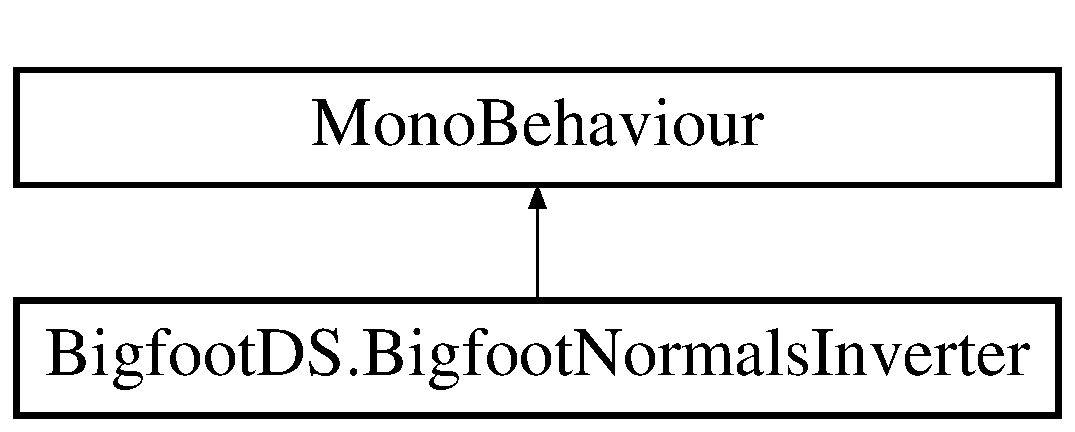
\includegraphics[height=2.000000cm]{class_bigfoot_d_s_1_1_bigfoot_normals_inverter}
\end{center}
\end{figure}
\subsection*{Public Member Functions}
\begin{DoxyCompactItemize}
\item 
void \mbox{\hyperlink{class_bigfoot_d_s_1_1_bigfoot_normals_inverter_aa1e69f42fcba0e36398db1e8fd7d217f}{Invert\+Mesh\+Normals}} ()
\begin{DoxyCompactList}\small\item\em Inverts the normals of a mesh as specified by the \mbox{\hyperlink{class_bigfoot_d_s_1_1_bigfoot_normals_inverter}{Bigfoot\+Normals\+Inverter}} component. \end{DoxyCompactList}\end{DoxyCompactItemize}
\subsection*{Public Attributes}
\begin{DoxyCompactItemize}
\item 
Mesh\+Filter \mbox{\hyperlink{class_bigfoot_d_s_1_1_bigfoot_normals_inverter_ae9f17ad0ec0cc214b044d8ee8f5c6ba7}{mesh\+To\+Invert}}
\begin{DoxyCompactList}\small\item\em The specified mesh that will have its normals inverted. The script will automatically fetch this component on the same object if this field is left blank. \end{DoxyCompactList}\item 
bool \mbox{\hyperlink{class_bigfoot_d_s_1_1_bigfoot_normals_inverter_aafe7464bb4afaa60822e2463d541bf77}{auto\+Inverter}} = true
\begin{DoxyCompactList}\small\item\em If enabled, this will invert the normals of the desired mesh as soon as physically possible. \end{DoxyCompactList}\end{DoxyCompactItemize}


\subsection{Member Function Documentation}
\mbox{\Hypertarget{class_bigfoot_d_s_1_1_bigfoot_normals_inverter_aa1e69f42fcba0e36398db1e8fd7d217f}\label{class_bigfoot_d_s_1_1_bigfoot_normals_inverter_aa1e69f42fcba0e36398db1e8fd7d217f}} 
\index{Bigfoot\+D\+S\+::\+Bigfoot\+Normals\+Inverter@{Bigfoot\+D\+S\+::\+Bigfoot\+Normals\+Inverter}!Invert\+Mesh\+Normals@{Invert\+Mesh\+Normals}}
\index{Invert\+Mesh\+Normals@{Invert\+Mesh\+Normals}!Bigfoot\+D\+S\+::\+Bigfoot\+Normals\+Inverter@{Bigfoot\+D\+S\+::\+Bigfoot\+Normals\+Inverter}}
\subsubsection{\texorpdfstring{Invert\+Mesh\+Normals()}{InvertMeshNormals()}}
{\footnotesize\ttfamily void Bigfoot\+D\+S.\+Bigfoot\+Normals\+Inverter.\+Invert\+Mesh\+Normals (\begin{DoxyParamCaption}{ }\end{DoxyParamCaption})}



Inverts the normals of a mesh as specified by the \mbox{\hyperlink{class_bigfoot_d_s_1_1_bigfoot_normals_inverter}{Bigfoot\+Normals\+Inverter}} component. 



\subsection{Member Data Documentation}
\mbox{\Hypertarget{class_bigfoot_d_s_1_1_bigfoot_normals_inverter_aafe7464bb4afaa60822e2463d541bf77}\label{class_bigfoot_d_s_1_1_bigfoot_normals_inverter_aafe7464bb4afaa60822e2463d541bf77}} 
\index{Bigfoot\+D\+S\+::\+Bigfoot\+Normals\+Inverter@{Bigfoot\+D\+S\+::\+Bigfoot\+Normals\+Inverter}!auto\+Inverter@{auto\+Inverter}}
\index{auto\+Inverter@{auto\+Inverter}!Bigfoot\+D\+S\+::\+Bigfoot\+Normals\+Inverter@{Bigfoot\+D\+S\+::\+Bigfoot\+Normals\+Inverter}}
\subsubsection{\texorpdfstring{auto\+Inverter}{autoInverter}}
{\footnotesize\ttfamily bool Bigfoot\+D\+S.\+Bigfoot\+Normals\+Inverter.\+auto\+Inverter = true}



If enabled, this will invert the normals of the desired mesh as soon as physically possible. 

\mbox{\Hypertarget{class_bigfoot_d_s_1_1_bigfoot_normals_inverter_ae9f17ad0ec0cc214b044d8ee8f5c6ba7}\label{class_bigfoot_d_s_1_1_bigfoot_normals_inverter_ae9f17ad0ec0cc214b044d8ee8f5c6ba7}} 
\index{Bigfoot\+D\+S\+::\+Bigfoot\+Normals\+Inverter@{Bigfoot\+D\+S\+::\+Bigfoot\+Normals\+Inverter}!mesh\+To\+Invert@{mesh\+To\+Invert}}
\index{mesh\+To\+Invert@{mesh\+To\+Invert}!Bigfoot\+D\+S\+::\+Bigfoot\+Normals\+Inverter@{Bigfoot\+D\+S\+::\+Bigfoot\+Normals\+Inverter}}
\subsubsection{\texorpdfstring{mesh\+To\+Invert}{meshToInvert}}
{\footnotesize\ttfamily Mesh\+Filter Bigfoot\+D\+S.\+Bigfoot\+Normals\+Inverter.\+mesh\+To\+Invert}



The specified mesh that will have its normals inverted. The script will automatically fetch this component on the same object if this field is left blank. 



The documentation for this class was generated from the following file\+:\begin{DoxyCompactItemize}
\item 
Assets/\+Bigfoot\+D\+S/\+\_\+\+Common/\+Scripts/Bigfoot\+Normals\+Inverter.\+cs\end{DoxyCompactItemize}

\hypertarget{class_bigfoot_d_s_1_1_bigfoot_web_colours_default}{}\section{Bigfoot\+D\+S.\+Bigfoot\+Web\+Colours\+Default Class Reference}
\label{class_bigfoot_d_s_1_1_bigfoot_web_colours_default}\index{Bigfoot\+D\+S.\+Bigfoot\+Web\+Colours\+Default@{Bigfoot\+D\+S.\+Bigfoot\+Web\+Colours\+Default}}
Inheritance diagram for Bigfoot\+D\+S.\+Bigfoot\+Web\+Colours\+Default\+:\begin{figure}[H]
\begin{center}
\leavevmode
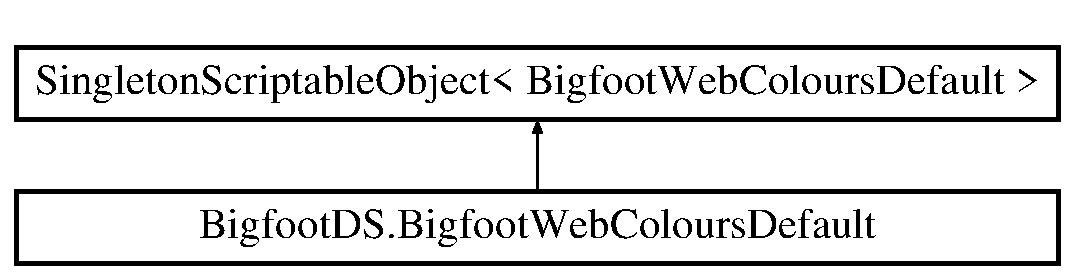
\includegraphics[height=2.000000cm]{class_bigfoot_d_s_1_1_bigfoot_web_colours_default}
\end{center}
\end{figure}
\subsection*{Public Attributes}
\begin{DoxyCompactItemize}
\item 
\mbox{\Hypertarget{class_bigfoot_d_s_1_1_bigfoot_web_colours_default_acb7f51ad30edde89fca17531172b3b47}\label{class_bigfoot_d_s_1_1_bigfoot_web_colours_default_acb7f51ad30edde89fca17531172b3b47}} 
Material {\bfseries Alice\+Blue}
\item 
\mbox{\Hypertarget{class_bigfoot_d_s_1_1_bigfoot_web_colours_default_a6c9b9a2255a6012b125ca165ffe75fab}\label{class_bigfoot_d_s_1_1_bigfoot_web_colours_default_a6c9b9a2255a6012b125ca165ffe75fab}} 
Material {\bfseries Antique\+White}
\item 
\mbox{\Hypertarget{class_bigfoot_d_s_1_1_bigfoot_web_colours_default_a3f993e527ef32089774b8d1309de223a}\label{class_bigfoot_d_s_1_1_bigfoot_web_colours_default_a3f993e527ef32089774b8d1309de223a}} 
Material {\bfseries Aqua}
\item 
\mbox{\Hypertarget{class_bigfoot_d_s_1_1_bigfoot_web_colours_default_a69a0c2d39934d9c8f6e0a6614cbf5212}\label{class_bigfoot_d_s_1_1_bigfoot_web_colours_default_a69a0c2d39934d9c8f6e0a6614cbf5212}} 
Material {\bfseries Aquamarine}
\item 
\mbox{\Hypertarget{class_bigfoot_d_s_1_1_bigfoot_web_colours_default_a0c6c1a12a127c8448136b5843d0a9403}\label{class_bigfoot_d_s_1_1_bigfoot_web_colours_default_a0c6c1a12a127c8448136b5843d0a9403}} 
Material {\bfseries Azure}
\item 
\mbox{\Hypertarget{class_bigfoot_d_s_1_1_bigfoot_web_colours_default_a423c7fbcf4879ee30cc48b4ad061dabd}\label{class_bigfoot_d_s_1_1_bigfoot_web_colours_default_a423c7fbcf4879ee30cc48b4ad061dabd}} 
Material {\bfseries Beige}
\item 
\mbox{\Hypertarget{class_bigfoot_d_s_1_1_bigfoot_web_colours_default_ad728ad408f35e3dd4b3b838962036200}\label{class_bigfoot_d_s_1_1_bigfoot_web_colours_default_ad728ad408f35e3dd4b3b838962036200}} 
Material {\bfseries Bisque}
\item 
\mbox{\Hypertarget{class_bigfoot_d_s_1_1_bigfoot_web_colours_default_ac4d816bf04e905da43a7a48bbddc7166}\label{class_bigfoot_d_s_1_1_bigfoot_web_colours_default_ac4d816bf04e905da43a7a48bbddc7166}} 
Material {\bfseries Black}
\item 
\mbox{\Hypertarget{class_bigfoot_d_s_1_1_bigfoot_web_colours_default_a55e352329131f61108f566f07690feed}\label{class_bigfoot_d_s_1_1_bigfoot_web_colours_default_a55e352329131f61108f566f07690feed}} 
Material {\bfseries Blanched\+Almond}
\item 
\mbox{\Hypertarget{class_bigfoot_d_s_1_1_bigfoot_web_colours_default_a4c520bed751a1f6a60a027d470ac9521}\label{class_bigfoot_d_s_1_1_bigfoot_web_colours_default_a4c520bed751a1f6a60a027d470ac9521}} 
Material {\bfseries Blue}
\item 
\mbox{\Hypertarget{class_bigfoot_d_s_1_1_bigfoot_web_colours_default_a39d76d1fc08df7451906d45d33e0ab03}\label{class_bigfoot_d_s_1_1_bigfoot_web_colours_default_a39d76d1fc08df7451906d45d33e0ab03}} 
Material {\bfseries Blue\+Violet}
\item 
\mbox{\Hypertarget{class_bigfoot_d_s_1_1_bigfoot_web_colours_default_a83ec50d9953fd0cfdca9df8d71d7cfd3}\label{class_bigfoot_d_s_1_1_bigfoot_web_colours_default_a83ec50d9953fd0cfdca9df8d71d7cfd3}} 
Material {\bfseries Brown}
\item 
\mbox{\Hypertarget{class_bigfoot_d_s_1_1_bigfoot_web_colours_default_abe2a61e718dd81649079cb7bfc407046}\label{class_bigfoot_d_s_1_1_bigfoot_web_colours_default_abe2a61e718dd81649079cb7bfc407046}} 
Material {\bfseries Burly\+Wood}
\item 
\mbox{\Hypertarget{class_bigfoot_d_s_1_1_bigfoot_web_colours_default_a96376a1f2399e687611d72a87d5ab207}\label{class_bigfoot_d_s_1_1_bigfoot_web_colours_default_a96376a1f2399e687611d72a87d5ab207}} 
Material {\bfseries Cadet\+Blue}
\item 
\mbox{\Hypertarget{class_bigfoot_d_s_1_1_bigfoot_web_colours_default_a772c342d23d780356320bcedc384ec61}\label{class_bigfoot_d_s_1_1_bigfoot_web_colours_default_a772c342d23d780356320bcedc384ec61}} 
Material {\bfseries Chartreuse}
\item 
\mbox{\Hypertarget{class_bigfoot_d_s_1_1_bigfoot_web_colours_default_a95fc0803048bc6c44fb501d8382647a4}\label{class_bigfoot_d_s_1_1_bigfoot_web_colours_default_a95fc0803048bc6c44fb501d8382647a4}} 
Material {\bfseries Chocolate}
\item 
\mbox{\Hypertarget{class_bigfoot_d_s_1_1_bigfoot_web_colours_default_a57872f38a0a0dd59b3fe5fb4bd5fee11}\label{class_bigfoot_d_s_1_1_bigfoot_web_colours_default_a57872f38a0a0dd59b3fe5fb4bd5fee11}} 
Material {\bfseries Coral}
\item 
\mbox{\Hypertarget{class_bigfoot_d_s_1_1_bigfoot_web_colours_default_aa12adc8adb68ead4310bbf47c7f5c481}\label{class_bigfoot_d_s_1_1_bigfoot_web_colours_default_aa12adc8adb68ead4310bbf47c7f5c481}} 
Material {\bfseries Cornflower\+Blue}
\item 
\mbox{\Hypertarget{class_bigfoot_d_s_1_1_bigfoot_web_colours_default_ad33889c5e80d39126923eff2a64fb5a5}\label{class_bigfoot_d_s_1_1_bigfoot_web_colours_default_ad33889c5e80d39126923eff2a64fb5a5}} 
Material {\bfseries Cornsilk}
\item 
\mbox{\Hypertarget{class_bigfoot_d_s_1_1_bigfoot_web_colours_default_ae2232274c4cf33a2b52e1dabbe643ea4}\label{class_bigfoot_d_s_1_1_bigfoot_web_colours_default_ae2232274c4cf33a2b52e1dabbe643ea4}} 
Material {\bfseries Crimson}
\item 
\mbox{\Hypertarget{class_bigfoot_d_s_1_1_bigfoot_web_colours_default_aba5951ac5363c758546d8aeb052c9694}\label{class_bigfoot_d_s_1_1_bigfoot_web_colours_default_aba5951ac5363c758546d8aeb052c9694}} 
Material {\bfseries Cyan}
\item 
\mbox{\Hypertarget{class_bigfoot_d_s_1_1_bigfoot_web_colours_default_a59f8cf61cd96d08ad2a9d2e1a34f1c06}\label{class_bigfoot_d_s_1_1_bigfoot_web_colours_default_a59f8cf61cd96d08ad2a9d2e1a34f1c06}} 
Material {\bfseries Dark\+Blue}
\item 
\mbox{\Hypertarget{class_bigfoot_d_s_1_1_bigfoot_web_colours_default_a94eeb7475c37a2bda57da81490ec3b17}\label{class_bigfoot_d_s_1_1_bigfoot_web_colours_default_a94eeb7475c37a2bda57da81490ec3b17}} 
Material {\bfseries Dark\+Cyan}
\item 
\mbox{\Hypertarget{class_bigfoot_d_s_1_1_bigfoot_web_colours_default_a5bc2c783f1d290b8459ac49e9754cba8}\label{class_bigfoot_d_s_1_1_bigfoot_web_colours_default_a5bc2c783f1d290b8459ac49e9754cba8}} 
Material {\bfseries Dark\+Golden\+Rod}
\item 
\mbox{\Hypertarget{class_bigfoot_d_s_1_1_bigfoot_web_colours_default_a329e58d32058e524a13375aa2418ec7d}\label{class_bigfoot_d_s_1_1_bigfoot_web_colours_default_a329e58d32058e524a13375aa2418ec7d}} 
Material {\bfseries Dark\+Gray}
\item 
\mbox{\Hypertarget{class_bigfoot_d_s_1_1_bigfoot_web_colours_default_a26e8f57feb1b636efedb67646c4530f7}\label{class_bigfoot_d_s_1_1_bigfoot_web_colours_default_a26e8f57feb1b636efedb67646c4530f7}} 
Material {\bfseries Dark\+Grey}
\item 
\mbox{\Hypertarget{class_bigfoot_d_s_1_1_bigfoot_web_colours_default_ae3ea5d04d5ffe38fdf7392aae69eb041}\label{class_bigfoot_d_s_1_1_bigfoot_web_colours_default_ae3ea5d04d5ffe38fdf7392aae69eb041}} 
Material {\bfseries Dark\+Green}
\item 
\mbox{\Hypertarget{class_bigfoot_d_s_1_1_bigfoot_web_colours_default_a30af4ce3d79b0335abcec604694e24a0}\label{class_bigfoot_d_s_1_1_bigfoot_web_colours_default_a30af4ce3d79b0335abcec604694e24a0}} 
Material {\bfseries Dark\+Khaki}
\item 
\mbox{\Hypertarget{class_bigfoot_d_s_1_1_bigfoot_web_colours_default_a952b18f718460b6dd8442ce23e4bc80b}\label{class_bigfoot_d_s_1_1_bigfoot_web_colours_default_a952b18f718460b6dd8442ce23e4bc80b}} 
Material {\bfseries Dark\+Magenta}
\item 
\mbox{\Hypertarget{class_bigfoot_d_s_1_1_bigfoot_web_colours_default_a304c0e15f29d7400bd4885a0cfa73c79}\label{class_bigfoot_d_s_1_1_bigfoot_web_colours_default_a304c0e15f29d7400bd4885a0cfa73c79}} 
Material {\bfseries Dark\+Olive\+Green}
\item 
\mbox{\Hypertarget{class_bigfoot_d_s_1_1_bigfoot_web_colours_default_a61c269ea4d88a2056c2a0cee7088d75d}\label{class_bigfoot_d_s_1_1_bigfoot_web_colours_default_a61c269ea4d88a2056c2a0cee7088d75d}} 
Material {\bfseries Dark\+Orange}
\item 
\mbox{\Hypertarget{class_bigfoot_d_s_1_1_bigfoot_web_colours_default_ac11a59a7e03631a8c2d26111898276d3}\label{class_bigfoot_d_s_1_1_bigfoot_web_colours_default_ac11a59a7e03631a8c2d26111898276d3}} 
Material {\bfseries Dark\+Orchid}
\item 
\mbox{\Hypertarget{class_bigfoot_d_s_1_1_bigfoot_web_colours_default_a2e771a348dc613254fb7bf7bf0beb47e}\label{class_bigfoot_d_s_1_1_bigfoot_web_colours_default_a2e771a348dc613254fb7bf7bf0beb47e}} 
Material {\bfseries Dark\+Red}
\item 
\mbox{\Hypertarget{class_bigfoot_d_s_1_1_bigfoot_web_colours_default_a1dd35f6540fd0756c6d8e167e4b67705}\label{class_bigfoot_d_s_1_1_bigfoot_web_colours_default_a1dd35f6540fd0756c6d8e167e4b67705}} 
Material {\bfseries Dark\+Salmon}
\item 
\mbox{\Hypertarget{class_bigfoot_d_s_1_1_bigfoot_web_colours_default_a77411a35931a4656e22d73a736de226d}\label{class_bigfoot_d_s_1_1_bigfoot_web_colours_default_a77411a35931a4656e22d73a736de226d}} 
Material {\bfseries Dark\+Sea\+Green}
\item 
\mbox{\Hypertarget{class_bigfoot_d_s_1_1_bigfoot_web_colours_default_ab3d2ba1a8e9e988e37d0c0ac431e212d}\label{class_bigfoot_d_s_1_1_bigfoot_web_colours_default_ab3d2ba1a8e9e988e37d0c0ac431e212d}} 
Material {\bfseries Dark\+Slate\+Blue}
\item 
\mbox{\Hypertarget{class_bigfoot_d_s_1_1_bigfoot_web_colours_default_afbff9c881adb134e7576a32c685505cd}\label{class_bigfoot_d_s_1_1_bigfoot_web_colours_default_afbff9c881adb134e7576a32c685505cd}} 
Material {\bfseries Dark\+Slate\+Gray}
\item 
\mbox{\Hypertarget{class_bigfoot_d_s_1_1_bigfoot_web_colours_default_a4a75c4d863c025bedcf5aa8275ee83ee}\label{class_bigfoot_d_s_1_1_bigfoot_web_colours_default_a4a75c4d863c025bedcf5aa8275ee83ee}} 
Material {\bfseries Dark\+Slate\+Grey}
\item 
\mbox{\Hypertarget{class_bigfoot_d_s_1_1_bigfoot_web_colours_default_a020d0eb1229e9e3a7bb5fce1679ca9ec}\label{class_bigfoot_d_s_1_1_bigfoot_web_colours_default_a020d0eb1229e9e3a7bb5fce1679ca9ec}} 
Material {\bfseries Dark\+Turquoise}
\item 
\mbox{\Hypertarget{class_bigfoot_d_s_1_1_bigfoot_web_colours_default_a2bbdc5b700fd2a44910da7454d5034e4}\label{class_bigfoot_d_s_1_1_bigfoot_web_colours_default_a2bbdc5b700fd2a44910da7454d5034e4}} 
Material {\bfseries Dark\+Violet}
\item 
\mbox{\Hypertarget{class_bigfoot_d_s_1_1_bigfoot_web_colours_default_a96885a7c540c443246ee4ffa11c65bc7}\label{class_bigfoot_d_s_1_1_bigfoot_web_colours_default_a96885a7c540c443246ee4ffa11c65bc7}} 
Material {\bfseries Deep\+Pink}
\item 
\mbox{\Hypertarget{class_bigfoot_d_s_1_1_bigfoot_web_colours_default_a00870ebc480ee57264b9451d470a7997}\label{class_bigfoot_d_s_1_1_bigfoot_web_colours_default_a00870ebc480ee57264b9451d470a7997}} 
Material {\bfseries Deep\+Sky\+Blue}
\item 
\mbox{\Hypertarget{class_bigfoot_d_s_1_1_bigfoot_web_colours_default_ac090a421aed694f663bb4e085044d834}\label{class_bigfoot_d_s_1_1_bigfoot_web_colours_default_ac090a421aed694f663bb4e085044d834}} 
Material {\bfseries Dim\+Gray}
\item 
\mbox{\Hypertarget{class_bigfoot_d_s_1_1_bigfoot_web_colours_default_afb25d2740270bda2b44921cdde13e63f}\label{class_bigfoot_d_s_1_1_bigfoot_web_colours_default_afb25d2740270bda2b44921cdde13e63f}} 
Material {\bfseries Dim\+Grey}
\item 
\mbox{\Hypertarget{class_bigfoot_d_s_1_1_bigfoot_web_colours_default_a5c52f6d25e64fec8f0b1fc79cc1fe612}\label{class_bigfoot_d_s_1_1_bigfoot_web_colours_default_a5c52f6d25e64fec8f0b1fc79cc1fe612}} 
Material {\bfseries Dodger\+Blue}
\item 
\mbox{\Hypertarget{class_bigfoot_d_s_1_1_bigfoot_web_colours_default_ae1291719b1cee6833fb7a2c6e7aef954}\label{class_bigfoot_d_s_1_1_bigfoot_web_colours_default_ae1291719b1cee6833fb7a2c6e7aef954}} 
Material {\bfseries Fire\+Brick}
\item 
\mbox{\Hypertarget{class_bigfoot_d_s_1_1_bigfoot_web_colours_default_ad5bf98f1df948d76e371deeb3226f572}\label{class_bigfoot_d_s_1_1_bigfoot_web_colours_default_ad5bf98f1df948d76e371deeb3226f572}} 
Material {\bfseries Floral\+White}
\item 
\mbox{\Hypertarget{class_bigfoot_d_s_1_1_bigfoot_web_colours_default_a1e6937c471a41afba0ec7261109a4c8f}\label{class_bigfoot_d_s_1_1_bigfoot_web_colours_default_a1e6937c471a41afba0ec7261109a4c8f}} 
Material {\bfseries Forest\+Green}
\item 
\mbox{\Hypertarget{class_bigfoot_d_s_1_1_bigfoot_web_colours_default_a1ba3376380d9f1e0c613b3a4c334573e}\label{class_bigfoot_d_s_1_1_bigfoot_web_colours_default_a1ba3376380d9f1e0c613b3a4c334573e}} 
Material {\bfseries Fuchsia}
\item 
\mbox{\Hypertarget{class_bigfoot_d_s_1_1_bigfoot_web_colours_default_add669d21d9e0b9493dc7ea2e881f38ee}\label{class_bigfoot_d_s_1_1_bigfoot_web_colours_default_add669d21d9e0b9493dc7ea2e881f38ee}} 
Material {\bfseries Gainsboro}
\item 
\mbox{\Hypertarget{class_bigfoot_d_s_1_1_bigfoot_web_colours_default_aaf02aa9f138d66e5fd71698e9f67cac0}\label{class_bigfoot_d_s_1_1_bigfoot_web_colours_default_aaf02aa9f138d66e5fd71698e9f67cac0}} 
Material {\bfseries Ghost\+White}
\item 
\mbox{\Hypertarget{class_bigfoot_d_s_1_1_bigfoot_web_colours_default_a0d542099e7f8c4f08cada876047d8605}\label{class_bigfoot_d_s_1_1_bigfoot_web_colours_default_a0d542099e7f8c4f08cada876047d8605}} 
Material {\bfseries Gold}
\item 
\mbox{\Hypertarget{class_bigfoot_d_s_1_1_bigfoot_web_colours_default_a8e8302b36a03386d80121dff9241ccff}\label{class_bigfoot_d_s_1_1_bigfoot_web_colours_default_a8e8302b36a03386d80121dff9241ccff}} 
Material {\bfseries Golden\+Rod}
\item 
\mbox{\Hypertarget{class_bigfoot_d_s_1_1_bigfoot_web_colours_default_a25159324b032121d85585acfcf6bede5}\label{class_bigfoot_d_s_1_1_bigfoot_web_colours_default_a25159324b032121d85585acfcf6bede5}} 
Material {\bfseries Gray}
\item 
\mbox{\Hypertarget{class_bigfoot_d_s_1_1_bigfoot_web_colours_default_ae40c1afa97ec45941f226f86ef3adfd4}\label{class_bigfoot_d_s_1_1_bigfoot_web_colours_default_ae40c1afa97ec45941f226f86ef3adfd4}} 
Material {\bfseries Grey}
\item 
\mbox{\Hypertarget{class_bigfoot_d_s_1_1_bigfoot_web_colours_default_a647d1bc06a31c51a468689d72ae89408}\label{class_bigfoot_d_s_1_1_bigfoot_web_colours_default_a647d1bc06a31c51a468689d72ae89408}} 
Material {\bfseries Green}
\item 
\mbox{\Hypertarget{class_bigfoot_d_s_1_1_bigfoot_web_colours_default_a9b5534d271e707deb138696fd0e45dc4}\label{class_bigfoot_d_s_1_1_bigfoot_web_colours_default_a9b5534d271e707deb138696fd0e45dc4}} 
Material {\bfseries Green\+Yellow}
\item 
\mbox{\Hypertarget{class_bigfoot_d_s_1_1_bigfoot_web_colours_default_ac4de1d3c81d3d780254a3594833ea98e}\label{class_bigfoot_d_s_1_1_bigfoot_web_colours_default_ac4de1d3c81d3d780254a3594833ea98e}} 
Material {\bfseries Honey\+Dew}
\item 
\mbox{\Hypertarget{class_bigfoot_d_s_1_1_bigfoot_web_colours_default_ae6b066a220b8c279570b276d083b1a91}\label{class_bigfoot_d_s_1_1_bigfoot_web_colours_default_ae6b066a220b8c279570b276d083b1a91}} 
Material {\bfseries Hot\+Pink}
\item 
\mbox{\Hypertarget{class_bigfoot_d_s_1_1_bigfoot_web_colours_default_ace5a9efe2dccfb0d02e317f5c15acdd3}\label{class_bigfoot_d_s_1_1_bigfoot_web_colours_default_ace5a9efe2dccfb0d02e317f5c15acdd3}} 
Material {\bfseries Indian\+Red}
\item 
\mbox{\Hypertarget{class_bigfoot_d_s_1_1_bigfoot_web_colours_default_aa7db6198d322231082d25129297bf6e2}\label{class_bigfoot_d_s_1_1_bigfoot_web_colours_default_aa7db6198d322231082d25129297bf6e2}} 
Material {\bfseries Indigo}
\item 
\mbox{\Hypertarget{class_bigfoot_d_s_1_1_bigfoot_web_colours_default_ab19e265d32b9852898bf67c45de9f54d}\label{class_bigfoot_d_s_1_1_bigfoot_web_colours_default_ab19e265d32b9852898bf67c45de9f54d}} 
Material {\bfseries Ivory}
\item 
\mbox{\Hypertarget{class_bigfoot_d_s_1_1_bigfoot_web_colours_default_a1197ef35c83d01b44e42de754c1d04d0}\label{class_bigfoot_d_s_1_1_bigfoot_web_colours_default_a1197ef35c83d01b44e42de754c1d04d0}} 
Material {\bfseries Khaki}
\item 
\mbox{\Hypertarget{class_bigfoot_d_s_1_1_bigfoot_web_colours_default_afced44c36d381a510dfaf3b19817436e}\label{class_bigfoot_d_s_1_1_bigfoot_web_colours_default_afced44c36d381a510dfaf3b19817436e}} 
Material {\bfseries Lavender}
\item 
\mbox{\Hypertarget{class_bigfoot_d_s_1_1_bigfoot_web_colours_default_aa5044d9bcc1692b19a2bb9578e31077d}\label{class_bigfoot_d_s_1_1_bigfoot_web_colours_default_aa5044d9bcc1692b19a2bb9578e31077d}} 
Material {\bfseries Lavender\+Blush}
\item 
\mbox{\Hypertarget{class_bigfoot_d_s_1_1_bigfoot_web_colours_default_a53b631f4ca64683583fcbe9a5fdbbccb}\label{class_bigfoot_d_s_1_1_bigfoot_web_colours_default_a53b631f4ca64683583fcbe9a5fdbbccb}} 
Material {\bfseries Lawn\+Green}
\item 
\mbox{\Hypertarget{class_bigfoot_d_s_1_1_bigfoot_web_colours_default_ac6be5a4593329e6a5cce7e765d652e72}\label{class_bigfoot_d_s_1_1_bigfoot_web_colours_default_ac6be5a4593329e6a5cce7e765d652e72}} 
Material {\bfseries Lemon\+Chiffon}
\item 
\mbox{\Hypertarget{class_bigfoot_d_s_1_1_bigfoot_web_colours_default_a18ce3209e36a47b2f5fcd322e7b2abe9}\label{class_bigfoot_d_s_1_1_bigfoot_web_colours_default_a18ce3209e36a47b2f5fcd322e7b2abe9}} 
Material {\bfseries Light\+Blue}
\item 
\mbox{\Hypertarget{class_bigfoot_d_s_1_1_bigfoot_web_colours_default_ac10697542c1be177f4152cc9e072db13}\label{class_bigfoot_d_s_1_1_bigfoot_web_colours_default_ac10697542c1be177f4152cc9e072db13}} 
Material {\bfseries Light\+Coral}
\item 
\mbox{\Hypertarget{class_bigfoot_d_s_1_1_bigfoot_web_colours_default_adf5840ad4507c6034bbd9886b2d2a972}\label{class_bigfoot_d_s_1_1_bigfoot_web_colours_default_adf5840ad4507c6034bbd9886b2d2a972}} 
Material {\bfseries Light\+Cyan}
\item 
\mbox{\Hypertarget{class_bigfoot_d_s_1_1_bigfoot_web_colours_default_affce3706bef82534dfdef9928053b135}\label{class_bigfoot_d_s_1_1_bigfoot_web_colours_default_affce3706bef82534dfdef9928053b135}} 
Material {\bfseries Light\+Golden\+Rod\+Yellow}
\item 
\mbox{\Hypertarget{class_bigfoot_d_s_1_1_bigfoot_web_colours_default_a8a79d186930eb75292fe081ee1edbadf}\label{class_bigfoot_d_s_1_1_bigfoot_web_colours_default_a8a79d186930eb75292fe081ee1edbadf}} 
Material {\bfseries Light\+Gray}
\item 
\mbox{\Hypertarget{class_bigfoot_d_s_1_1_bigfoot_web_colours_default_a14431959cd5b6f5a8a0589be9fc57f25}\label{class_bigfoot_d_s_1_1_bigfoot_web_colours_default_a14431959cd5b6f5a8a0589be9fc57f25}} 
Material {\bfseries Light\+Grey}
\item 
\mbox{\Hypertarget{class_bigfoot_d_s_1_1_bigfoot_web_colours_default_a04d29a56d6e06365fb3dd240cfcb9254}\label{class_bigfoot_d_s_1_1_bigfoot_web_colours_default_a04d29a56d6e06365fb3dd240cfcb9254}} 
Material {\bfseries Light\+Green}
\item 
\mbox{\Hypertarget{class_bigfoot_d_s_1_1_bigfoot_web_colours_default_a5a2826906ca718cacf6f06ef5bc57dab}\label{class_bigfoot_d_s_1_1_bigfoot_web_colours_default_a5a2826906ca718cacf6f06ef5bc57dab}} 
Material {\bfseries Light\+Pink}
\item 
\mbox{\Hypertarget{class_bigfoot_d_s_1_1_bigfoot_web_colours_default_a5125ac1a9166be88a29bb42651d21486}\label{class_bigfoot_d_s_1_1_bigfoot_web_colours_default_a5125ac1a9166be88a29bb42651d21486}} 
Material {\bfseries Light\+Salmon}
\item 
\mbox{\Hypertarget{class_bigfoot_d_s_1_1_bigfoot_web_colours_default_ac3019243db6d639c9f63ac15333e8702}\label{class_bigfoot_d_s_1_1_bigfoot_web_colours_default_ac3019243db6d639c9f63ac15333e8702}} 
Material {\bfseries Light\+Sea\+Green}
\item 
\mbox{\Hypertarget{class_bigfoot_d_s_1_1_bigfoot_web_colours_default_a1c72c48434464a7a2d102f7ece3f044e}\label{class_bigfoot_d_s_1_1_bigfoot_web_colours_default_a1c72c48434464a7a2d102f7ece3f044e}} 
Material {\bfseries Light\+Sky\+Blue}
\item 
\mbox{\Hypertarget{class_bigfoot_d_s_1_1_bigfoot_web_colours_default_a70e0cb30f144c710387b55fc75daa499}\label{class_bigfoot_d_s_1_1_bigfoot_web_colours_default_a70e0cb30f144c710387b55fc75daa499}} 
Material {\bfseries Light\+Slate\+Gray}
\item 
\mbox{\Hypertarget{class_bigfoot_d_s_1_1_bigfoot_web_colours_default_a7c02d2cd51b7bc9331e77b9147f2d114}\label{class_bigfoot_d_s_1_1_bigfoot_web_colours_default_a7c02d2cd51b7bc9331e77b9147f2d114}} 
Material {\bfseries Light\+Slate\+Grey}
\item 
\mbox{\Hypertarget{class_bigfoot_d_s_1_1_bigfoot_web_colours_default_a63a12541c3fce6cbbf7c6a736d161f28}\label{class_bigfoot_d_s_1_1_bigfoot_web_colours_default_a63a12541c3fce6cbbf7c6a736d161f28}} 
Material {\bfseries Light\+Steel\+Blue}
\item 
\mbox{\Hypertarget{class_bigfoot_d_s_1_1_bigfoot_web_colours_default_ac9f2bbdde919fe40a69f9def9b581b37}\label{class_bigfoot_d_s_1_1_bigfoot_web_colours_default_ac9f2bbdde919fe40a69f9def9b581b37}} 
Material {\bfseries Light\+Yellow}
\item 
\mbox{\Hypertarget{class_bigfoot_d_s_1_1_bigfoot_web_colours_default_a4572900f99223d2f230f3ae62ae7c45b}\label{class_bigfoot_d_s_1_1_bigfoot_web_colours_default_a4572900f99223d2f230f3ae62ae7c45b}} 
Material {\bfseries Lime}
\item 
\mbox{\Hypertarget{class_bigfoot_d_s_1_1_bigfoot_web_colours_default_ae1751a30a9afd348d6a37224675f4963}\label{class_bigfoot_d_s_1_1_bigfoot_web_colours_default_ae1751a30a9afd348d6a37224675f4963}} 
Material {\bfseries Lime\+Green}
\item 
\mbox{\Hypertarget{class_bigfoot_d_s_1_1_bigfoot_web_colours_default_ac214b679c6cbf678890d843561784bee}\label{class_bigfoot_d_s_1_1_bigfoot_web_colours_default_ac214b679c6cbf678890d843561784bee}} 
Material {\bfseries Linen}
\item 
\mbox{\Hypertarget{class_bigfoot_d_s_1_1_bigfoot_web_colours_default_a0f57b935dd917e7d750ccfc5d12f2929}\label{class_bigfoot_d_s_1_1_bigfoot_web_colours_default_a0f57b935dd917e7d750ccfc5d12f2929}} 
Material {\bfseries Magenta}
\item 
\mbox{\Hypertarget{class_bigfoot_d_s_1_1_bigfoot_web_colours_default_a10c5f5d03aed03bc2b2ddddbf1041bca}\label{class_bigfoot_d_s_1_1_bigfoot_web_colours_default_a10c5f5d03aed03bc2b2ddddbf1041bca}} 
Material {\bfseries Maroon}
\item 
\mbox{\Hypertarget{class_bigfoot_d_s_1_1_bigfoot_web_colours_default_a51b07ffc5ba5f30fb6547f721820c08e}\label{class_bigfoot_d_s_1_1_bigfoot_web_colours_default_a51b07ffc5ba5f30fb6547f721820c08e}} 
Material {\bfseries Medium\+Aqua\+Marine}
\item 
\mbox{\Hypertarget{class_bigfoot_d_s_1_1_bigfoot_web_colours_default_a1f3bc5fd6e4281424aaef0c87ba45ea4}\label{class_bigfoot_d_s_1_1_bigfoot_web_colours_default_a1f3bc5fd6e4281424aaef0c87ba45ea4}} 
Material {\bfseries Medium\+Blue}
\item 
\mbox{\Hypertarget{class_bigfoot_d_s_1_1_bigfoot_web_colours_default_aa8e2bfb5ca5e280ac078a8de45e6938d}\label{class_bigfoot_d_s_1_1_bigfoot_web_colours_default_aa8e2bfb5ca5e280ac078a8de45e6938d}} 
Material {\bfseries Medium\+Orchid}
\item 
\mbox{\Hypertarget{class_bigfoot_d_s_1_1_bigfoot_web_colours_default_af14307a9ca1dda878a07156804ca7b16}\label{class_bigfoot_d_s_1_1_bigfoot_web_colours_default_af14307a9ca1dda878a07156804ca7b16}} 
Material {\bfseries Medium\+Purple}
\item 
\mbox{\Hypertarget{class_bigfoot_d_s_1_1_bigfoot_web_colours_default_ae9697f3d30bb90608416bfe5647ea332}\label{class_bigfoot_d_s_1_1_bigfoot_web_colours_default_ae9697f3d30bb90608416bfe5647ea332}} 
Material {\bfseries Medium\+Sea\+Green}
\item 
\mbox{\Hypertarget{class_bigfoot_d_s_1_1_bigfoot_web_colours_default_a21e18253d6e37b7792e6e8c37dabf557}\label{class_bigfoot_d_s_1_1_bigfoot_web_colours_default_a21e18253d6e37b7792e6e8c37dabf557}} 
Material {\bfseries Medium\+Slate\+Blue}
\item 
\mbox{\Hypertarget{class_bigfoot_d_s_1_1_bigfoot_web_colours_default_aca45f064e6fc94a96d5fc1d7676e8c52}\label{class_bigfoot_d_s_1_1_bigfoot_web_colours_default_aca45f064e6fc94a96d5fc1d7676e8c52}} 
Material {\bfseries Medium\+Spring\+Green}
\item 
\mbox{\Hypertarget{class_bigfoot_d_s_1_1_bigfoot_web_colours_default_afec05a5e02e96dee1679aaeec2d26e15}\label{class_bigfoot_d_s_1_1_bigfoot_web_colours_default_afec05a5e02e96dee1679aaeec2d26e15}} 
Material {\bfseries Medium\+Turquoise}
\item 
\mbox{\Hypertarget{class_bigfoot_d_s_1_1_bigfoot_web_colours_default_a348eb3f198fd3ad48986997bd7f49f4b}\label{class_bigfoot_d_s_1_1_bigfoot_web_colours_default_a348eb3f198fd3ad48986997bd7f49f4b}} 
Material {\bfseries Medium\+Violet\+Red}
\item 
\mbox{\Hypertarget{class_bigfoot_d_s_1_1_bigfoot_web_colours_default_a88fb3603113f2ff1ba27b89eb5deb5fd}\label{class_bigfoot_d_s_1_1_bigfoot_web_colours_default_a88fb3603113f2ff1ba27b89eb5deb5fd}} 
Material {\bfseries Midnight\+Blue}
\item 
\mbox{\Hypertarget{class_bigfoot_d_s_1_1_bigfoot_web_colours_default_a0bfd380114367ea70824628570770336}\label{class_bigfoot_d_s_1_1_bigfoot_web_colours_default_a0bfd380114367ea70824628570770336}} 
Material {\bfseries Mint\+Cream}
\item 
\mbox{\Hypertarget{class_bigfoot_d_s_1_1_bigfoot_web_colours_default_a2029d6cb7bfbdf71ae9b8dc3797cd985}\label{class_bigfoot_d_s_1_1_bigfoot_web_colours_default_a2029d6cb7bfbdf71ae9b8dc3797cd985}} 
Material {\bfseries Misty\+Rose}
\item 
\mbox{\Hypertarget{class_bigfoot_d_s_1_1_bigfoot_web_colours_default_a335e2c8ead3305626f28eaed45c9ec66}\label{class_bigfoot_d_s_1_1_bigfoot_web_colours_default_a335e2c8ead3305626f28eaed45c9ec66}} 
Material {\bfseries Moccasin}
\item 
\mbox{\Hypertarget{class_bigfoot_d_s_1_1_bigfoot_web_colours_default_aea80900f8326739e044b7ca814a2a9a8}\label{class_bigfoot_d_s_1_1_bigfoot_web_colours_default_aea80900f8326739e044b7ca814a2a9a8}} 
Material {\bfseries Navajo\+White}
\item 
\mbox{\Hypertarget{class_bigfoot_d_s_1_1_bigfoot_web_colours_default_ac6cc1ab755bdc8aaddbf4e2279d8f942}\label{class_bigfoot_d_s_1_1_bigfoot_web_colours_default_ac6cc1ab755bdc8aaddbf4e2279d8f942}} 
Material {\bfseries Navy}
\item 
\mbox{\Hypertarget{class_bigfoot_d_s_1_1_bigfoot_web_colours_default_a87117fd90811c20df1b71db4801b0fdf}\label{class_bigfoot_d_s_1_1_bigfoot_web_colours_default_a87117fd90811c20df1b71db4801b0fdf}} 
Material {\bfseries Old\+Lace}
\item 
\mbox{\Hypertarget{class_bigfoot_d_s_1_1_bigfoot_web_colours_default_a405832ae76d10761ea117829380036a4}\label{class_bigfoot_d_s_1_1_bigfoot_web_colours_default_a405832ae76d10761ea117829380036a4}} 
Material {\bfseries Olive}
\item 
\mbox{\Hypertarget{class_bigfoot_d_s_1_1_bigfoot_web_colours_default_a7a36e752dfbf852b2f4f603202f38e1e}\label{class_bigfoot_d_s_1_1_bigfoot_web_colours_default_a7a36e752dfbf852b2f4f603202f38e1e}} 
Material {\bfseries Olive\+Drab}
\item 
\mbox{\Hypertarget{class_bigfoot_d_s_1_1_bigfoot_web_colours_default_a116150b969fd144fb2c0b5d85e04e36a}\label{class_bigfoot_d_s_1_1_bigfoot_web_colours_default_a116150b969fd144fb2c0b5d85e04e36a}} 
Material {\bfseries Orange}
\item 
\mbox{\Hypertarget{class_bigfoot_d_s_1_1_bigfoot_web_colours_default_a5c31c0119c83e9b77ae67d2ea448c653}\label{class_bigfoot_d_s_1_1_bigfoot_web_colours_default_a5c31c0119c83e9b77ae67d2ea448c653}} 
Material {\bfseries Orange\+Red}
\item 
\mbox{\Hypertarget{class_bigfoot_d_s_1_1_bigfoot_web_colours_default_a8858409a356f9ccd8bdc767fab754493}\label{class_bigfoot_d_s_1_1_bigfoot_web_colours_default_a8858409a356f9ccd8bdc767fab754493}} 
Material {\bfseries Orchid}
\item 
\mbox{\Hypertarget{class_bigfoot_d_s_1_1_bigfoot_web_colours_default_a4a01367ad899159bb86d09e8ba49bdb3}\label{class_bigfoot_d_s_1_1_bigfoot_web_colours_default_a4a01367ad899159bb86d09e8ba49bdb3}} 
Material {\bfseries Pale\+Golden\+Rod}
\item 
\mbox{\Hypertarget{class_bigfoot_d_s_1_1_bigfoot_web_colours_default_a3f58cbd998da2a13052300b922894bd6}\label{class_bigfoot_d_s_1_1_bigfoot_web_colours_default_a3f58cbd998da2a13052300b922894bd6}} 
Material {\bfseries Pale\+Green}
\item 
\mbox{\Hypertarget{class_bigfoot_d_s_1_1_bigfoot_web_colours_default_a90548d534a852fb6b75669bd42632587}\label{class_bigfoot_d_s_1_1_bigfoot_web_colours_default_a90548d534a852fb6b75669bd42632587}} 
Material {\bfseries Pale\+Turquoise}
\item 
\mbox{\Hypertarget{class_bigfoot_d_s_1_1_bigfoot_web_colours_default_a1aad37916b5510ecb6c94b8a8fdaff16}\label{class_bigfoot_d_s_1_1_bigfoot_web_colours_default_a1aad37916b5510ecb6c94b8a8fdaff16}} 
Material {\bfseries Pale\+Violet\+Red}
\item 
\mbox{\Hypertarget{class_bigfoot_d_s_1_1_bigfoot_web_colours_default_a1f0575b79b0fbedc2633a3c321704abb}\label{class_bigfoot_d_s_1_1_bigfoot_web_colours_default_a1f0575b79b0fbedc2633a3c321704abb}} 
Material {\bfseries Papaya\+Whip}
\item 
\mbox{\Hypertarget{class_bigfoot_d_s_1_1_bigfoot_web_colours_default_ad9fdb48ae944f00c9cd9f7fcc568ce29}\label{class_bigfoot_d_s_1_1_bigfoot_web_colours_default_ad9fdb48ae944f00c9cd9f7fcc568ce29}} 
Material {\bfseries Peach\+Puff}
\item 
\mbox{\Hypertarget{class_bigfoot_d_s_1_1_bigfoot_web_colours_default_a54773c412558989d2b6ab096698a4cd5}\label{class_bigfoot_d_s_1_1_bigfoot_web_colours_default_a54773c412558989d2b6ab096698a4cd5}} 
Material {\bfseries Peru}
\item 
\mbox{\Hypertarget{class_bigfoot_d_s_1_1_bigfoot_web_colours_default_ae471f26c3351d0400ba757a885b18ee3}\label{class_bigfoot_d_s_1_1_bigfoot_web_colours_default_ae471f26c3351d0400ba757a885b18ee3}} 
Material {\bfseries Pink}
\item 
\mbox{\Hypertarget{class_bigfoot_d_s_1_1_bigfoot_web_colours_default_ab787a204d341fe068e6a363e1966bc0e}\label{class_bigfoot_d_s_1_1_bigfoot_web_colours_default_ab787a204d341fe068e6a363e1966bc0e}} 
Material {\bfseries Plum}
\item 
\mbox{\Hypertarget{class_bigfoot_d_s_1_1_bigfoot_web_colours_default_a5ff207a2bc2c17b7af772420c8b44cea}\label{class_bigfoot_d_s_1_1_bigfoot_web_colours_default_a5ff207a2bc2c17b7af772420c8b44cea}} 
Material {\bfseries Powder\+Blue}
\item 
\mbox{\Hypertarget{class_bigfoot_d_s_1_1_bigfoot_web_colours_default_af47cfbac97668210595dc9d57f82854c}\label{class_bigfoot_d_s_1_1_bigfoot_web_colours_default_af47cfbac97668210595dc9d57f82854c}} 
Material {\bfseries Purple}
\item 
\mbox{\Hypertarget{class_bigfoot_d_s_1_1_bigfoot_web_colours_default_a5edca951a0550254d2c7e830592fa9d5}\label{class_bigfoot_d_s_1_1_bigfoot_web_colours_default_a5edca951a0550254d2c7e830592fa9d5}} 
Material {\bfseries Rebecca\+Purple}
\item 
\mbox{\Hypertarget{class_bigfoot_d_s_1_1_bigfoot_web_colours_default_a34843c83799eff14c0889a82a4ca45cb}\label{class_bigfoot_d_s_1_1_bigfoot_web_colours_default_a34843c83799eff14c0889a82a4ca45cb}} 
Material {\bfseries Red}
\item 
\mbox{\Hypertarget{class_bigfoot_d_s_1_1_bigfoot_web_colours_default_ad04fc3fb5ad0ad8fa7c6ff18fa131097}\label{class_bigfoot_d_s_1_1_bigfoot_web_colours_default_ad04fc3fb5ad0ad8fa7c6ff18fa131097}} 
Material {\bfseries Rosy\+Brown}
\item 
\mbox{\Hypertarget{class_bigfoot_d_s_1_1_bigfoot_web_colours_default_ac2d9953a13784ba6778167460b13769c}\label{class_bigfoot_d_s_1_1_bigfoot_web_colours_default_ac2d9953a13784ba6778167460b13769c}} 
Material {\bfseries Royal\+Blue}
\item 
\mbox{\Hypertarget{class_bigfoot_d_s_1_1_bigfoot_web_colours_default_aad4644f15500c725fdc873748cb70c57}\label{class_bigfoot_d_s_1_1_bigfoot_web_colours_default_aad4644f15500c725fdc873748cb70c57}} 
Material {\bfseries Saddle\+Brown}
\item 
\mbox{\Hypertarget{class_bigfoot_d_s_1_1_bigfoot_web_colours_default_a47b697cc00dde0adf690ce757d34e1a6}\label{class_bigfoot_d_s_1_1_bigfoot_web_colours_default_a47b697cc00dde0adf690ce757d34e1a6}} 
Material {\bfseries Salmon}
\item 
\mbox{\Hypertarget{class_bigfoot_d_s_1_1_bigfoot_web_colours_default_a602c39ef3061a4b90eb5d8979af5050e}\label{class_bigfoot_d_s_1_1_bigfoot_web_colours_default_a602c39ef3061a4b90eb5d8979af5050e}} 
Material {\bfseries Sandy\+Brown}
\item 
\mbox{\Hypertarget{class_bigfoot_d_s_1_1_bigfoot_web_colours_default_a9cf0be4e73c7798b40ed87e3f7cb3470}\label{class_bigfoot_d_s_1_1_bigfoot_web_colours_default_a9cf0be4e73c7798b40ed87e3f7cb3470}} 
Material {\bfseries Sea\+Green}
\item 
\mbox{\Hypertarget{class_bigfoot_d_s_1_1_bigfoot_web_colours_default_a87ffc84a4144458e952d7a69b22a8f5e}\label{class_bigfoot_d_s_1_1_bigfoot_web_colours_default_a87ffc84a4144458e952d7a69b22a8f5e}} 
Material {\bfseries Sea\+Shell}
\item 
\mbox{\Hypertarget{class_bigfoot_d_s_1_1_bigfoot_web_colours_default_affdfa31e38c70de69575b19fcda40e95}\label{class_bigfoot_d_s_1_1_bigfoot_web_colours_default_affdfa31e38c70de69575b19fcda40e95}} 
Material {\bfseries Sienna}
\item 
\mbox{\Hypertarget{class_bigfoot_d_s_1_1_bigfoot_web_colours_default_ae6af5abe4bf3561807713fa155b1ad13}\label{class_bigfoot_d_s_1_1_bigfoot_web_colours_default_ae6af5abe4bf3561807713fa155b1ad13}} 
Material {\bfseries Silver}
\item 
\mbox{\Hypertarget{class_bigfoot_d_s_1_1_bigfoot_web_colours_default_abde49cd38aa6a8088247de834627b17b}\label{class_bigfoot_d_s_1_1_bigfoot_web_colours_default_abde49cd38aa6a8088247de834627b17b}} 
Material {\bfseries Sky\+Blue}
\item 
\mbox{\Hypertarget{class_bigfoot_d_s_1_1_bigfoot_web_colours_default_a07991d603924398cc65e651a9ee109e4}\label{class_bigfoot_d_s_1_1_bigfoot_web_colours_default_a07991d603924398cc65e651a9ee109e4}} 
Material {\bfseries Slate\+Blue}
\item 
\mbox{\Hypertarget{class_bigfoot_d_s_1_1_bigfoot_web_colours_default_a32c68dc96b81109c842fbf22935784dd}\label{class_bigfoot_d_s_1_1_bigfoot_web_colours_default_a32c68dc96b81109c842fbf22935784dd}} 
Material {\bfseries Slate\+Gray}
\item 
\mbox{\Hypertarget{class_bigfoot_d_s_1_1_bigfoot_web_colours_default_a93f82abde73b6f593518d42c8090f02d}\label{class_bigfoot_d_s_1_1_bigfoot_web_colours_default_a93f82abde73b6f593518d42c8090f02d}} 
Material {\bfseries Slate\+Grey}
\item 
\mbox{\Hypertarget{class_bigfoot_d_s_1_1_bigfoot_web_colours_default_a722b7003b53e4908bbc4464b3a77881f}\label{class_bigfoot_d_s_1_1_bigfoot_web_colours_default_a722b7003b53e4908bbc4464b3a77881f}} 
Material {\bfseries Snow}
\item 
\mbox{\Hypertarget{class_bigfoot_d_s_1_1_bigfoot_web_colours_default_a0ea50247c32b7c05f91c1b0aa668cb77}\label{class_bigfoot_d_s_1_1_bigfoot_web_colours_default_a0ea50247c32b7c05f91c1b0aa668cb77}} 
Material {\bfseries Spring\+Green}
\item 
\mbox{\Hypertarget{class_bigfoot_d_s_1_1_bigfoot_web_colours_default_ab4d2899ecbf3f7bddb6222eb2387590b}\label{class_bigfoot_d_s_1_1_bigfoot_web_colours_default_ab4d2899ecbf3f7bddb6222eb2387590b}} 
Material {\bfseries Steel\+Blue}
\item 
\mbox{\Hypertarget{class_bigfoot_d_s_1_1_bigfoot_web_colours_default_a0f25b5d3275815603ea98efaea755b7e}\label{class_bigfoot_d_s_1_1_bigfoot_web_colours_default_a0f25b5d3275815603ea98efaea755b7e}} 
Material {\bfseries Tan}
\item 
\mbox{\Hypertarget{class_bigfoot_d_s_1_1_bigfoot_web_colours_default_a23a044c78a3d0856ae556c878d643bdc}\label{class_bigfoot_d_s_1_1_bigfoot_web_colours_default_a23a044c78a3d0856ae556c878d643bdc}} 
Material {\bfseries Teal}
\item 
\mbox{\Hypertarget{class_bigfoot_d_s_1_1_bigfoot_web_colours_default_afb1021b4c49caed4ba0f2e681c742f6d}\label{class_bigfoot_d_s_1_1_bigfoot_web_colours_default_afb1021b4c49caed4ba0f2e681c742f6d}} 
Material {\bfseries Thistle}
\item 
\mbox{\Hypertarget{class_bigfoot_d_s_1_1_bigfoot_web_colours_default_a48ef3f4bb5de006195f1613d1e784543}\label{class_bigfoot_d_s_1_1_bigfoot_web_colours_default_a48ef3f4bb5de006195f1613d1e784543}} 
Material {\bfseries Tomato}
\item 
\mbox{\Hypertarget{class_bigfoot_d_s_1_1_bigfoot_web_colours_default_a244d163aa793a5f8649a1d0c557cfc9a}\label{class_bigfoot_d_s_1_1_bigfoot_web_colours_default_a244d163aa793a5f8649a1d0c557cfc9a}} 
Material {\bfseries Turquoise}
\item 
\mbox{\Hypertarget{class_bigfoot_d_s_1_1_bigfoot_web_colours_default_a589e8ab2bb0e11d0dd8cb068a1c392ab}\label{class_bigfoot_d_s_1_1_bigfoot_web_colours_default_a589e8ab2bb0e11d0dd8cb068a1c392ab}} 
Material {\bfseries Violet}
\item 
\mbox{\Hypertarget{class_bigfoot_d_s_1_1_bigfoot_web_colours_default_a2d84244e55a356b5cccf859ca22ee94a}\label{class_bigfoot_d_s_1_1_bigfoot_web_colours_default_a2d84244e55a356b5cccf859ca22ee94a}} 
Material {\bfseries Wheat}
\item 
\mbox{\Hypertarget{class_bigfoot_d_s_1_1_bigfoot_web_colours_default_a4454c4911132164214e15fa7d6fc4095}\label{class_bigfoot_d_s_1_1_bigfoot_web_colours_default_a4454c4911132164214e15fa7d6fc4095}} 
Material {\bfseries White}
\item 
\mbox{\Hypertarget{class_bigfoot_d_s_1_1_bigfoot_web_colours_default_a3dd76136f87fcef3e9c96374d535555c}\label{class_bigfoot_d_s_1_1_bigfoot_web_colours_default_a3dd76136f87fcef3e9c96374d535555c}} 
Material {\bfseries White\+Smoke}
\item 
\mbox{\Hypertarget{class_bigfoot_d_s_1_1_bigfoot_web_colours_default_a557f6f7cbdb030c69dc5d8584af42be6}\label{class_bigfoot_d_s_1_1_bigfoot_web_colours_default_a557f6f7cbdb030c69dc5d8584af42be6}} 
Material {\bfseries Yellow}
\item 
\mbox{\Hypertarget{class_bigfoot_d_s_1_1_bigfoot_web_colours_default_add16c183b01d5156a1de78cce0d949a9}\label{class_bigfoot_d_s_1_1_bigfoot_web_colours_default_add16c183b01d5156a1de78cce0d949a9}} 
Material {\bfseries Yellow\+Green}
\item 
\mbox{\Hypertarget{class_bigfoot_d_s_1_1_bigfoot_web_colours_default_a16d891af8ea4671fac61695ffbe256dd}\label{class_bigfoot_d_s_1_1_bigfoot_web_colours_default_a16d891af8ea4671fac61695ffbe256dd}} 
List$<$ Material $>$ {\bfseries materials\+Default}
\end{DoxyCompactItemize}
\subsection*{Additional Inherited Members}


The documentation for this class was generated from the following file\+:\begin{DoxyCompactItemize}
\item 
Assets/\+Bigfoot\+D\+S/\+\_\+\+Common/\+Scripts/Bigfoot\+Web\+Colours\+Default.\+cs\end{DoxyCompactItemize}

\hypertarget{class_bigfoot_d_s_1_1_bigfoot_web_colours_matte}{}\section{Bigfoot\+D\+S.\+Bigfoot\+Web\+Colours\+Matte Class Reference}
\label{class_bigfoot_d_s_1_1_bigfoot_web_colours_matte}\index{Bigfoot\+D\+S.\+Bigfoot\+Web\+Colours\+Matte@{Bigfoot\+D\+S.\+Bigfoot\+Web\+Colours\+Matte}}
Inheritance diagram for Bigfoot\+D\+S.\+Bigfoot\+Web\+Colours\+Matte\+:\begin{figure}[H]
\begin{center}
\leavevmode
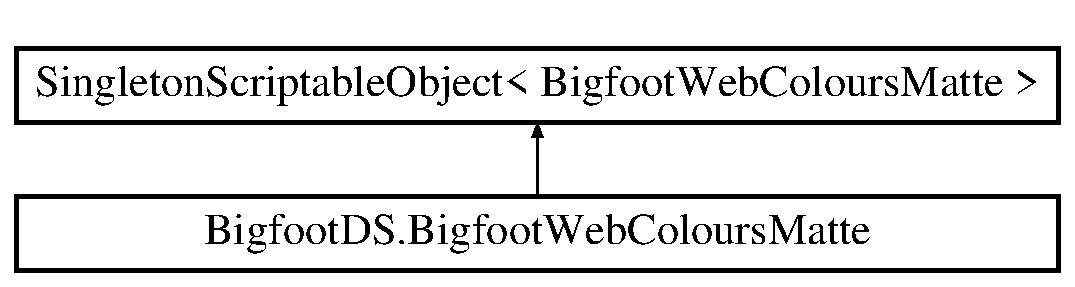
\includegraphics[height=2.000000cm]{class_bigfoot_d_s_1_1_bigfoot_web_colours_matte}
\end{center}
\end{figure}
\subsection*{Public Attributes}
\begin{DoxyCompactItemize}
\item 
\mbox{\Hypertarget{class_bigfoot_d_s_1_1_bigfoot_web_colours_matte_a08e4e5be93beb55fda8b9f48d58eb5bc}\label{class_bigfoot_d_s_1_1_bigfoot_web_colours_matte_a08e4e5be93beb55fda8b9f48d58eb5bc}} 
Material {\bfseries Alice\+Blue}
\item 
\mbox{\Hypertarget{class_bigfoot_d_s_1_1_bigfoot_web_colours_matte_a5ad28a76353265b40bcfba206fc6b695}\label{class_bigfoot_d_s_1_1_bigfoot_web_colours_matte_a5ad28a76353265b40bcfba206fc6b695}} 
Material {\bfseries Antique\+White}
\item 
\mbox{\Hypertarget{class_bigfoot_d_s_1_1_bigfoot_web_colours_matte_a86ede8fa607d2e11390014723cf79f20}\label{class_bigfoot_d_s_1_1_bigfoot_web_colours_matte_a86ede8fa607d2e11390014723cf79f20}} 
Material {\bfseries Aqua}
\item 
\mbox{\Hypertarget{class_bigfoot_d_s_1_1_bigfoot_web_colours_matte_a88cb2307e477a645f7ab20d45c53b599}\label{class_bigfoot_d_s_1_1_bigfoot_web_colours_matte_a88cb2307e477a645f7ab20d45c53b599}} 
Material {\bfseries Aquamarine}
\item 
\mbox{\Hypertarget{class_bigfoot_d_s_1_1_bigfoot_web_colours_matte_a2b4ffcf4f2bb9d371a452b7f81ee5acb}\label{class_bigfoot_d_s_1_1_bigfoot_web_colours_matte_a2b4ffcf4f2bb9d371a452b7f81ee5acb}} 
Material {\bfseries Azure}
\item 
\mbox{\Hypertarget{class_bigfoot_d_s_1_1_bigfoot_web_colours_matte_ab073106d611b406e1541bc083e2e3a05}\label{class_bigfoot_d_s_1_1_bigfoot_web_colours_matte_ab073106d611b406e1541bc083e2e3a05}} 
Material {\bfseries Beige}
\item 
\mbox{\Hypertarget{class_bigfoot_d_s_1_1_bigfoot_web_colours_matte_a38cdf0995ef81083569c8791657ae1b8}\label{class_bigfoot_d_s_1_1_bigfoot_web_colours_matte_a38cdf0995ef81083569c8791657ae1b8}} 
Material {\bfseries Bisque}
\item 
\mbox{\Hypertarget{class_bigfoot_d_s_1_1_bigfoot_web_colours_matte_a0334f4b2cb8cddc94c91bdb27b9db0f7}\label{class_bigfoot_d_s_1_1_bigfoot_web_colours_matte_a0334f4b2cb8cddc94c91bdb27b9db0f7}} 
Material {\bfseries Black}
\item 
\mbox{\Hypertarget{class_bigfoot_d_s_1_1_bigfoot_web_colours_matte_ab2d91c4d797c46a8aaa81e941f1a5539}\label{class_bigfoot_d_s_1_1_bigfoot_web_colours_matte_ab2d91c4d797c46a8aaa81e941f1a5539}} 
Material {\bfseries Blanched\+Almond}
\item 
\mbox{\Hypertarget{class_bigfoot_d_s_1_1_bigfoot_web_colours_matte_a3f008421fff29f1965344e8f63bb34f3}\label{class_bigfoot_d_s_1_1_bigfoot_web_colours_matte_a3f008421fff29f1965344e8f63bb34f3}} 
Material {\bfseries Blue}
\item 
\mbox{\Hypertarget{class_bigfoot_d_s_1_1_bigfoot_web_colours_matte_a9bb1a78d89a88edda0ad4249d69643da}\label{class_bigfoot_d_s_1_1_bigfoot_web_colours_matte_a9bb1a78d89a88edda0ad4249d69643da}} 
Material {\bfseries Blue\+Violet}
\item 
\mbox{\Hypertarget{class_bigfoot_d_s_1_1_bigfoot_web_colours_matte_a4a6ac4e27d8133e299f9a8db71ca105f}\label{class_bigfoot_d_s_1_1_bigfoot_web_colours_matte_a4a6ac4e27d8133e299f9a8db71ca105f}} 
Material {\bfseries Brown}
\item 
\mbox{\Hypertarget{class_bigfoot_d_s_1_1_bigfoot_web_colours_matte_a8c28681e5bee1222b8bfde510455f562}\label{class_bigfoot_d_s_1_1_bigfoot_web_colours_matte_a8c28681e5bee1222b8bfde510455f562}} 
Material {\bfseries Burly\+Wood}
\item 
\mbox{\Hypertarget{class_bigfoot_d_s_1_1_bigfoot_web_colours_matte_a27119e0f90da7fbaecd6c38102523a48}\label{class_bigfoot_d_s_1_1_bigfoot_web_colours_matte_a27119e0f90da7fbaecd6c38102523a48}} 
Material {\bfseries Cadet\+Blue}
\item 
\mbox{\Hypertarget{class_bigfoot_d_s_1_1_bigfoot_web_colours_matte_a2f59d04a4f12efe0612bcaa81acf133f}\label{class_bigfoot_d_s_1_1_bigfoot_web_colours_matte_a2f59d04a4f12efe0612bcaa81acf133f}} 
Material {\bfseries Chartreuse}
\item 
\mbox{\Hypertarget{class_bigfoot_d_s_1_1_bigfoot_web_colours_matte_af7aacdc2a68d5e7f2e3b843ea94ac7e8}\label{class_bigfoot_d_s_1_1_bigfoot_web_colours_matte_af7aacdc2a68d5e7f2e3b843ea94ac7e8}} 
Material {\bfseries Chocolate}
\item 
\mbox{\Hypertarget{class_bigfoot_d_s_1_1_bigfoot_web_colours_matte_af3512be1ca5b1e4d8698423ec0b740e5}\label{class_bigfoot_d_s_1_1_bigfoot_web_colours_matte_af3512be1ca5b1e4d8698423ec0b740e5}} 
Material {\bfseries Coral}
\item 
\mbox{\Hypertarget{class_bigfoot_d_s_1_1_bigfoot_web_colours_matte_a3e0f6c7f616789400f07a85580190e2c}\label{class_bigfoot_d_s_1_1_bigfoot_web_colours_matte_a3e0f6c7f616789400f07a85580190e2c}} 
Material {\bfseries Cornflower\+Blue}
\item 
\mbox{\Hypertarget{class_bigfoot_d_s_1_1_bigfoot_web_colours_matte_aafa75d25f25bfe17a7901489c64750ad}\label{class_bigfoot_d_s_1_1_bigfoot_web_colours_matte_aafa75d25f25bfe17a7901489c64750ad}} 
Material {\bfseries Cornsilk}
\item 
\mbox{\Hypertarget{class_bigfoot_d_s_1_1_bigfoot_web_colours_matte_a6b79a14ee3ce79bc4e64b8015e30831f}\label{class_bigfoot_d_s_1_1_bigfoot_web_colours_matte_a6b79a14ee3ce79bc4e64b8015e30831f}} 
Material {\bfseries Crimson}
\item 
\mbox{\Hypertarget{class_bigfoot_d_s_1_1_bigfoot_web_colours_matte_af30d16e32fbca74f793f0ad80277359c}\label{class_bigfoot_d_s_1_1_bigfoot_web_colours_matte_af30d16e32fbca74f793f0ad80277359c}} 
Material {\bfseries Cyan}
\item 
\mbox{\Hypertarget{class_bigfoot_d_s_1_1_bigfoot_web_colours_matte_ad9cbbf7bb20aaff083909e1a93baf6f5}\label{class_bigfoot_d_s_1_1_bigfoot_web_colours_matte_ad9cbbf7bb20aaff083909e1a93baf6f5}} 
Material {\bfseries Dark\+Blue}
\item 
\mbox{\Hypertarget{class_bigfoot_d_s_1_1_bigfoot_web_colours_matte_a24eb9b5604e5e64186f2b3e28932fcbf}\label{class_bigfoot_d_s_1_1_bigfoot_web_colours_matte_a24eb9b5604e5e64186f2b3e28932fcbf}} 
Material {\bfseries Dark\+Cyan}
\item 
\mbox{\Hypertarget{class_bigfoot_d_s_1_1_bigfoot_web_colours_matte_a86f77b88dee20abe666805c76a07d51e}\label{class_bigfoot_d_s_1_1_bigfoot_web_colours_matte_a86f77b88dee20abe666805c76a07d51e}} 
Material {\bfseries Dark\+Golden\+Rod}
\item 
\mbox{\Hypertarget{class_bigfoot_d_s_1_1_bigfoot_web_colours_matte_afa3ea81da2f3e2a3746c182d40b989db}\label{class_bigfoot_d_s_1_1_bigfoot_web_colours_matte_afa3ea81da2f3e2a3746c182d40b989db}} 
Material {\bfseries Dark\+Gray}
\item 
\mbox{\Hypertarget{class_bigfoot_d_s_1_1_bigfoot_web_colours_matte_aaf056320707de9362aeb1541874d214f}\label{class_bigfoot_d_s_1_1_bigfoot_web_colours_matte_aaf056320707de9362aeb1541874d214f}} 
Material {\bfseries Dark\+Grey}
\item 
\mbox{\Hypertarget{class_bigfoot_d_s_1_1_bigfoot_web_colours_matte_abde3c5736bdeb6cc7120563ec1d7de9b}\label{class_bigfoot_d_s_1_1_bigfoot_web_colours_matte_abde3c5736bdeb6cc7120563ec1d7de9b}} 
Material {\bfseries Dark\+Green}
\item 
\mbox{\Hypertarget{class_bigfoot_d_s_1_1_bigfoot_web_colours_matte_a46332b9976faf195a92e5fdba60586fa}\label{class_bigfoot_d_s_1_1_bigfoot_web_colours_matte_a46332b9976faf195a92e5fdba60586fa}} 
Material {\bfseries Dark\+Khaki}
\item 
\mbox{\Hypertarget{class_bigfoot_d_s_1_1_bigfoot_web_colours_matte_a005323225995be556b19ce3878ed67f1}\label{class_bigfoot_d_s_1_1_bigfoot_web_colours_matte_a005323225995be556b19ce3878ed67f1}} 
Material {\bfseries Dark\+Magenta}
\item 
\mbox{\Hypertarget{class_bigfoot_d_s_1_1_bigfoot_web_colours_matte_a7cec308fa6ec9c23490806d08c3b8a09}\label{class_bigfoot_d_s_1_1_bigfoot_web_colours_matte_a7cec308fa6ec9c23490806d08c3b8a09}} 
Material {\bfseries Dark\+Olive\+Green}
\item 
\mbox{\Hypertarget{class_bigfoot_d_s_1_1_bigfoot_web_colours_matte_a3a4730973cd53d4d2b1c6c521f6d372d}\label{class_bigfoot_d_s_1_1_bigfoot_web_colours_matte_a3a4730973cd53d4d2b1c6c521f6d372d}} 
Material {\bfseries Dark\+Orange}
\item 
\mbox{\Hypertarget{class_bigfoot_d_s_1_1_bigfoot_web_colours_matte_a0c5f83b919e4a3b88c7cb2c315de4d57}\label{class_bigfoot_d_s_1_1_bigfoot_web_colours_matte_a0c5f83b919e4a3b88c7cb2c315de4d57}} 
Material {\bfseries Dark\+Orchid}
\item 
\mbox{\Hypertarget{class_bigfoot_d_s_1_1_bigfoot_web_colours_matte_aa06388e03110284a0470a121edfc4173}\label{class_bigfoot_d_s_1_1_bigfoot_web_colours_matte_aa06388e03110284a0470a121edfc4173}} 
Material {\bfseries Dark\+Red}
\item 
\mbox{\Hypertarget{class_bigfoot_d_s_1_1_bigfoot_web_colours_matte_a8f4b6ce2d1d97c38d99ff19ce6cf86e4}\label{class_bigfoot_d_s_1_1_bigfoot_web_colours_matte_a8f4b6ce2d1d97c38d99ff19ce6cf86e4}} 
Material {\bfseries Dark\+Salmon}
\item 
\mbox{\Hypertarget{class_bigfoot_d_s_1_1_bigfoot_web_colours_matte_a81c81122ba882e1ed09c3bfacaa199f7}\label{class_bigfoot_d_s_1_1_bigfoot_web_colours_matte_a81c81122ba882e1ed09c3bfacaa199f7}} 
Material {\bfseries Dark\+Sea\+Green}
\item 
\mbox{\Hypertarget{class_bigfoot_d_s_1_1_bigfoot_web_colours_matte_aa4df454b4bd349a4aea9d9b0705a648c}\label{class_bigfoot_d_s_1_1_bigfoot_web_colours_matte_aa4df454b4bd349a4aea9d9b0705a648c}} 
Material {\bfseries Dark\+Slate\+Blue}
\item 
\mbox{\Hypertarget{class_bigfoot_d_s_1_1_bigfoot_web_colours_matte_a212f2eb7c4633f6706aa94bc692e2571}\label{class_bigfoot_d_s_1_1_bigfoot_web_colours_matte_a212f2eb7c4633f6706aa94bc692e2571}} 
Material {\bfseries Dark\+Slate\+Gray}
\item 
\mbox{\Hypertarget{class_bigfoot_d_s_1_1_bigfoot_web_colours_matte_a231d175279f3477956ec97f5f0d02c64}\label{class_bigfoot_d_s_1_1_bigfoot_web_colours_matte_a231d175279f3477956ec97f5f0d02c64}} 
Material {\bfseries Dark\+Slate\+Grey}
\item 
\mbox{\Hypertarget{class_bigfoot_d_s_1_1_bigfoot_web_colours_matte_a3d870a801cb018a882e6845466bcb214}\label{class_bigfoot_d_s_1_1_bigfoot_web_colours_matte_a3d870a801cb018a882e6845466bcb214}} 
Material {\bfseries Dark\+Turquoise}
\item 
\mbox{\Hypertarget{class_bigfoot_d_s_1_1_bigfoot_web_colours_matte_a3801f0008995349aa586bcefb5cbc4f2}\label{class_bigfoot_d_s_1_1_bigfoot_web_colours_matte_a3801f0008995349aa586bcefb5cbc4f2}} 
Material {\bfseries Dark\+Violet}
\item 
\mbox{\Hypertarget{class_bigfoot_d_s_1_1_bigfoot_web_colours_matte_a4cff59f0fbbb6987f8adaa7526bde9c7}\label{class_bigfoot_d_s_1_1_bigfoot_web_colours_matte_a4cff59f0fbbb6987f8adaa7526bde9c7}} 
Material {\bfseries Deep\+Pink}
\item 
\mbox{\Hypertarget{class_bigfoot_d_s_1_1_bigfoot_web_colours_matte_a0261c11e932a5513b7e849d3a0d613d5}\label{class_bigfoot_d_s_1_1_bigfoot_web_colours_matte_a0261c11e932a5513b7e849d3a0d613d5}} 
Material {\bfseries Deep\+Sky\+Blue}
\item 
\mbox{\Hypertarget{class_bigfoot_d_s_1_1_bigfoot_web_colours_matte_a4fe9e1f1f681d9ba1a9d512cdd3f66d5}\label{class_bigfoot_d_s_1_1_bigfoot_web_colours_matte_a4fe9e1f1f681d9ba1a9d512cdd3f66d5}} 
Material {\bfseries Dim\+Gray}
\item 
\mbox{\Hypertarget{class_bigfoot_d_s_1_1_bigfoot_web_colours_matte_a366cf765cbe1988a0b4cfff6b7fa5267}\label{class_bigfoot_d_s_1_1_bigfoot_web_colours_matte_a366cf765cbe1988a0b4cfff6b7fa5267}} 
Material {\bfseries Dim\+Grey}
\item 
\mbox{\Hypertarget{class_bigfoot_d_s_1_1_bigfoot_web_colours_matte_a9e5e3f920cb17c6c35dcc1836c1e4ab7}\label{class_bigfoot_d_s_1_1_bigfoot_web_colours_matte_a9e5e3f920cb17c6c35dcc1836c1e4ab7}} 
Material {\bfseries Dodger\+Blue}
\item 
\mbox{\Hypertarget{class_bigfoot_d_s_1_1_bigfoot_web_colours_matte_a34051d3d4c55f0c5cabf1858953c09a2}\label{class_bigfoot_d_s_1_1_bigfoot_web_colours_matte_a34051d3d4c55f0c5cabf1858953c09a2}} 
Material {\bfseries Fire\+Brick}
\item 
\mbox{\Hypertarget{class_bigfoot_d_s_1_1_bigfoot_web_colours_matte_afdcc5c3443ad488f15bcacd594355693}\label{class_bigfoot_d_s_1_1_bigfoot_web_colours_matte_afdcc5c3443ad488f15bcacd594355693}} 
Material {\bfseries Floral\+White}
\item 
\mbox{\Hypertarget{class_bigfoot_d_s_1_1_bigfoot_web_colours_matte_ac3685307236f65a01e6a2a1695f8ca24}\label{class_bigfoot_d_s_1_1_bigfoot_web_colours_matte_ac3685307236f65a01e6a2a1695f8ca24}} 
Material {\bfseries Forest\+Green}
\item 
\mbox{\Hypertarget{class_bigfoot_d_s_1_1_bigfoot_web_colours_matte_a361eb54483e8a994a6c80c715706ab03}\label{class_bigfoot_d_s_1_1_bigfoot_web_colours_matte_a361eb54483e8a994a6c80c715706ab03}} 
Material {\bfseries Fuchsia}
\item 
\mbox{\Hypertarget{class_bigfoot_d_s_1_1_bigfoot_web_colours_matte_af577bd5d6fa65dc43cb5c3d06bd3beac}\label{class_bigfoot_d_s_1_1_bigfoot_web_colours_matte_af577bd5d6fa65dc43cb5c3d06bd3beac}} 
Material {\bfseries Gainsboro}
\item 
\mbox{\Hypertarget{class_bigfoot_d_s_1_1_bigfoot_web_colours_matte_a3ec15d2c36389cddff889dd80e1d0893}\label{class_bigfoot_d_s_1_1_bigfoot_web_colours_matte_a3ec15d2c36389cddff889dd80e1d0893}} 
Material {\bfseries Ghost\+White}
\item 
\mbox{\Hypertarget{class_bigfoot_d_s_1_1_bigfoot_web_colours_matte_a0f327b6f845bcb645c3dc7649911f432}\label{class_bigfoot_d_s_1_1_bigfoot_web_colours_matte_a0f327b6f845bcb645c3dc7649911f432}} 
Material {\bfseries Gold}
\item 
\mbox{\Hypertarget{class_bigfoot_d_s_1_1_bigfoot_web_colours_matte_a15ead7e48d4e9246878e18b461075f42}\label{class_bigfoot_d_s_1_1_bigfoot_web_colours_matte_a15ead7e48d4e9246878e18b461075f42}} 
Material {\bfseries Golden\+Rod}
\item 
\mbox{\Hypertarget{class_bigfoot_d_s_1_1_bigfoot_web_colours_matte_a2837c3c631de8728ab2974fba2d3b8fc}\label{class_bigfoot_d_s_1_1_bigfoot_web_colours_matte_a2837c3c631de8728ab2974fba2d3b8fc}} 
Material {\bfseries Gray}
\item 
\mbox{\Hypertarget{class_bigfoot_d_s_1_1_bigfoot_web_colours_matte_a984516ccffd661fbd8e6f248faa94b4d}\label{class_bigfoot_d_s_1_1_bigfoot_web_colours_matte_a984516ccffd661fbd8e6f248faa94b4d}} 
Material {\bfseries Grey}
\item 
\mbox{\Hypertarget{class_bigfoot_d_s_1_1_bigfoot_web_colours_matte_a139ea5bffe4f38ab1ba278b9e83eaf42}\label{class_bigfoot_d_s_1_1_bigfoot_web_colours_matte_a139ea5bffe4f38ab1ba278b9e83eaf42}} 
Material {\bfseries Green}
\item 
\mbox{\Hypertarget{class_bigfoot_d_s_1_1_bigfoot_web_colours_matte_a4acf81410ea7aca3bbd62f3a34869414}\label{class_bigfoot_d_s_1_1_bigfoot_web_colours_matte_a4acf81410ea7aca3bbd62f3a34869414}} 
Material {\bfseries Green\+Yellow}
\item 
\mbox{\Hypertarget{class_bigfoot_d_s_1_1_bigfoot_web_colours_matte_a5fae153860211a7d687789391bb20af3}\label{class_bigfoot_d_s_1_1_bigfoot_web_colours_matte_a5fae153860211a7d687789391bb20af3}} 
Material {\bfseries Honey\+Dew}
\item 
\mbox{\Hypertarget{class_bigfoot_d_s_1_1_bigfoot_web_colours_matte_ae8d86ec376299450a38c2e6596bd9253}\label{class_bigfoot_d_s_1_1_bigfoot_web_colours_matte_ae8d86ec376299450a38c2e6596bd9253}} 
Material {\bfseries Hot\+Pink}
\item 
\mbox{\Hypertarget{class_bigfoot_d_s_1_1_bigfoot_web_colours_matte_a343270762db957bab901aa6b41250d09}\label{class_bigfoot_d_s_1_1_bigfoot_web_colours_matte_a343270762db957bab901aa6b41250d09}} 
Material {\bfseries Indian\+Red}
\item 
\mbox{\Hypertarget{class_bigfoot_d_s_1_1_bigfoot_web_colours_matte_af6259334e77532bb842a439840c2031a}\label{class_bigfoot_d_s_1_1_bigfoot_web_colours_matte_af6259334e77532bb842a439840c2031a}} 
Material {\bfseries Indigo}
\item 
\mbox{\Hypertarget{class_bigfoot_d_s_1_1_bigfoot_web_colours_matte_a474ae3f41ebca0ab1419cf2e57d74849}\label{class_bigfoot_d_s_1_1_bigfoot_web_colours_matte_a474ae3f41ebca0ab1419cf2e57d74849}} 
Material {\bfseries Ivory}
\item 
\mbox{\Hypertarget{class_bigfoot_d_s_1_1_bigfoot_web_colours_matte_a7825fc269dc301ecdf524bce2064d4e7}\label{class_bigfoot_d_s_1_1_bigfoot_web_colours_matte_a7825fc269dc301ecdf524bce2064d4e7}} 
Material {\bfseries Khaki}
\item 
\mbox{\Hypertarget{class_bigfoot_d_s_1_1_bigfoot_web_colours_matte_a98d5bb86f13456d86ff54227f37cd34b}\label{class_bigfoot_d_s_1_1_bigfoot_web_colours_matte_a98d5bb86f13456d86ff54227f37cd34b}} 
Material {\bfseries Lavender}
\item 
\mbox{\Hypertarget{class_bigfoot_d_s_1_1_bigfoot_web_colours_matte_ad24644041efa944f704005e288a35f54}\label{class_bigfoot_d_s_1_1_bigfoot_web_colours_matte_ad24644041efa944f704005e288a35f54}} 
Material {\bfseries Lavender\+Blush}
\item 
\mbox{\Hypertarget{class_bigfoot_d_s_1_1_bigfoot_web_colours_matte_a64c87f94991a504229c3441735f4363f}\label{class_bigfoot_d_s_1_1_bigfoot_web_colours_matte_a64c87f94991a504229c3441735f4363f}} 
Material {\bfseries Lawn\+Green}
\item 
\mbox{\Hypertarget{class_bigfoot_d_s_1_1_bigfoot_web_colours_matte_a802f6d152d80cd3ed4b7ecfdbdd5b048}\label{class_bigfoot_d_s_1_1_bigfoot_web_colours_matte_a802f6d152d80cd3ed4b7ecfdbdd5b048}} 
Material {\bfseries Lemon\+Chiffon}
\item 
\mbox{\Hypertarget{class_bigfoot_d_s_1_1_bigfoot_web_colours_matte_a79829e513973a08bd56906cc3df75892}\label{class_bigfoot_d_s_1_1_bigfoot_web_colours_matte_a79829e513973a08bd56906cc3df75892}} 
Material {\bfseries Light\+Blue}
\item 
\mbox{\Hypertarget{class_bigfoot_d_s_1_1_bigfoot_web_colours_matte_a69c22b5472a18c907d967f176adc0783}\label{class_bigfoot_d_s_1_1_bigfoot_web_colours_matte_a69c22b5472a18c907d967f176adc0783}} 
Material {\bfseries Light\+Coral}
\item 
\mbox{\Hypertarget{class_bigfoot_d_s_1_1_bigfoot_web_colours_matte_a8fbc1c6d0179ca0dc506b38362b3a3cf}\label{class_bigfoot_d_s_1_1_bigfoot_web_colours_matte_a8fbc1c6d0179ca0dc506b38362b3a3cf}} 
Material {\bfseries Light\+Cyan}
\item 
\mbox{\Hypertarget{class_bigfoot_d_s_1_1_bigfoot_web_colours_matte_a3d1848a4be948bd1c5a2af2fac7ff5af}\label{class_bigfoot_d_s_1_1_bigfoot_web_colours_matte_a3d1848a4be948bd1c5a2af2fac7ff5af}} 
Material {\bfseries Light\+Golden\+Rod\+Yellow}
\item 
\mbox{\Hypertarget{class_bigfoot_d_s_1_1_bigfoot_web_colours_matte_aaa2fb4bfe2f091aa69a2e5bef0da40f8}\label{class_bigfoot_d_s_1_1_bigfoot_web_colours_matte_aaa2fb4bfe2f091aa69a2e5bef0da40f8}} 
Material {\bfseries Light\+Gray}
\item 
\mbox{\Hypertarget{class_bigfoot_d_s_1_1_bigfoot_web_colours_matte_a3a06ba17c7733e22811811973f32451b}\label{class_bigfoot_d_s_1_1_bigfoot_web_colours_matte_a3a06ba17c7733e22811811973f32451b}} 
Material {\bfseries Light\+Grey}
\item 
\mbox{\Hypertarget{class_bigfoot_d_s_1_1_bigfoot_web_colours_matte_a4bd4bd569f1fedd91bf4dddd3456d51c}\label{class_bigfoot_d_s_1_1_bigfoot_web_colours_matte_a4bd4bd569f1fedd91bf4dddd3456d51c}} 
Material {\bfseries Light\+Green}
\item 
\mbox{\Hypertarget{class_bigfoot_d_s_1_1_bigfoot_web_colours_matte_a2b11500e86acd7e3c50020c53e93d591}\label{class_bigfoot_d_s_1_1_bigfoot_web_colours_matte_a2b11500e86acd7e3c50020c53e93d591}} 
Material {\bfseries Light\+Pink}
\item 
\mbox{\Hypertarget{class_bigfoot_d_s_1_1_bigfoot_web_colours_matte_a350e362f87726ca60de996796d25e325}\label{class_bigfoot_d_s_1_1_bigfoot_web_colours_matte_a350e362f87726ca60de996796d25e325}} 
Material {\bfseries Light\+Salmon}
\item 
\mbox{\Hypertarget{class_bigfoot_d_s_1_1_bigfoot_web_colours_matte_a267e75711733230ec383fa5bc0c37305}\label{class_bigfoot_d_s_1_1_bigfoot_web_colours_matte_a267e75711733230ec383fa5bc0c37305}} 
Material {\bfseries Light\+Sea\+Green}
\item 
\mbox{\Hypertarget{class_bigfoot_d_s_1_1_bigfoot_web_colours_matte_acf50075f19bc039cf5c91eebf6a22891}\label{class_bigfoot_d_s_1_1_bigfoot_web_colours_matte_acf50075f19bc039cf5c91eebf6a22891}} 
Material {\bfseries Light\+Sky\+Blue}
\item 
\mbox{\Hypertarget{class_bigfoot_d_s_1_1_bigfoot_web_colours_matte_aaf98d78272e4014eef2d794c124ae406}\label{class_bigfoot_d_s_1_1_bigfoot_web_colours_matte_aaf98d78272e4014eef2d794c124ae406}} 
Material {\bfseries Light\+Slate\+Gray}
\item 
\mbox{\Hypertarget{class_bigfoot_d_s_1_1_bigfoot_web_colours_matte_a80fad8a070f38fafb7473a2695e48aa0}\label{class_bigfoot_d_s_1_1_bigfoot_web_colours_matte_a80fad8a070f38fafb7473a2695e48aa0}} 
Material {\bfseries Light\+Slate\+Grey}
\item 
\mbox{\Hypertarget{class_bigfoot_d_s_1_1_bigfoot_web_colours_matte_aed4222bdcff2db20699e028e17f2b91e}\label{class_bigfoot_d_s_1_1_bigfoot_web_colours_matte_aed4222bdcff2db20699e028e17f2b91e}} 
Material {\bfseries Light\+Steel\+Blue}
\item 
\mbox{\Hypertarget{class_bigfoot_d_s_1_1_bigfoot_web_colours_matte_a5c2054ad72b920d7634ebcf8c23bd49f}\label{class_bigfoot_d_s_1_1_bigfoot_web_colours_matte_a5c2054ad72b920d7634ebcf8c23bd49f}} 
Material {\bfseries Light\+Yellow}
\item 
\mbox{\Hypertarget{class_bigfoot_d_s_1_1_bigfoot_web_colours_matte_a29d9c62650d58495070e49147015ebde}\label{class_bigfoot_d_s_1_1_bigfoot_web_colours_matte_a29d9c62650d58495070e49147015ebde}} 
Material {\bfseries Lime}
\item 
\mbox{\Hypertarget{class_bigfoot_d_s_1_1_bigfoot_web_colours_matte_a97d5203a0fad40f333b6584189210833}\label{class_bigfoot_d_s_1_1_bigfoot_web_colours_matte_a97d5203a0fad40f333b6584189210833}} 
Material {\bfseries Lime\+Green}
\item 
\mbox{\Hypertarget{class_bigfoot_d_s_1_1_bigfoot_web_colours_matte_a5a94d2069e41ef6db89c9777ff59d725}\label{class_bigfoot_d_s_1_1_bigfoot_web_colours_matte_a5a94d2069e41ef6db89c9777ff59d725}} 
Material {\bfseries Linen}
\item 
\mbox{\Hypertarget{class_bigfoot_d_s_1_1_bigfoot_web_colours_matte_aa086ecc6caad5b350eb8fc9cb4914390}\label{class_bigfoot_d_s_1_1_bigfoot_web_colours_matte_aa086ecc6caad5b350eb8fc9cb4914390}} 
Material {\bfseries Magenta}
\item 
\mbox{\Hypertarget{class_bigfoot_d_s_1_1_bigfoot_web_colours_matte_afdc338ce5d213cf34396111b44bf5d7c}\label{class_bigfoot_d_s_1_1_bigfoot_web_colours_matte_afdc338ce5d213cf34396111b44bf5d7c}} 
Material {\bfseries Maroon}
\item 
\mbox{\Hypertarget{class_bigfoot_d_s_1_1_bigfoot_web_colours_matte_ac3ab0fb97cbd9f28f0e25165d065b333}\label{class_bigfoot_d_s_1_1_bigfoot_web_colours_matte_ac3ab0fb97cbd9f28f0e25165d065b333}} 
Material {\bfseries Medium\+Aqua\+Marine}
\item 
\mbox{\Hypertarget{class_bigfoot_d_s_1_1_bigfoot_web_colours_matte_abb15cd24a891140eafba434e6cc3d35e}\label{class_bigfoot_d_s_1_1_bigfoot_web_colours_matte_abb15cd24a891140eafba434e6cc3d35e}} 
Material {\bfseries Medium\+Blue}
\item 
\mbox{\Hypertarget{class_bigfoot_d_s_1_1_bigfoot_web_colours_matte_ad480d7be9c76d11f6256c0aa666a92e5}\label{class_bigfoot_d_s_1_1_bigfoot_web_colours_matte_ad480d7be9c76d11f6256c0aa666a92e5}} 
Material {\bfseries Medium\+Orchid}
\item 
\mbox{\Hypertarget{class_bigfoot_d_s_1_1_bigfoot_web_colours_matte_ad7d6b5e7e5e579497a91bf46be923f37}\label{class_bigfoot_d_s_1_1_bigfoot_web_colours_matte_ad7d6b5e7e5e579497a91bf46be923f37}} 
Material {\bfseries Medium\+Purple}
\item 
\mbox{\Hypertarget{class_bigfoot_d_s_1_1_bigfoot_web_colours_matte_add62a4a494844d3368a39634b94d1fbe}\label{class_bigfoot_d_s_1_1_bigfoot_web_colours_matte_add62a4a494844d3368a39634b94d1fbe}} 
Material {\bfseries Medium\+Sea\+Green}
\item 
\mbox{\Hypertarget{class_bigfoot_d_s_1_1_bigfoot_web_colours_matte_add189cea9b72f15378139bdb4289417a}\label{class_bigfoot_d_s_1_1_bigfoot_web_colours_matte_add189cea9b72f15378139bdb4289417a}} 
Material {\bfseries Medium\+Slate\+Blue}
\item 
\mbox{\Hypertarget{class_bigfoot_d_s_1_1_bigfoot_web_colours_matte_af2b8a362d8563bcb6e9ac4c5cf6b1f74}\label{class_bigfoot_d_s_1_1_bigfoot_web_colours_matte_af2b8a362d8563bcb6e9ac4c5cf6b1f74}} 
Material {\bfseries Medium\+Spring\+Green}
\item 
\mbox{\Hypertarget{class_bigfoot_d_s_1_1_bigfoot_web_colours_matte_a24592e281370d111d29f18a4bff0d4fd}\label{class_bigfoot_d_s_1_1_bigfoot_web_colours_matte_a24592e281370d111d29f18a4bff0d4fd}} 
Material {\bfseries Medium\+Turquoise}
\item 
\mbox{\Hypertarget{class_bigfoot_d_s_1_1_bigfoot_web_colours_matte_aa52a769115b1097f3f74c2b92af8427c}\label{class_bigfoot_d_s_1_1_bigfoot_web_colours_matte_aa52a769115b1097f3f74c2b92af8427c}} 
Material {\bfseries Medium\+Violet\+Red}
\item 
\mbox{\Hypertarget{class_bigfoot_d_s_1_1_bigfoot_web_colours_matte_a4686d9177bba2d7639bf1f962aa413eb}\label{class_bigfoot_d_s_1_1_bigfoot_web_colours_matte_a4686d9177bba2d7639bf1f962aa413eb}} 
Material {\bfseries Midnight\+Blue}
\item 
\mbox{\Hypertarget{class_bigfoot_d_s_1_1_bigfoot_web_colours_matte_ac38f0d6db3d99cbc852b23da481fb261}\label{class_bigfoot_d_s_1_1_bigfoot_web_colours_matte_ac38f0d6db3d99cbc852b23da481fb261}} 
Material {\bfseries Mint\+Cream}
\item 
\mbox{\Hypertarget{class_bigfoot_d_s_1_1_bigfoot_web_colours_matte_a4ed2a22683b99da45021d08a5eba98b0}\label{class_bigfoot_d_s_1_1_bigfoot_web_colours_matte_a4ed2a22683b99da45021d08a5eba98b0}} 
Material {\bfseries Misty\+Rose}
\item 
\mbox{\Hypertarget{class_bigfoot_d_s_1_1_bigfoot_web_colours_matte_aa0c9687afa4da81c5ef710cad115d918}\label{class_bigfoot_d_s_1_1_bigfoot_web_colours_matte_aa0c9687afa4da81c5ef710cad115d918}} 
Material {\bfseries Moccasin}
\item 
\mbox{\Hypertarget{class_bigfoot_d_s_1_1_bigfoot_web_colours_matte_a195c866015e77e51fd470f2303caaa2b}\label{class_bigfoot_d_s_1_1_bigfoot_web_colours_matte_a195c866015e77e51fd470f2303caaa2b}} 
Material {\bfseries Navajo\+White}
\item 
\mbox{\Hypertarget{class_bigfoot_d_s_1_1_bigfoot_web_colours_matte_aa8931533521e473b605df7dd2d61185b}\label{class_bigfoot_d_s_1_1_bigfoot_web_colours_matte_aa8931533521e473b605df7dd2d61185b}} 
Material {\bfseries Navy}
\item 
\mbox{\Hypertarget{class_bigfoot_d_s_1_1_bigfoot_web_colours_matte_aab36f2f80b03b18a44e2383a104e0692}\label{class_bigfoot_d_s_1_1_bigfoot_web_colours_matte_aab36f2f80b03b18a44e2383a104e0692}} 
Material {\bfseries Old\+Lace}
\item 
\mbox{\Hypertarget{class_bigfoot_d_s_1_1_bigfoot_web_colours_matte_add355a2be0cad88fc1f7fa5f073f9c9f}\label{class_bigfoot_d_s_1_1_bigfoot_web_colours_matte_add355a2be0cad88fc1f7fa5f073f9c9f}} 
Material {\bfseries Olive}
\item 
\mbox{\Hypertarget{class_bigfoot_d_s_1_1_bigfoot_web_colours_matte_a7c08bd920882803a23e49229c37b052a}\label{class_bigfoot_d_s_1_1_bigfoot_web_colours_matte_a7c08bd920882803a23e49229c37b052a}} 
Material {\bfseries Olive\+Drab}
\item 
\mbox{\Hypertarget{class_bigfoot_d_s_1_1_bigfoot_web_colours_matte_a82e355cd6c43579082a2919dd148a961}\label{class_bigfoot_d_s_1_1_bigfoot_web_colours_matte_a82e355cd6c43579082a2919dd148a961}} 
Material {\bfseries Orange}
\item 
\mbox{\Hypertarget{class_bigfoot_d_s_1_1_bigfoot_web_colours_matte_a5d745d579334fa08a2b0ee037b1b954c}\label{class_bigfoot_d_s_1_1_bigfoot_web_colours_matte_a5d745d579334fa08a2b0ee037b1b954c}} 
Material {\bfseries Orange\+Red}
\item 
\mbox{\Hypertarget{class_bigfoot_d_s_1_1_bigfoot_web_colours_matte_ab3117db34a3e5b71ac74580fbaba28b0}\label{class_bigfoot_d_s_1_1_bigfoot_web_colours_matte_ab3117db34a3e5b71ac74580fbaba28b0}} 
Material {\bfseries Orchid}
\item 
\mbox{\Hypertarget{class_bigfoot_d_s_1_1_bigfoot_web_colours_matte_a486359f6a256e99bbbf36b6cfb0e95bb}\label{class_bigfoot_d_s_1_1_bigfoot_web_colours_matte_a486359f6a256e99bbbf36b6cfb0e95bb}} 
Material {\bfseries Pale\+Golden\+Rod}
\item 
\mbox{\Hypertarget{class_bigfoot_d_s_1_1_bigfoot_web_colours_matte_a06f18022e869728b56b45a92c5a9960b}\label{class_bigfoot_d_s_1_1_bigfoot_web_colours_matte_a06f18022e869728b56b45a92c5a9960b}} 
Material {\bfseries Pale\+Green}
\item 
\mbox{\Hypertarget{class_bigfoot_d_s_1_1_bigfoot_web_colours_matte_a7bd957618bc2627939620bb19942a0ee}\label{class_bigfoot_d_s_1_1_bigfoot_web_colours_matte_a7bd957618bc2627939620bb19942a0ee}} 
Material {\bfseries Pale\+Turquoise}
\item 
\mbox{\Hypertarget{class_bigfoot_d_s_1_1_bigfoot_web_colours_matte_a1d3f4610cd3706ee3dc797e3a84506d4}\label{class_bigfoot_d_s_1_1_bigfoot_web_colours_matte_a1d3f4610cd3706ee3dc797e3a84506d4}} 
Material {\bfseries Pale\+Violet\+Red}
\item 
\mbox{\Hypertarget{class_bigfoot_d_s_1_1_bigfoot_web_colours_matte_a7d687e8ec33aff83fb415b6b6bddb3aa}\label{class_bigfoot_d_s_1_1_bigfoot_web_colours_matte_a7d687e8ec33aff83fb415b6b6bddb3aa}} 
Material {\bfseries Papaya\+Whip}
\item 
\mbox{\Hypertarget{class_bigfoot_d_s_1_1_bigfoot_web_colours_matte_ab9338c8e8adb62cfdcd62b0a37c4ffe6}\label{class_bigfoot_d_s_1_1_bigfoot_web_colours_matte_ab9338c8e8adb62cfdcd62b0a37c4ffe6}} 
Material {\bfseries Peach\+Puff}
\item 
\mbox{\Hypertarget{class_bigfoot_d_s_1_1_bigfoot_web_colours_matte_adc9e703da92bbff7534c9822e5b0f4a5}\label{class_bigfoot_d_s_1_1_bigfoot_web_colours_matte_adc9e703da92bbff7534c9822e5b0f4a5}} 
Material {\bfseries Peru}
\item 
\mbox{\Hypertarget{class_bigfoot_d_s_1_1_bigfoot_web_colours_matte_aea8edbbad7e0919f5450ddd615224633}\label{class_bigfoot_d_s_1_1_bigfoot_web_colours_matte_aea8edbbad7e0919f5450ddd615224633}} 
Material {\bfseries Pink}
\item 
\mbox{\Hypertarget{class_bigfoot_d_s_1_1_bigfoot_web_colours_matte_ad8dfda258072e71580144ebe37b1b635}\label{class_bigfoot_d_s_1_1_bigfoot_web_colours_matte_ad8dfda258072e71580144ebe37b1b635}} 
Material {\bfseries Plum}
\item 
\mbox{\Hypertarget{class_bigfoot_d_s_1_1_bigfoot_web_colours_matte_a2dffcec756760040d737f8e310216869}\label{class_bigfoot_d_s_1_1_bigfoot_web_colours_matte_a2dffcec756760040d737f8e310216869}} 
Material {\bfseries Powder\+Blue}
\item 
\mbox{\Hypertarget{class_bigfoot_d_s_1_1_bigfoot_web_colours_matte_a72450c7a08f7fb390a5d341af1ffaf43}\label{class_bigfoot_d_s_1_1_bigfoot_web_colours_matte_a72450c7a08f7fb390a5d341af1ffaf43}} 
Material {\bfseries Purple}
\item 
\mbox{\Hypertarget{class_bigfoot_d_s_1_1_bigfoot_web_colours_matte_a385b0b8801f64140b49f1222751d033d}\label{class_bigfoot_d_s_1_1_bigfoot_web_colours_matte_a385b0b8801f64140b49f1222751d033d}} 
Material {\bfseries Rebecca\+Purple}
\item 
\mbox{\Hypertarget{class_bigfoot_d_s_1_1_bigfoot_web_colours_matte_a5fa1d15cf806995cd0c4a5fdb446bfa5}\label{class_bigfoot_d_s_1_1_bigfoot_web_colours_matte_a5fa1d15cf806995cd0c4a5fdb446bfa5}} 
Material {\bfseries Red}
\item 
\mbox{\Hypertarget{class_bigfoot_d_s_1_1_bigfoot_web_colours_matte_a89fa41b30c4a3cd453800e64ba595687}\label{class_bigfoot_d_s_1_1_bigfoot_web_colours_matte_a89fa41b30c4a3cd453800e64ba595687}} 
Material {\bfseries Rosy\+Brown}
\item 
\mbox{\Hypertarget{class_bigfoot_d_s_1_1_bigfoot_web_colours_matte_a79ee9a6ff5457b5e0f858df391f86e03}\label{class_bigfoot_d_s_1_1_bigfoot_web_colours_matte_a79ee9a6ff5457b5e0f858df391f86e03}} 
Material {\bfseries Royal\+Blue}
\item 
\mbox{\Hypertarget{class_bigfoot_d_s_1_1_bigfoot_web_colours_matte_aa6a83fddcaaf64b8fc52cf89c6aaec18}\label{class_bigfoot_d_s_1_1_bigfoot_web_colours_matte_aa6a83fddcaaf64b8fc52cf89c6aaec18}} 
Material {\bfseries Saddle\+Brown}
\item 
\mbox{\Hypertarget{class_bigfoot_d_s_1_1_bigfoot_web_colours_matte_ab38b09e53c72008e534d03d416de4487}\label{class_bigfoot_d_s_1_1_bigfoot_web_colours_matte_ab38b09e53c72008e534d03d416de4487}} 
Material {\bfseries Salmon}
\item 
\mbox{\Hypertarget{class_bigfoot_d_s_1_1_bigfoot_web_colours_matte_a3ee93ad9cd07663c459f18f27464d049}\label{class_bigfoot_d_s_1_1_bigfoot_web_colours_matte_a3ee93ad9cd07663c459f18f27464d049}} 
Material {\bfseries Sandy\+Brown}
\item 
\mbox{\Hypertarget{class_bigfoot_d_s_1_1_bigfoot_web_colours_matte_a5975517818a3d1a95b5953ef45bf8ac8}\label{class_bigfoot_d_s_1_1_bigfoot_web_colours_matte_a5975517818a3d1a95b5953ef45bf8ac8}} 
Material {\bfseries Sea\+Green}
\item 
\mbox{\Hypertarget{class_bigfoot_d_s_1_1_bigfoot_web_colours_matte_a14fd3d38424785caa547cb5406c5612b}\label{class_bigfoot_d_s_1_1_bigfoot_web_colours_matte_a14fd3d38424785caa547cb5406c5612b}} 
Material {\bfseries Sea\+Shell}
\item 
\mbox{\Hypertarget{class_bigfoot_d_s_1_1_bigfoot_web_colours_matte_a08616d1e0d6ad5a15b660b796d1f6356}\label{class_bigfoot_d_s_1_1_bigfoot_web_colours_matte_a08616d1e0d6ad5a15b660b796d1f6356}} 
Material {\bfseries Sienna}
\item 
\mbox{\Hypertarget{class_bigfoot_d_s_1_1_bigfoot_web_colours_matte_abacb7ccf9ba8cbdd61c261df190ac816}\label{class_bigfoot_d_s_1_1_bigfoot_web_colours_matte_abacb7ccf9ba8cbdd61c261df190ac816}} 
Material {\bfseries Silver}
\item 
\mbox{\Hypertarget{class_bigfoot_d_s_1_1_bigfoot_web_colours_matte_a4afd01c4b5d082a8905a532dddae3806}\label{class_bigfoot_d_s_1_1_bigfoot_web_colours_matte_a4afd01c4b5d082a8905a532dddae3806}} 
Material {\bfseries Sky\+Blue}
\item 
\mbox{\Hypertarget{class_bigfoot_d_s_1_1_bigfoot_web_colours_matte_ada165eb537dd2e4517769f6f37834fc5}\label{class_bigfoot_d_s_1_1_bigfoot_web_colours_matte_ada165eb537dd2e4517769f6f37834fc5}} 
Material {\bfseries Slate\+Blue}
\item 
\mbox{\Hypertarget{class_bigfoot_d_s_1_1_bigfoot_web_colours_matte_ab0dd622819815d517d6dd2e97d703937}\label{class_bigfoot_d_s_1_1_bigfoot_web_colours_matte_ab0dd622819815d517d6dd2e97d703937}} 
Material {\bfseries Slate\+Gray}
\item 
\mbox{\Hypertarget{class_bigfoot_d_s_1_1_bigfoot_web_colours_matte_a2773792712fd8f4e6f616509f773dc64}\label{class_bigfoot_d_s_1_1_bigfoot_web_colours_matte_a2773792712fd8f4e6f616509f773dc64}} 
Material {\bfseries Slate\+Grey}
\item 
\mbox{\Hypertarget{class_bigfoot_d_s_1_1_bigfoot_web_colours_matte_a4c0b1b3af8c219a68cad71c48ca39277}\label{class_bigfoot_d_s_1_1_bigfoot_web_colours_matte_a4c0b1b3af8c219a68cad71c48ca39277}} 
Material {\bfseries Snow}
\item 
\mbox{\Hypertarget{class_bigfoot_d_s_1_1_bigfoot_web_colours_matte_aca05fd938fd832f3c74935084f287094}\label{class_bigfoot_d_s_1_1_bigfoot_web_colours_matte_aca05fd938fd832f3c74935084f287094}} 
Material {\bfseries Spring\+Green}
\item 
\mbox{\Hypertarget{class_bigfoot_d_s_1_1_bigfoot_web_colours_matte_a42619eae12bc5c50e6af7ccc5d54eb5b}\label{class_bigfoot_d_s_1_1_bigfoot_web_colours_matte_a42619eae12bc5c50e6af7ccc5d54eb5b}} 
Material {\bfseries Steel\+Blue}
\item 
\mbox{\Hypertarget{class_bigfoot_d_s_1_1_bigfoot_web_colours_matte_af738f799b4fd3149b4c4f0cad81a28df}\label{class_bigfoot_d_s_1_1_bigfoot_web_colours_matte_af738f799b4fd3149b4c4f0cad81a28df}} 
Material {\bfseries Tan}
\item 
\mbox{\Hypertarget{class_bigfoot_d_s_1_1_bigfoot_web_colours_matte_a3258951736124e1db5f91f57d4ee288a}\label{class_bigfoot_d_s_1_1_bigfoot_web_colours_matte_a3258951736124e1db5f91f57d4ee288a}} 
Material {\bfseries Teal}
\item 
\mbox{\Hypertarget{class_bigfoot_d_s_1_1_bigfoot_web_colours_matte_a09597dec61b49e2a2714c88d03c3c23d}\label{class_bigfoot_d_s_1_1_bigfoot_web_colours_matte_a09597dec61b49e2a2714c88d03c3c23d}} 
Material {\bfseries Thistle}
\item 
\mbox{\Hypertarget{class_bigfoot_d_s_1_1_bigfoot_web_colours_matte_ae16d8af4de6495cd8e3e28f23b21c976}\label{class_bigfoot_d_s_1_1_bigfoot_web_colours_matte_ae16d8af4de6495cd8e3e28f23b21c976}} 
Material {\bfseries Tomato}
\item 
\mbox{\Hypertarget{class_bigfoot_d_s_1_1_bigfoot_web_colours_matte_a3423d04b235f3e4c54ebdbe96d596e07}\label{class_bigfoot_d_s_1_1_bigfoot_web_colours_matte_a3423d04b235f3e4c54ebdbe96d596e07}} 
Material {\bfseries Turquoise}
\item 
\mbox{\Hypertarget{class_bigfoot_d_s_1_1_bigfoot_web_colours_matte_acc51d8b77d2b2588790d74f5505d8580}\label{class_bigfoot_d_s_1_1_bigfoot_web_colours_matte_acc51d8b77d2b2588790d74f5505d8580}} 
Material {\bfseries Violet}
\item 
\mbox{\Hypertarget{class_bigfoot_d_s_1_1_bigfoot_web_colours_matte_a8f825fa467a990ea3ec3bebc2998c91b}\label{class_bigfoot_d_s_1_1_bigfoot_web_colours_matte_a8f825fa467a990ea3ec3bebc2998c91b}} 
Material {\bfseries Wheat}
\item 
\mbox{\Hypertarget{class_bigfoot_d_s_1_1_bigfoot_web_colours_matte_a3c86726cb4fd8f4b314058d5db5c5ae8}\label{class_bigfoot_d_s_1_1_bigfoot_web_colours_matte_a3c86726cb4fd8f4b314058d5db5c5ae8}} 
Material {\bfseries White}
\item 
\mbox{\Hypertarget{class_bigfoot_d_s_1_1_bigfoot_web_colours_matte_a43d540fe222ba06bcc58f0d40bb71125}\label{class_bigfoot_d_s_1_1_bigfoot_web_colours_matte_a43d540fe222ba06bcc58f0d40bb71125}} 
Material {\bfseries White\+Smoke}
\item 
\mbox{\Hypertarget{class_bigfoot_d_s_1_1_bigfoot_web_colours_matte_a1552a72f547e626f83d5b3c967f96512}\label{class_bigfoot_d_s_1_1_bigfoot_web_colours_matte_a1552a72f547e626f83d5b3c967f96512}} 
Material {\bfseries Yellow}
\item 
\mbox{\Hypertarget{class_bigfoot_d_s_1_1_bigfoot_web_colours_matte_a5b7837231fca86af557ceb63473b7103}\label{class_bigfoot_d_s_1_1_bigfoot_web_colours_matte_a5b7837231fca86af557ceb63473b7103}} 
Material {\bfseries Yellow\+Green}
\item 
\mbox{\Hypertarget{class_bigfoot_d_s_1_1_bigfoot_web_colours_matte_af54f35ef94926411c7fa8469ec8ce664}\label{class_bigfoot_d_s_1_1_bigfoot_web_colours_matte_af54f35ef94926411c7fa8469ec8ce664}} 
List$<$ Material $>$ {\bfseries materials\+Matte}
\end{DoxyCompactItemize}
\subsection*{Additional Inherited Members}


The documentation for this class was generated from the following file\+:\begin{DoxyCompactItemize}
\item 
Assets/\+Bigfoot\+D\+S/\+\_\+\+Common/\+Scripts/Bigfoot\+Web\+Colours\+Matte.\+cs\end{DoxyCompactItemize}

\hypertarget{class_bigfoot_d_s_1_1_bigfoot_web_colours_metallic}{}\section{Bigfoot\+D\+S.\+Bigfoot\+Web\+Colours\+Metallic Class Reference}
\label{class_bigfoot_d_s_1_1_bigfoot_web_colours_metallic}\index{Bigfoot\+D\+S.\+Bigfoot\+Web\+Colours\+Metallic@{Bigfoot\+D\+S.\+Bigfoot\+Web\+Colours\+Metallic}}
Inheritance diagram for Bigfoot\+D\+S.\+Bigfoot\+Web\+Colours\+Metallic\+:\begin{figure}[H]
\begin{center}
\leavevmode
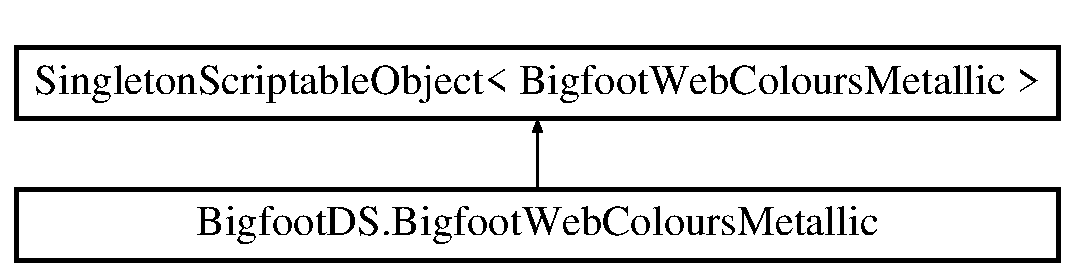
\includegraphics[height=2.000000cm]{class_bigfoot_d_s_1_1_bigfoot_web_colours_metallic}
\end{center}
\end{figure}
\subsection*{Public Attributes}
\begin{DoxyCompactItemize}
\item 
\mbox{\Hypertarget{class_bigfoot_d_s_1_1_bigfoot_web_colours_metallic_a8a86cc25741cfa45a05c02b93039ce69}\label{class_bigfoot_d_s_1_1_bigfoot_web_colours_metallic_a8a86cc25741cfa45a05c02b93039ce69}} 
Material {\bfseries Alice\+Blue}
\item 
\mbox{\Hypertarget{class_bigfoot_d_s_1_1_bigfoot_web_colours_metallic_ae495d9401b613473f5e03dd001e343d2}\label{class_bigfoot_d_s_1_1_bigfoot_web_colours_metallic_ae495d9401b613473f5e03dd001e343d2}} 
Material {\bfseries Antique\+White}
\item 
\mbox{\Hypertarget{class_bigfoot_d_s_1_1_bigfoot_web_colours_metallic_ae2a33a631078ce8899c5ce242f067c56}\label{class_bigfoot_d_s_1_1_bigfoot_web_colours_metallic_ae2a33a631078ce8899c5ce242f067c56}} 
Material {\bfseries Aqua}
\item 
\mbox{\Hypertarget{class_bigfoot_d_s_1_1_bigfoot_web_colours_metallic_a7c02c11bd0ecf2b5376b6d62dd185124}\label{class_bigfoot_d_s_1_1_bigfoot_web_colours_metallic_a7c02c11bd0ecf2b5376b6d62dd185124}} 
Material {\bfseries Aquamarine}
\item 
\mbox{\Hypertarget{class_bigfoot_d_s_1_1_bigfoot_web_colours_metallic_a0bfcc8e89a521e7085355b379b91e358}\label{class_bigfoot_d_s_1_1_bigfoot_web_colours_metallic_a0bfcc8e89a521e7085355b379b91e358}} 
Material {\bfseries Azure}
\item 
\mbox{\Hypertarget{class_bigfoot_d_s_1_1_bigfoot_web_colours_metallic_ad99b32c4f057e10d2a11cd1612414a91}\label{class_bigfoot_d_s_1_1_bigfoot_web_colours_metallic_ad99b32c4f057e10d2a11cd1612414a91}} 
Material {\bfseries Beige}
\item 
\mbox{\Hypertarget{class_bigfoot_d_s_1_1_bigfoot_web_colours_metallic_aeb4f8f4f83ab93ef8f74bcc8a0efc1bd}\label{class_bigfoot_d_s_1_1_bigfoot_web_colours_metallic_aeb4f8f4f83ab93ef8f74bcc8a0efc1bd}} 
Material {\bfseries Bisque}
\item 
\mbox{\Hypertarget{class_bigfoot_d_s_1_1_bigfoot_web_colours_metallic_a9cd05062dca197df4991e11ade81a763}\label{class_bigfoot_d_s_1_1_bigfoot_web_colours_metallic_a9cd05062dca197df4991e11ade81a763}} 
Material {\bfseries Black}
\item 
\mbox{\Hypertarget{class_bigfoot_d_s_1_1_bigfoot_web_colours_metallic_a5c0b7487cd94e7bfd1d9647e0dc8f0ee}\label{class_bigfoot_d_s_1_1_bigfoot_web_colours_metallic_a5c0b7487cd94e7bfd1d9647e0dc8f0ee}} 
Material {\bfseries Blanched\+Almond}
\item 
\mbox{\Hypertarget{class_bigfoot_d_s_1_1_bigfoot_web_colours_metallic_a687fbca286d626b3d68c393ee852607c}\label{class_bigfoot_d_s_1_1_bigfoot_web_colours_metallic_a687fbca286d626b3d68c393ee852607c}} 
Material {\bfseries Blue}
\item 
\mbox{\Hypertarget{class_bigfoot_d_s_1_1_bigfoot_web_colours_metallic_a7ce01480587ad4bd17b489017757013a}\label{class_bigfoot_d_s_1_1_bigfoot_web_colours_metallic_a7ce01480587ad4bd17b489017757013a}} 
Material {\bfseries Blue\+Violet}
\item 
\mbox{\Hypertarget{class_bigfoot_d_s_1_1_bigfoot_web_colours_metallic_a201655e0ad24269970fd7aeff0e77d03}\label{class_bigfoot_d_s_1_1_bigfoot_web_colours_metallic_a201655e0ad24269970fd7aeff0e77d03}} 
Material {\bfseries Brown}
\item 
\mbox{\Hypertarget{class_bigfoot_d_s_1_1_bigfoot_web_colours_metallic_aa50bd49a2a5ec95bccf2b3a07a7d12d7}\label{class_bigfoot_d_s_1_1_bigfoot_web_colours_metallic_aa50bd49a2a5ec95bccf2b3a07a7d12d7}} 
Material {\bfseries Burly\+Wood}
\item 
\mbox{\Hypertarget{class_bigfoot_d_s_1_1_bigfoot_web_colours_metallic_a98ed9f911c2806214c82e4cd55d3e9f4}\label{class_bigfoot_d_s_1_1_bigfoot_web_colours_metallic_a98ed9f911c2806214c82e4cd55d3e9f4}} 
Material {\bfseries Cadet\+Blue}
\item 
\mbox{\Hypertarget{class_bigfoot_d_s_1_1_bigfoot_web_colours_metallic_a27e30c4a0ba9d70516900fc4f4563db4}\label{class_bigfoot_d_s_1_1_bigfoot_web_colours_metallic_a27e30c4a0ba9d70516900fc4f4563db4}} 
Material {\bfseries Chartreuse}
\item 
\mbox{\Hypertarget{class_bigfoot_d_s_1_1_bigfoot_web_colours_metallic_a6c7f6b90b6ea33a90395f2d30383b2b7}\label{class_bigfoot_d_s_1_1_bigfoot_web_colours_metallic_a6c7f6b90b6ea33a90395f2d30383b2b7}} 
Material {\bfseries Chocolate}
\item 
\mbox{\Hypertarget{class_bigfoot_d_s_1_1_bigfoot_web_colours_metallic_ade54e17bfb1547dd463c60bf1663c5ff}\label{class_bigfoot_d_s_1_1_bigfoot_web_colours_metallic_ade54e17bfb1547dd463c60bf1663c5ff}} 
Material {\bfseries Coral}
\item 
\mbox{\Hypertarget{class_bigfoot_d_s_1_1_bigfoot_web_colours_metallic_a505bacf96b7439e116806ffeec5999bf}\label{class_bigfoot_d_s_1_1_bigfoot_web_colours_metallic_a505bacf96b7439e116806ffeec5999bf}} 
Material {\bfseries Cornflower\+Blue}
\item 
\mbox{\Hypertarget{class_bigfoot_d_s_1_1_bigfoot_web_colours_metallic_a415f80251d3ed82630c4ae1806aa6edc}\label{class_bigfoot_d_s_1_1_bigfoot_web_colours_metallic_a415f80251d3ed82630c4ae1806aa6edc}} 
Material {\bfseries Cornsilk}
\item 
\mbox{\Hypertarget{class_bigfoot_d_s_1_1_bigfoot_web_colours_metallic_a5745ca643396d263be65ad33a009febb}\label{class_bigfoot_d_s_1_1_bigfoot_web_colours_metallic_a5745ca643396d263be65ad33a009febb}} 
Material {\bfseries Crimson}
\item 
\mbox{\Hypertarget{class_bigfoot_d_s_1_1_bigfoot_web_colours_metallic_aaa9020eab56f70005cc452bedabedee7}\label{class_bigfoot_d_s_1_1_bigfoot_web_colours_metallic_aaa9020eab56f70005cc452bedabedee7}} 
Material {\bfseries Cyan}
\item 
\mbox{\Hypertarget{class_bigfoot_d_s_1_1_bigfoot_web_colours_metallic_a8aa84e7c938a0f75cabb27598d298a0b}\label{class_bigfoot_d_s_1_1_bigfoot_web_colours_metallic_a8aa84e7c938a0f75cabb27598d298a0b}} 
Material {\bfseries Dark\+Blue}
\item 
\mbox{\Hypertarget{class_bigfoot_d_s_1_1_bigfoot_web_colours_metallic_afa612238ed5dd2ed45511d49cf5e2b53}\label{class_bigfoot_d_s_1_1_bigfoot_web_colours_metallic_afa612238ed5dd2ed45511d49cf5e2b53}} 
Material {\bfseries Dark\+Cyan}
\item 
\mbox{\Hypertarget{class_bigfoot_d_s_1_1_bigfoot_web_colours_metallic_a22b8c54fd20af6cdd563c89db50641e5}\label{class_bigfoot_d_s_1_1_bigfoot_web_colours_metallic_a22b8c54fd20af6cdd563c89db50641e5}} 
Material {\bfseries Dark\+Golden\+Rod}
\item 
\mbox{\Hypertarget{class_bigfoot_d_s_1_1_bigfoot_web_colours_metallic_aa198c523a455aa2f5c3aafe663d3535e}\label{class_bigfoot_d_s_1_1_bigfoot_web_colours_metallic_aa198c523a455aa2f5c3aafe663d3535e}} 
Material {\bfseries Dark\+Gray}
\item 
\mbox{\Hypertarget{class_bigfoot_d_s_1_1_bigfoot_web_colours_metallic_a44c2b143e79148e64d48ad259800ff03}\label{class_bigfoot_d_s_1_1_bigfoot_web_colours_metallic_a44c2b143e79148e64d48ad259800ff03}} 
Material {\bfseries Dark\+Grey}
\item 
\mbox{\Hypertarget{class_bigfoot_d_s_1_1_bigfoot_web_colours_metallic_a5b6ec1709dcf360341da635cfcb475c1}\label{class_bigfoot_d_s_1_1_bigfoot_web_colours_metallic_a5b6ec1709dcf360341da635cfcb475c1}} 
Material {\bfseries Dark\+Green}
\item 
\mbox{\Hypertarget{class_bigfoot_d_s_1_1_bigfoot_web_colours_metallic_a1e5020456dab83967d124f9bb8edf1e2}\label{class_bigfoot_d_s_1_1_bigfoot_web_colours_metallic_a1e5020456dab83967d124f9bb8edf1e2}} 
Material {\bfseries Dark\+Khaki}
\item 
\mbox{\Hypertarget{class_bigfoot_d_s_1_1_bigfoot_web_colours_metallic_a199a597d1e3feb6dcbcf0a217d4a9928}\label{class_bigfoot_d_s_1_1_bigfoot_web_colours_metallic_a199a597d1e3feb6dcbcf0a217d4a9928}} 
Material {\bfseries Dark\+Magenta}
\item 
\mbox{\Hypertarget{class_bigfoot_d_s_1_1_bigfoot_web_colours_metallic_aa633e07616d40495b94c4dec601e0476}\label{class_bigfoot_d_s_1_1_bigfoot_web_colours_metallic_aa633e07616d40495b94c4dec601e0476}} 
Material {\bfseries Dark\+Olive\+Green}
\item 
\mbox{\Hypertarget{class_bigfoot_d_s_1_1_bigfoot_web_colours_metallic_a77b21f082f34a4bdf45dec0d3a140c1f}\label{class_bigfoot_d_s_1_1_bigfoot_web_colours_metallic_a77b21f082f34a4bdf45dec0d3a140c1f}} 
Material {\bfseries Dark\+Orange}
\item 
\mbox{\Hypertarget{class_bigfoot_d_s_1_1_bigfoot_web_colours_metallic_a7ce319f7ce98884763fe3252ae6de230}\label{class_bigfoot_d_s_1_1_bigfoot_web_colours_metallic_a7ce319f7ce98884763fe3252ae6de230}} 
Material {\bfseries Dark\+Orchid}
\item 
\mbox{\Hypertarget{class_bigfoot_d_s_1_1_bigfoot_web_colours_metallic_aba783b3fa7214e338181e276e2b8f5cb}\label{class_bigfoot_d_s_1_1_bigfoot_web_colours_metallic_aba783b3fa7214e338181e276e2b8f5cb}} 
Material {\bfseries Dark\+Red}
\item 
\mbox{\Hypertarget{class_bigfoot_d_s_1_1_bigfoot_web_colours_metallic_a04296d0b2c332ba2f87a565bad1cc892}\label{class_bigfoot_d_s_1_1_bigfoot_web_colours_metallic_a04296d0b2c332ba2f87a565bad1cc892}} 
Material {\bfseries Dark\+Salmon}
\item 
\mbox{\Hypertarget{class_bigfoot_d_s_1_1_bigfoot_web_colours_metallic_a43ab241b809af2958b06471b95025c9c}\label{class_bigfoot_d_s_1_1_bigfoot_web_colours_metallic_a43ab241b809af2958b06471b95025c9c}} 
Material {\bfseries Dark\+Sea\+Green}
\item 
\mbox{\Hypertarget{class_bigfoot_d_s_1_1_bigfoot_web_colours_metallic_ae6725400423778acf1cc66444c034092}\label{class_bigfoot_d_s_1_1_bigfoot_web_colours_metallic_ae6725400423778acf1cc66444c034092}} 
Material {\bfseries Dark\+Slate\+Blue}
\item 
\mbox{\Hypertarget{class_bigfoot_d_s_1_1_bigfoot_web_colours_metallic_a7fce8e9f840a309358df02d3990c794f}\label{class_bigfoot_d_s_1_1_bigfoot_web_colours_metallic_a7fce8e9f840a309358df02d3990c794f}} 
Material {\bfseries Dark\+Slate\+Gray}
\item 
\mbox{\Hypertarget{class_bigfoot_d_s_1_1_bigfoot_web_colours_metallic_af31854c9f6e25c0f7588c08f2caa23ca}\label{class_bigfoot_d_s_1_1_bigfoot_web_colours_metallic_af31854c9f6e25c0f7588c08f2caa23ca}} 
Material {\bfseries Dark\+Slate\+Grey}
\item 
\mbox{\Hypertarget{class_bigfoot_d_s_1_1_bigfoot_web_colours_metallic_a622a11652ea5349130d3230392d364a0}\label{class_bigfoot_d_s_1_1_bigfoot_web_colours_metallic_a622a11652ea5349130d3230392d364a0}} 
Material {\bfseries Dark\+Turquoise}
\item 
\mbox{\Hypertarget{class_bigfoot_d_s_1_1_bigfoot_web_colours_metallic_a458adf429c8b49d105e9e43cffd2a518}\label{class_bigfoot_d_s_1_1_bigfoot_web_colours_metallic_a458adf429c8b49d105e9e43cffd2a518}} 
Material {\bfseries Dark\+Violet}
\item 
\mbox{\Hypertarget{class_bigfoot_d_s_1_1_bigfoot_web_colours_metallic_a762534e561f89273fb0b4edee6d1b774}\label{class_bigfoot_d_s_1_1_bigfoot_web_colours_metallic_a762534e561f89273fb0b4edee6d1b774}} 
Material {\bfseries Deep\+Pink}
\item 
\mbox{\Hypertarget{class_bigfoot_d_s_1_1_bigfoot_web_colours_metallic_ab95f6ee7b2803f0a6e841ea7e21d820e}\label{class_bigfoot_d_s_1_1_bigfoot_web_colours_metallic_ab95f6ee7b2803f0a6e841ea7e21d820e}} 
Material {\bfseries Deep\+Sky\+Blue}
\item 
\mbox{\Hypertarget{class_bigfoot_d_s_1_1_bigfoot_web_colours_metallic_aae8d7c287e90e727266222643a773a98}\label{class_bigfoot_d_s_1_1_bigfoot_web_colours_metallic_aae8d7c287e90e727266222643a773a98}} 
Material {\bfseries Dim\+Gray}
\item 
\mbox{\Hypertarget{class_bigfoot_d_s_1_1_bigfoot_web_colours_metallic_a9004eafaed478609b0518d82eaabc49a}\label{class_bigfoot_d_s_1_1_bigfoot_web_colours_metallic_a9004eafaed478609b0518d82eaabc49a}} 
Material {\bfseries Dim\+Grey}
\item 
\mbox{\Hypertarget{class_bigfoot_d_s_1_1_bigfoot_web_colours_metallic_a4809e5da40b9f2bb11814822ce3806e5}\label{class_bigfoot_d_s_1_1_bigfoot_web_colours_metallic_a4809e5da40b9f2bb11814822ce3806e5}} 
Material {\bfseries Dodger\+Blue}
\item 
\mbox{\Hypertarget{class_bigfoot_d_s_1_1_bigfoot_web_colours_metallic_ac0ad5a276afda2e2d8274592d330c3e9}\label{class_bigfoot_d_s_1_1_bigfoot_web_colours_metallic_ac0ad5a276afda2e2d8274592d330c3e9}} 
Material {\bfseries Fire\+Brick}
\item 
\mbox{\Hypertarget{class_bigfoot_d_s_1_1_bigfoot_web_colours_metallic_a36f2f89aadc044aa1ca0ee8c53748df3}\label{class_bigfoot_d_s_1_1_bigfoot_web_colours_metallic_a36f2f89aadc044aa1ca0ee8c53748df3}} 
Material {\bfseries Floral\+White}
\item 
\mbox{\Hypertarget{class_bigfoot_d_s_1_1_bigfoot_web_colours_metallic_ab2ea9956813e237c6c4e8b7a1b919700}\label{class_bigfoot_d_s_1_1_bigfoot_web_colours_metallic_ab2ea9956813e237c6c4e8b7a1b919700}} 
Material {\bfseries Forest\+Green}
\item 
\mbox{\Hypertarget{class_bigfoot_d_s_1_1_bigfoot_web_colours_metallic_a0021bb2630ef3128f2c35779894c036a}\label{class_bigfoot_d_s_1_1_bigfoot_web_colours_metallic_a0021bb2630ef3128f2c35779894c036a}} 
Material {\bfseries Fuchsia}
\item 
\mbox{\Hypertarget{class_bigfoot_d_s_1_1_bigfoot_web_colours_metallic_a7be24b379e8bd1c194e945010c71a8f5}\label{class_bigfoot_d_s_1_1_bigfoot_web_colours_metallic_a7be24b379e8bd1c194e945010c71a8f5}} 
Material {\bfseries Gainsboro}
\item 
\mbox{\Hypertarget{class_bigfoot_d_s_1_1_bigfoot_web_colours_metallic_a61f773bd729f91db70665754fb3726ba}\label{class_bigfoot_d_s_1_1_bigfoot_web_colours_metallic_a61f773bd729f91db70665754fb3726ba}} 
Material {\bfseries Ghost\+White}
\item 
\mbox{\Hypertarget{class_bigfoot_d_s_1_1_bigfoot_web_colours_metallic_a3b51dfe3f2632425560b992d8f7bebc6}\label{class_bigfoot_d_s_1_1_bigfoot_web_colours_metallic_a3b51dfe3f2632425560b992d8f7bebc6}} 
Material {\bfseries Gold}
\item 
\mbox{\Hypertarget{class_bigfoot_d_s_1_1_bigfoot_web_colours_metallic_a4e47b3c60f98d64382c80430fce3a901}\label{class_bigfoot_d_s_1_1_bigfoot_web_colours_metallic_a4e47b3c60f98d64382c80430fce3a901}} 
Material {\bfseries Golden\+Rod}
\item 
\mbox{\Hypertarget{class_bigfoot_d_s_1_1_bigfoot_web_colours_metallic_a3302eaf182979923596976a47889c796}\label{class_bigfoot_d_s_1_1_bigfoot_web_colours_metallic_a3302eaf182979923596976a47889c796}} 
Material {\bfseries Gray}
\item 
\mbox{\Hypertarget{class_bigfoot_d_s_1_1_bigfoot_web_colours_metallic_aafd4ab3ec6d282d38b29e28463c1091e}\label{class_bigfoot_d_s_1_1_bigfoot_web_colours_metallic_aafd4ab3ec6d282d38b29e28463c1091e}} 
Material {\bfseries Grey}
\item 
\mbox{\Hypertarget{class_bigfoot_d_s_1_1_bigfoot_web_colours_metallic_a23fd5e29c39f4044810ee4d6757d42a4}\label{class_bigfoot_d_s_1_1_bigfoot_web_colours_metallic_a23fd5e29c39f4044810ee4d6757d42a4}} 
Material {\bfseries Green}
\item 
\mbox{\Hypertarget{class_bigfoot_d_s_1_1_bigfoot_web_colours_metallic_a2a6db297fdbda30eb2c6c267bc9dc1e9}\label{class_bigfoot_d_s_1_1_bigfoot_web_colours_metallic_a2a6db297fdbda30eb2c6c267bc9dc1e9}} 
Material {\bfseries Green\+Yellow}
\item 
\mbox{\Hypertarget{class_bigfoot_d_s_1_1_bigfoot_web_colours_metallic_a7430bfeceb28e83e7d5e184a151816c4}\label{class_bigfoot_d_s_1_1_bigfoot_web_colours_metallic_a7430bfeceb28e83e7d5e184a151816c4}} 
Material {\bfseries Honey\+Dew}
\item 
\mbox{\Hypertarget{class_bigfoot_d_s_1_1_bigfoot_web_colours_metallic_a13e338c04c71471dcb4568efa8a08521}\label{class_bigfoot_d_s_1_1_bigfoot_web_colours_metallic_a13e338c04c71471dcb4568efa8a08521}} 
Material {\bfseries Hot\+Pink}
\item 
\mbox{\Hypertarget{class_bigfoot_d_s_1_1_bigfoot_web_colours_metallic_ad54aaf0fa8389a8d2f5daf2516b95f77}\label{class_bigfoot_d_s_1_1_bigfoot_web_colours_metallic_ad54aaf0fa8389a8d2f5daf2516b95f77}} 
Material {\bfseries Indian\+Red}
\item 
\mbox{\Hypertarget{class_bigfoot_d_s_1_1_bigfoot_web_colours_metallic_afab27ba5c0b21572d408dae7b0515156}\label{class_bigfoot_d_s_1_1_bigfoot_web_colours_metallic_afab27ba5c0b21572d408dae7b0515156}} 
Material {\bfseries Indigo}
\item 
\mbox{\Hypertarget{class_bigfoot_d_s_1_1_bigfoot_web_colours_metallic_a9857388c6c2220b4ff874a3e4fdaacfe}\label{class_bigfoot_d_s_1_1_bigfoot_web_colours_metallic_a9857388c6c2220b4ff874a3e4fdaacfe}} 
Material {\bfseries Ivory}
\item 
\mbox{\Hypertarget{class_bigfoot_d_s_1_1_bigfoot_web_colours_metallic_aa027dfb81f9eba395485269b07c32f1f}\label{class_bigfoot_d_s_1_1_bigfoot_web_colours_metallic_aa027dfb81f9eba395485269b07c32f1f}} 
Material {\bfseries Khaki}
\item 
\mbox{\Hypertarget{class_bigfoot_d_s_1_1_bigfoot_web_colours_metallic_a31188d80f00735ceba994f2e86f99060}\label{class_bigfoot_d_s_1_1_bigfoot_web_colours_metallic_a31188d80f00735ceba994f2e86f99060}} 
Material {\bfseries Lavender}
\item 
\mbox{\Hypertarget{class_bigfoot_d_s_1_1_bigfoot_web_colours_metallic_a47e83b8ebbf53f782c49e802602a0658}\label{class_bigfoot_d_s_1_1_bigfoot_web_colours_metallic_a47e83b8ebbf53f782c49e802602a0658}} 
Material {\bfseries Lavender\+Blush}
\item 
\mbox{\Hypertarget{class_bigfoot_d_s_1_1_bigfoot_web_colours_metallic_a594df2b659f90d3646d791584e3d41f8}\label{class_bigfoot_d_s_1_1_bigfoot_web_colours_metallic_a594df2b659f90d3646d791584e3d41f8}} 
Material {\bfseries Lawn\+Green}
\item 
\mbox{\Hypertarget{class_bigfoot_d_s_1_1_bigfoot_web_colours_metallic_aec49e5d8858c53f64b2f84d5a51cb360}\label{class_bigfoot_d_s_1_1_bigfoot_web_colours_metallic_aec49e5d8858c53f64b2f84d5a51cb360}} 
Material {\bfseries Lemon\+Chiffon}
\item 
\mbox{\Hypertarget{class_bigfoot_d_s_1_1_bigfoot_web_colours_metallic_a6c9ba2c0cf90b778523dc91c02d7c377}\label{class_bigfoot_d_s_1_1_bigfoot_web_colours_metallic_a6c9ba2c0cf90b778523dc91c02d7c377}} 
Material {\bfseries Light\+Blue}
\item 
\mbox{\Hypertarget{class_bigfoot_d_s_1_1_bigfoot_web_colours_metallic_a575ee5ef42f633a64ea4c9e1eaa8ac6a}\label{class_bigfoot_d_s_1_1_bigfoot_web_colours_metallic_a575ee5ef42f633a64ea4c9e1eaa8ac6a}} 
Material {\bfseries Light\+Coral}
\item 
\mbox{\Hypertarget{class_bigfoot_d_s_1_1_bigfoot_web_colours_metallic_abcf7ba05112b0dc8af136b4b1356f586}\label{class_bigfoot_d_s_1_1_bigfoot_web_colours_metallic_abcf7ba05112b0dc8af136b4b1356f586}} 
Material {\bfseries Light\+Cyan}
\item 
\mbox{\Hypertarget{class_bigfoot_d_s_1_1_bigfoot_web_colours_metallic_a512e65364ce4fb7b5889b929c61f2a4e}\label{class_bigfoot_d_s_1_1_bigfoot_web_colours_metallic_a512e65364ce4fb7b5889b929c61f2a4e}} 
Material {\bfseries Light\+Golden\+Rod\+Yellow}
\item 
\mbox{\Hypertarget{class_bigfoot_d_s_1_1_bigfoot_web_colours_metallic_af4b738b1051b9f2b842a0d425ed27646}\label{class_bigfoot_d_s_1_1_bigfoot_web_colours_metallic_af4b738b1051b9f2b842a0d425ed27646}} 
Material {\bfseries Light\+Gray}
\item 
\mbox{\Hypertarget{class_bigfoot_d_s_1_1_bigfoot_web_colours_metallic_a11118fe0d372af887c4e9662d9ccef52}\label{class_bigfoot_d_s_1_1_bigfoot_web_colours_metallic_a11118fe0d372af887c4e9662d9ccef52}} 
Material {\bfseries Light\+Grey}
\item 
\mbox{\Hypertarget{class_bigfoot_d_s_1_1_bigfoot_web_colours_metallic_a9a4dc5e160ebbea7994395bbb150e7a6}\label{class_bigfoot_d_s_1_1_bigfoot_web_colours_metallic_a9a4dc5e160ebbea7994395bbb150e7a6}} 
Material {\bfseries Light\+Green}
\item 
\mbox{\Hypertarget{class_bigfoot_d_s_1_1_bigfoot_web_colours_metallic_a980a77bda72f9f51d3844e703c13709f}\label{class_bigfoot_d_s_1_1_bigfoot_web_colours_metallic_a980a77bda72f9f51d3844e703c13709f}} 
Material {\bfseries Light\+Pink}
\item 
\mbox{\Hypertarget{class_bigfoot_d_s_1_1_bigfoot_web_colours_metallic_a230f1623677dfd67ce6f29ee9c409b5a}\label{class_bigfoot_d_s_1_1_bigfoot_web_colours_metallic_a230f1623677dfd67ce6f29ee9c409b5a}} 
Material {\bfseries Light\+Salmon}
\item 
\mbox{\Hypertarget{class_bigfoot_d_s_1_1_bigfoot_web_colours_metallic_acd5da314939dc92c38323909155d5874}\label{class_bigfoot_d_s_1_1_bigfoot_web_colours_metallic_acd5da314939dc92c38323909155d5874}} 
Material {\bfseries Light\+Sea\+Green}
\item 
\mbox{\Hypertarget{class_bigfoot_d_s_1_1_bigfoot_web_colours_metallic_a7475b1746965ec930687dc91188a7659}\label{class_bigfoot_d_s_1_1_bigfoot_web_colours_metallic_a7475b1746965ec930687dc91188a7659}} 
Material {\bfseries Light\+Sky\+Blue}
\item 
\mbox{\Hypertarget{class_bigfoot_d_s_1_1_bigfoot_web_colours_metallic_afff3d7baca327aaec685ce7c6d7cc328}\label{class_bigfoot_d_s_1_1_bigfoot_web_colours_metallic_afff3d7baca327aaec685ce7c6d7cc328}} 
Material {\bfseries Light\+Slate\+Gray}
\item 
\mbox{\Hypertarget{class_bigfoot_d_s_1_1_bigfoot_web_colours_metallic_a04c6ff8f1c184f711c05e2bcbaaf4006}\label{class_bigfoot_d_s_1_1_bigfoot_web_colours_metallic_a04c6ff8f1c184f711c05e2bcbaaf4006}} 
Material {\bfseries Light\+Slate\+Grey}
\item 
\mbox{\Hypertarget{class_bigfoot_d_s_1_1_bigfoot_web_colours_metallic_aef764c03a3e1bbaa89573efff3cad277}\label{class_bigfoot_d_s_1_1_bigfoot_web_colours_metallic_aef764c03a3e1bbaa89573efff3cad277}} 
Material {\bfseries Light\+Steel\+Blue}
\item 
\mbox{\Hypertarget{class_bigfoot_d_s_1_1_bigfoot_web_colours_metallic_ac251384295ab44e9e5de845fbf9a18f5}\label{class_bigfoot_d_s_1_1_bigfoot_web_colours_metallic_ac251384295ab44e9e5de845fbf9a18f5}} 
Material {\bfseries Light\+Yellow}
\item 
\mbox{\Hypertarget{class_bigfoot_d_s_1_1_bigfoot_web_colours_metallic_aed7dd887b3dd7d4a57439334eff96b50}\label{class_bigfoot_d_s_1_1_bigfoot_web_colours_metallic_aed7dd887b3dd7d4a57439334eff96b50}} 
Material {\bfseries Lime}
\item 
\mbox{\Hypertarget{class_bigfoot_d_s_1_1_bigfoot_web_colours_metallic_ad73c9f498590c53664014db5e3ed5687}\label{class_bigfoot_d_s_1_1_bigfoot_web_colours_metallic_ad73c9f498590c53664014db5e3ed5687}} 
Material {\bfseries Lime\+Green}
\item 
\mbox{\Hypertarget{class_bigfoot_d_s_1_1_bigfoot_web_colours_metallic_ace10aa59d29d67e71c9223a51f3022ce}\label{class_bigfoot_d_s_1_1_bigfoot_web_colours_metallic_ace10aa59d29d67e71c9223a51f3022ce}} 
Material {\bfseries Linen}
\item 
\mbox{\Hypertarget{class_bigfoot_d_s_1_1_bigfoot_web_colours_metallic_a34e0e5ae690bdf941ab6ae2794d36dc2}\label{class_bigfoot_d_s_1_1_bigfoot_web_colours_metallic_a34e0e5ae690bdf941ab6ae2794d36dc2}} 
Material {\bfseries Magenta}
\item 
\mbox{\Hypertarget{class_bigfoot_d_s_1_1_bigfoot_web_colours_metallic_acaee81443b003ac972c55835e37a1439}\label{class_bigfoot_d_s_1_1_bigfoot_web_colours_metallic_acaee81443b003ac972c55835e37a1439}} 
Material {\bfseries Maroon}
\item 
\mbox{\Hypertarget{class_bigfoot_d_s_1_1_bigfoot_web_colours_metallic_aa05335660a7513138884fe12bf131ffb}\label{class_bigfoot_d_s_1_1_bigfoot_web_colours_metallic_aa05335660a7513138884fe12bf131ffb}} 
Material {\bfseries Medium\+Aqua\+Marine}
\item 
\mbox{\Hypertarget{class_bigfoot_d_s_1_1_bigfoot_web_colours_metallic_a3f87d7cac4a15aa6a40c6a888fab0fd5}\label{class_bigfoot_d_s_1_1_bigfoot_web_colours_metallic_a3f87d7cac4a15aa6a40c6a888fab0fd5}} 
Material {\bfseries Medium\+Blue}
\item 
\mbox{\Hypertarget{class_bigfoot_d_s_1_1_bigfoot_web_colours_metallic_aa05aa92724d6719c7ab1d77645ff17e2}\label{class_bigfoot_d_s_1_1_bigfoot_web_colours_metallic_aa05aa92724d6719c7ab1d77645ff17e2}} 
Material {\bfseries Medium\+Orchid}
\item 
\mbox{\Hypertarget{class_bigfoot_d_s_1_1_bigfoot_web_colours_metallic_adda9980af349973e04bb4143d7f5c87d}\label{class_bigfoot_d_s_1_1_bigfoot_web_colours_metallic_adda9980af349973e04bb4143d7f5c87d}} 
Material {\bfseries Medium\+Purple}
\item 
\mbox{\Hypertarget{class_bigfoot_d_s_1_1_bigfoot_web_colours_metallic_a0bc855f4c2c6a1ce69eb0a1949853d69}\label{class_bigfoot_d_s_1_1_bigfoot_web_colours_metallic_a0bc855f4c2c6a1ce69eb0a1949853d69}} 
Material {\bfseries Medium\+Sea\+Green}
\item 
\mbox{\Hypertarget{class_bigfoot_d_s_1_1_bigfoot_web_colours_metallic_a9c0973373b64c74bdbf204def3368cdd}\label{class_bigfoot_d_s_1_1_bigfoot_web_colours_metallic_a9c0973373b64c74bdbf204def3368cdd}} 
Material {\bfseries Medium\+Slate\+Blue}
\item 
\mbox{\Hypertarget{class_bigfoot_d_s_1_1_bigfoot_web_colours_metallic_a42e36124aa1de22089118429f52e93bb}\label{class_bigfoot_d_s_1_1_bigfoot_web_colours_metallic_a42e36124aa1de22089118429f52e93bb}} 
Material {\bfseries Medium\+Spring\+Green}
\item 
\mbox{\Hypertarget{class_bigfoot_d_s_1_1_bigfoot_web_colours_metallic_a8d61c958cdfd56bfab03db92c3b4cc7c}\label{class_bigfoot_d_s_1_1_bigfoot_web_colours_metallic_a8d61c958cdfd56bfab03db92c3b4cc7c}} 
Material {\bfseries Medium\+Turquoise}
\item 
\mbox{\Hypertarget{class_bigfoot_d_s_1_1_bigfoot_web_colours_metallic_a9696dbfc4982cdaccbf88197afd10d95}\label{class_bigfoot_d_s_1_1_bigfoot_web_colours_metallic_a9696dbfc4982cdaccbf88197afd10d95}} 
Material {\bfseries Medium\+Violet\+Red}
\item 
\mbox{\Hypertarget{class_bigfoot_d_s_1_1_bigfoot_web_colours_metallic_a4c3c3cffbd7af1c7578b1388e5b82865}\label{class_bigfoot_d_s_1_1_bigfoot_web_colours_metallic_a4c3c3cffbd7af1c7578b1388e5b82865}} 
Material {\bfseries Midnight\+Blue}
\item 
\mbox{\Hypertarget{class_bigfoot_d_s_1_1_bigfoot_web_colours_metallic_aa4482f6d661a6fddaa17d34584db2ac3}\label{class_bigfoot_d_s_1_1_bigfoot_web_colours_metallic_aa4482f6d661a6fddaa17d34584db2ac3}} 
Material {\bfseries Mint\+Cream}
\item 
\mbox{\Hypertarget{class_bigfoot_d_s_1_1_bigfoot_web_colours_metallic_a5b54a5629b79d4748e01981ca15300c9}\label{class_bigfoot_d_s_1_1_bigfoot_web_colours_metallic_a5b54a5629b79d4748e01981ca15300c9}} 
Material {\bfseries Misty\+Rose}
\item 
\mbox{\Hypertarget{class_bigfoot_d_s_1_1_bigfoot_web_colours_metallic_a278ec5f8feb0dacfe77797368d954573}\label{class_bigfoot_d_s_1_1_bigfoot_web_colours_metallic_a278ec5f8feb0dacfe77797368d954573}} 
Material {\bfseries Moccasin}
\item 
\mbox{\Hypertarget{class_bigfoot_d_s_1_1_bigfoot_web_colours_metallic_a4ebb26071120d8404419b598536d9b96}\label{class_bigfoot_d_s_1_1_bigfoot_web_colours_metallic_a4ebb26071120d8404419b598536d9b96}} 
Material {\bfseries Navajo\+White}
\item 
\mbox{\Hypertarget{class_bigfoot_d_s_1_1_bigfoot_web_colours_metallic_acda11d1af795f355932d646f4ce2bc3e}\label{class_bigfoot_d_s_1_1_bigfoot_web_colours_metallic_acda11d1af795f355932d646f4ce2bc3e}} 
Material {\bfseries Navy}
\item 
\mbox{\Hypertarget{class_bigfoot_d_s_1_1_bigfoot_web_colours_metallic_a3744064899b4a719600fc2052b561876}\label{class_bigfoot_d_s_1_1_bigfoot_web_colours_metallic_a3744064899b4a719600fc2052b561876}} 
Material {\bfseries Old\+Lace}
\item 
\mbox{\Hypertarget{class_bigfoot_d_s_1_1_bigfoot_web_colours_metallic_a480dd9d2076bd8ad033b404be746ace4}\label{class_bigfoot_d_s_1_1_bigfoot_web_colours_metallic_a480dd9d2076bd8ad033b404be746ace4}} 
Material {\bfseries Olive}
\item 
\mbox{\Hypertarget{class_bigfoot_d_s_1_1_bigfoot_web_colours_metallic_a767c0e76f3c7acbc9429cb291e1099b3}\label{class_bigfoot_d_s_1_1_bigfoot_web_colours_metallic_a767c0e76f3c7acbc9429cb291e1099b3}} 
Material {\bfseries Olive\+Drab}
\item 
\mbox{\Hypertarget{class_bigfoot_d_s_1_1_bigfoot_web_colours_metallic_aac3291e86e1d5c5d421e06fe9dd618d2}\label{class_bigfoot_d_s_1_1_bigfoot_web_colours_metallic_aac3291e86e1d5c5d421e06fe9dd618d2}} 
Material {\bfseries Orange}
\item 
\mbox{\Hypertarget{class_bigfoot_d_s_1_1_bigfoot_web_colours_metallic_a8b1702bd257f83bc06dbe456a481772f}\label{class_bigfoot_d_s_1_1_bigfoot_web_colours_metallic_a8b1702bd257f83bc06dbe456a481772f}} 
Material {\bfseries Orange\+Red}
\item 
\mbox{\Hypertarget{class_bigfoot_d_s_1_1_bigfoot_web_colours_metallic_aead3d6f82d9306b737bbb377d2f19dd2}\label{class_bigfoot_d_s_1_1_bigfoot_web_colours_metallic_aead3d6f82d9306b737bbb377d2f19dd2}} 
Material {\bfseries Orchid}
\item 
\mbox{\Hypertarget{class_bigfoot_d_s_1_1_bigfoot_web_colours_metallic_a694feafd852d4c1751bfe6c2d09d8eed}\label{class_bigfoot_d_s_1_1_bigfoot_web_colours_metallic_a694feafd852d4c1751bfe6c2d09d8eed}} 
Material {\bfseries Pale\+Golden\+Rod}
\item 
\mbox{\Hypertarget{class_bigfoot_d_s_1_1_bigfoot_web_colours_metallic_af4053c82757093ae103abb7150af0dbc}\label{class_bigfoot_d_s_1_1_bigfoot_web_colours_metallic_af4053c82757093ae103abb7150af0dbc}} 
Material {\bfseries Pale\+Green}
\item 
\mbox{\Hypertarget{class_bigfoot_d_s_1_1_bigfoot_web_colours_metallic_a8f822add09f0ff1d8f31c2f8220501b0}\label{class_bigfoot_d_s_1_1_bigfoot_web_colours_metallic_a8f822add09f0ff1d8f31c2f8220501b0}} 
Material {\bfseries Pale\+Turquoise}
\item 
\mbox{\Hypertarget{class_bigfoot_d_s_1_1_bigfoot_web_colours_metallic_adf825652c555096a134245e8c6bc25a3}\label{class_bigfoot_d_s_1_1_bigfoot_web_colours_metallic_adf825652c555096a134245e8c6bc25a3}} 
Material {\bfseries Pale\+Violet\+Red}
\item 
\mbox{\Hypertarget{class_bigfoot_d_s_1_1_bigfoot_web_colours_metallic_a9b86e5690f34ce32d4e8557287ac5676}\label{class_bigfoot_d_s_1_1_bigfoot_web_colours_metallic_a9b86e5690f34ce32d4e8557287ac5676}} 
Material {\bfseries Papaya\+Whip}
\item 
\mbox{\Hypertarget{class_bigfoot_d_s_1_1_bigfoot_web_colours_metallic_adbc2b5fe950661cc3121211489844e76}\label{class_bigfoot_d_s_1_1_bigfoot_web_colours_metallic_adbc2b5fe950661cc3121211489844e76}} 
Material {\bfseries Peach\+Puff}
\item 
\mbox{\Hypertarget{class_bigfoot_d_s_1_1_bigfoot_web_colours_metallic_aae70de8b8ed0968c5b13704d5b53a1ec}\label{class_bigfoot_d_s_1_1_bigfoot_web_colours_metallic_aae70de8b8ed0968c5b13704d5b53a1ec}} 
Material {\bfseries Peru}
\item 
\mbox{\Hypertarget{class_bigfoot_d_s_1_1_bigfoot_web_colours_metallic_a6ceaed0ba53b31ddc28ce80b7b888ec9}\label{class_bigfoot_d_s_1_1_bigfoot_web_colours_metallic_a6ceaed0ba53b31ddc28ce80b7b888ec9}} 
Material {\bfseries Pink}
\item 
\mbox{\Hypertarget{class_bigfoot_d_s_1_1_bigfoot_web_colours_metallic_acefc7cb8f4c38553cd6a55dd060ea158}\label{class_bigfoot_d_s_1_1_bigfoot_web_colours_metallic_acefc7cb8f4c38553cd6a55dd060ea158}} 
Material {\bfseries Plum}
\item 
\mbox{\Hypertarget{class_bigfoot_d_s_1_1_bigfoot_web_colours_metallic_a5a87c1291f6a748051e633d1ced21cc9}\label{class_bigfoot_d_s_1_1_bigfoot_web_colours_metallic_a5a87c1291f6a748051e633d1ced21cc9}} 
Material {\bfseries Powder\+Blue}
\item 
\mbox{\Hypertarget{class_bigfoot_d_s_1_1_bigfoot_web_colours_metallic_ac9c9e99cc01adcc9f19449f79e729af6}\label{class_bigfoot_d_s_1_1_bigfoot_web_colours_metallic_ac9c9e99cc01adcc9f19449f79e729af6}} 
Material {\bfseries Purple}
\item 
\mbox{\Hypertarget{class_bigfoot_d_s_1_1_bigfoot_web_colours_metallic_a94de13ebd9909a7774e672cc0d9564f6}\label{class_bigfoot_d_s_1_1_bigfoot_web_colours_metallic_a94de13ebd9909a7774e672cc0d9564f6}} 
Material {\bfseries Rebecca\+Purple}
\item 
\mbox{\Hypertarget{class_bigfoot_d_s_1_1_bigfoot_web_colours_metallic_a5cb28182b47a0237bb743c845f0e8944}\label{class_bigfoot_d_s_1_1_bigfoot_web_colours_metallic_a5cb28182b47a0237bb743c845f0e8944}} 
Material {\bfseries Red}
\item 
\mbox{\Hypertarget{class_bigfoot_d_s_1_1_bigfoot_web_colours_metallic_aaaa5f3c6dda9dddca111355903ce10d5}\label{class_bigfoot_d_s_1_1_bigfoot_web_colours_metallic_aaaa5f3c6dda9dddca111355903ce10d5}} 
Material {\bfseries Rosy\+Brown}
\item 
\mbox{\Hypertarget{class_bigfoot_d_s_1_1_bigfoot_web_colours_metallic_a01584e799cdf5cac39de647b0221d148}\label{class_bigfoot_d_s_1_1_bigfoot_web_colours_metallic_a01584e799cdf5cac39de647b0221d148}} 
Material {\bfseries Royal\+Blue}
\item 
\mbox{\Hypertarget{class_bigfoot_d_s_1_1_bigfoot_web_colours_metallic_a874bf7decd0dde7b6ec3339fbfbd9c75}\label{class_bigfoot_d_s_1_1_bigfoot_web_colours_metallic_a874bf7decd0dde7b6ec3339fbfbd9c75}} 
Material {\bfseries Saddle\+Brown}
\item 
\mbox{\Hypertarget{class_bigfoot_d_s_1_1_bigfoot_web_colours_metallic_ac7c7a66516a1cbf4fb0bebfafd9a8c41}\label{class_bigfoot_d_s_1_1_bigfoot_web_colours_metallic_ac7c7a66516a1cbf4fb0bebfafd9a8c41}} 
Material {\bfseries Salmon}
\item 
\mbox{\Hypertarget{class_bigfoot_d_s_1_1_bigfoot_web_colours_metallic_af7dc97082ff381c8d0e566b4adb2bbbc}\label{class_bigfoot_d_s_1_1_bigfoot_web_colours_metallic_af7dc97082ff381c8d0e566b4adb2bbbc}} 
Material {\bfseries Sandy\+Brown}
\item 
\mbox{\Hypertarget{class_bigfoot_d_s_1_1_bigfoot_web_colours_metallic_afe5c501ce288f6b230b9fcc22fb024ab}\label{class_bigfoot_d_s_1_1_bigfoot_web_colours_metallic_afe5c501ce288f6b230b9fcc22fb024ab}} 
Material {\bfseries Sea\+Green}
\item 
\mbox{\Hypertarget{class_bigfoot_d_s_1_1_bigfoot_web_colours_metallic_abfa2aa5bd36bb41a63f62903a4a68934}\label{class_bigfoot_d_s_1_1_bigfoot_web_colours_metallic_abfa2aa5bd36bb41a63f62903a4a68934}} 
Material {\bfseries Sea\+Shell}
\item 
\mbox{\Hypertarget{class_bigfoot_d_s_1_1_bigfoot_web_colours_metallic_ab2e92f498e9aa82123414d3bd72f83a4}\label{class_bigfoot_d_s_1_1_bigfoot_web_colours_metallic_ab2e92f498e9aa82123414d3bd72f83a4}} 
Material {\bfseries Sienna}
\item 
\mbox{\Hypertarget{class_bigfoot_d_s_1_1_bigfoot_web_colours_metallic_a45902b5df82407772c8817b0acced109}\label{class_bigfoot_d_s_1_1_bigfoot_web_colours_metallic_a45902b5df82407772c8817b0acced109}} 
Material {\bfseries Silver}
\item 
\mbox{\Hypertarget{class_bigfoot_d_s_1_1_bigfoot_web_colours_metallic_a39a496b292f9ede94a5f9611f878de7d}\label{class_bigfoot_d_s_1_1_bigfoot_web_colours_metallic_a39a496b292f9ede94a5f9611f878de7d}} 
Material {\bfseries Sky\+Blue}
\item 
\mbox{\Hypertarget{class_bigfoot_d_s_1_1_bigfoot_web_colours_metallic_a6ee41fd87b0af73d9144e7a57c3a9409}\label{class_bigfoot_d_s_1_1_bigfoot_web_colours_metallic_a6ee41fd87b0af73d9144e7a57c3a9409}} 
Material {\bfseries Slate\+Blue}
\item 
\mbox{\Hypertarget{class_bigfoot_d_s_1_1_bigfoot_web_colours_metallic_a34efd68f1db9b048238f9f5576e198f4}\label{class_bigfoot_d_s_1_1_bigfoot_web_colours_metallic_a34efd68f1db9b048238f9f5576e198f4}} 
Material {\bfseries Slate\+Gray}
\item 
\mbox{\Hypertarget{class_bigfoot_d_s_1_1_bigfoot_web_colours_metallic_a3572be0514eff4aace140fb7a197a82d}\label{class_bigfoot_d_s_1_1_bigfoot_web_colours_metallic_a3572be0514eff4aace140fb7a197a82d}} 
Material {\bfseries Slate\+Grey}
\item 
\mbox{\Hypertarget{class_bigfoot_d_s_1_1_bigfoot_web_colours_metallic_a51c84d3d3e8f9f202c7014dbdbaca3d4}\label{class_bigfoot_d_s_1_1_bigfoot_web_colours_metallic_a51c84d3d3e8f9f202c7014dbdbaca3d4}} 
Material {\bfseries Snow}
\item 
\mbox{\Hypertarget{class_bigfoot_d_s_1_1_bigfoot_web_colours_metallic_ae462ba5a04bb41dd724935140551b97e}\label{class_bigfoot_d_s_1_1_bigfoot_web_colours_metallic_ae462ba5a04bb41dd724935140551b97e}} 
Material {\bfseries Spring\+Green}
\item 
\mbox{\Hypertarget{class_bigfoot_d_s_1_1_bigfoot_web_colours_metallic_a17bd5c60d2d14e1ecafb1ac22315e729}\label{class_bigfoot_d_s_1_1_bigfoot_web_colours_metallic_a17bd5c60d2d14e1ecafb1ac22315e729}} 
Material {\bfseries Steel\+Blue}
\item 
\mbox{\Hypertarget{class_bigfoot_d_s_1_1_bigfoot_web_colours_metallic_a3a301be4ef8eae90dd239bdeade9096c}\label{class_bigfoot_d_s_1_1_bigfoot_web_colours_metallic_a3a301be4ef8eae90dd239bdeade9096c}} 
Material {\bfseries Tan}
\item 
\mbox{\Hypertarget{class_bigfoot_d_s_1_1_bigfoot_web_colours_metallic_a363a1b414f783484dd602975ba68362d}\label{class_bigfoot_d_s_1_1_bigfoot_web_colours_metallic_a363a1b414f783484dd602975ba68362d}} 
Material {\bfseries Teal}
\item 
\mbox{\Hypertarget{class_bigfoot_d_s_1_1_bigfoot_web_colours_metallic_af4ac3012828c991e56e284039bc951fe}\label{class_bigfoot_d_s_1_1_bigfoot_web_colours_metallic_af4ac3012828c991e56e284039bc951fe}} 
Material {\bfseries Thistle}
\item 
\mbox{\Hypertarget{class_bigfoot_d_s_1_1_bigfoot_web_colours_metallic_ac64578861031d4219fc77607055b9c13}\label{class_bigfoot_d_s_1_1_bigfoot_web_colours_metallic_ac64578861031d4219fc77607055b9c13}} 
Material {\bfseries Tomato}
\item 
\mbox{\Hypertarget{class_bigfoot_d_s_1_1_bigfoot_web_colours_metallic_a0967840542da90e423fc4b92d551f848}\label{class_bigfoot_d_s_1_1_bigfoot_web_colours_metallic_a0967840542da90e423fc4b92d551f848}} 
Material {\bfseries Turquoise}
\item 
\mbox{\Hypertarget{class_bigfoot_d_s_1_1_bigfoot_web_colours_metallic_af75395fa1a321917b1e76f6ab151f17f}\label{class_bigfoot_d_s_1_1_bigfoot_web_colours_metallic_af75395fa1a321917b1e76f6ab151f17f}} 
Material {\bfseries Violet}
\item 
\mbox{\Hypertarget{class_bigfoot_d_s_1_1_bigfoot_web_colours_metallic_a34b042e74950cd1f9cddf0932a5b5ea0}\label{class_bigfoot_d_s_1_1_bigfoot_web_colours_metallic_a34b042e74950cd1f9cddf0932a5b5ea0}} 
Material {\bfseries Wheat}
\item 
\mbox{\Hypertarget{class_bigfoot_d_s_1_1_bigfoot_web_colours_metallic_ab1c930507550f643bc48e491f53a93bd}\label{class_bigfoot_d_s_1_1_bigfoot_web_colours_metallic_ab1c930507550f643bc48e491f53a93bd}} 
Material {\bfseries White}
\item 
\mbox{\Hypertarget{class_bigfoot_d_s_1_1_bigfoot_web_colours_metallic_a06fd1394623a5bbade95f2e44a6537ed}\label{class_bigfoot_d_s_1_1_bigfoot_web_colours_metallic_a06fd1394623a5bbade95f2e44a6537ed}} 
Material {\bfseries White\+Smoke}
\item 
\mbox{\Hypertarget{class_bigfoot_d_s_1_1_bigfoot_web_colours_metallic_a09758b30be08785345d2c20e5d0977c4}\label{class_bigfoot_d_s_1_1_bigfoot_web_colours_metallic_a09758b30be08785345d2c20e5d0977c4}} 
Material {\bfseries Yellow}
\item 
\mbox{\Hypertarget{class_bigfoot_d_s_1_1_bigfoot_web_colours_metallic_ad44e55bf124afcfcdf103424e998309d}\label{class_bigfoot_d_s_1_1_bigfoot_web_colours_metallic_ad44e55bf124afcfcdf103424e998309d}} 
Material {\bfseries Yellow\+Green}
\item 
\mbox{\Hypertarget{class_bigfoot_d_s_1_1_bigfoot_web_colours_metallic_a525b7e0aafd971fe1246621602df73eb}\label{class_bigfoot_d_s_1_1_bigfoot_web_colours_metallic_a525b7e0aafd971fe1246621602df73eb}} 
List$<$ Material $>$ {\bfseries materials\+Metallic}
\end{DoxyCompactItemize}
\subsection*{Additional Inherited Members}


The documentation for this class was generated from the following file\+:\begin{DoxyCompactItemize}
\item 
Assets/\+Bigfoot\+D\+S/\+\_\+\+Common/\+Scripts/Bigfoot\+Web\+Colours\+Metallic.\+cs\end{DoxyCompactItemize}

\hypertarget{class_bigfoot_d_s_1_1_colour_changer_tester}{}\section{Bigfoot\+D\+S.\+Colour\+Changer\+Tester Class Reference}
\label{class_bigfoot_d_s_1_1_colour_changer_tester}\index{Bigfoot\+D\+S.\+Colour\+Changer\+Tester@{Bigfoot\+D\+S.\+Colour\+Changer\+Tester}}
Inheritance diagram for Bigfoot\+D\+S.\+Colour\+Changer\+Tester\+:\begin{figure}[H]
\begin{center}
\leavevmode
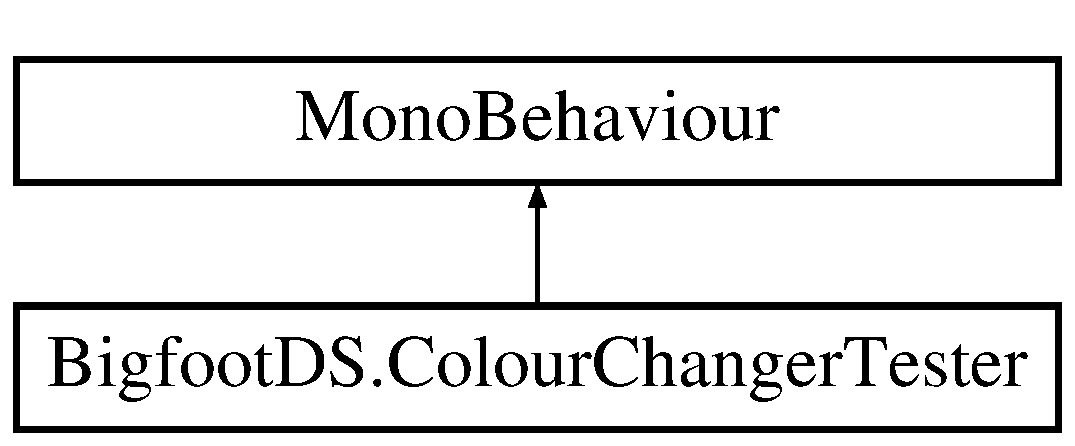
\includegraphics[height=2.000000cm]{class_bigfoot_d_s_1_1_colour_changer_tester}
\end{center}
\end{figure}
\subsection*{Public Member Functions}
\begin{DoxyCompactItemize}
\item 
void \mbox{\hyperlink{class_bigfoot_d_s_1_1_colour_changer_tester_a062a15842af6c9e67840e8827ea345ee}{Select\+Random\+Colour}} ()
\begin{DoxyCompactList}\small\item\em Selects a random colour from the appropriate \mbox{\hyperlink{class_singleton_scriptable_object}{Singleton\+Scriptable\+Object}} that contains references to web-\/friendly colours. \end{DoxyCompactList}\item 
void \mbox{\hyperlink{class_bigfoot_d_s_1_1_colour_changer_tester_a723b8d8bcccfccd194319e4ea608e821}{Colour\+Assigner}} ()
\begin{DoxyCompactList}\small\item\em Clamps the current\+Colour\+Index value to fit within an appropritate material list and then assigns that material to the object containing this script. \end{DoxyCompactList}\item 
void \mbox{\hyperlink{class_bigfoot_d_s_1_1_colour_changer_tester_af15ff93daa349ad267667db3f88f18c3}{Select\+Previous\+Colour}} ()
\begin{DoxyCompactList}\small\item\em Changes the colour index value and immediately calls the Colour\+Assigner function to change the colour of this object. \end{DoxyCompactList}\item 
void \mbox{\hyperlink{class_bigfoot_d_s_1_1_colour_changer_tester_ae480b9548f5407a651999676d1724da2}{Select\+Next\+Colour}} ()
\begin{DoxyCompactList}\small\item\em Changes the colour index value and immediately calls the Colour\+Assigner function to change the colour of this object. \end{DoxyCompactList}\end{DoxyCompactItemize}
\subsection*{Public Attributes}
\begin{DoxyCompactItemize}
\item 
\mbox{\hyperlink{namespace_bigfoot_d_s_abbe5e74a13ceee1200fe8df86775491b}{Colour\+Type}} \mbox{\hyperlink{class_bigfoot_d_s_1_1_colour_changer_tester_ab7fcdc500194580a3d2881be60ba2079}{this\+Colour\+Type}}
\begin{DoxyCompactList}\small\item\em The main colour types of the built-\/in web colour materials. Should be Default, Matte and Metallic! \end{DoxyCompactList}\item 
int \mbox{\hyperlink{class_bigfoot_d_s_1_1_colour_changer_tester_aa4dfb28508c536b6aeb95261415c64a6}{current\+Colour\+Index}} = 0
\begin{DoxyCompactList}\small\item\em Index value used to mark which current web colour material is in use. \end{DoxyCompactList}\item 
\mbox{\Hypertarget{class_bigfoot_d_s_1_1_colour_changer_tester_a7ac564ac5150e1cfadf622d9fc802e36}\label{class_bigfoot_d_s_1_1_colour_changer_tester_a7ac564ac5150e1cfadf622d9fc802e36}} 
string {\bfseries current\+Material\+Name}
\item 
\mbox{\Hypertarget{class_bigfoot_d_s_1_1_colour_changer_tester_a0dc48d1ef7ec4251172cd3a8f9469f7f}\label{class_bigfoot_d_s_1_1_colour_changer_tester_a0dc48d1ef7ec4251172cd3a8f9469f7f}} 
Text {\bfseries material\+Name\+Displayer}
\end{DoxyCompactItemize}


\subsection{Member Function Documentation}
\mbox{\Hypertarget{class_bigfoot_d_s_1_1_colour_changer_tester_a723b8d8bcccfccd194319e4ea608e821}\label{class_bigfoot_d_s_1_1_colour_changer_tester_a723b8d8bcccfccd194319e4ea608e821}} 
\index{Bigfoot\+D\+S\+::\+Colour\+Changer\+Tester@{Bigfoot\+D\+S\+::\+Colour\+Changer\+Tester}!Colour\+Assigner@{Colour\+Assigner}}
\index{Colour\+Assigner@{Colour\+Assigner}!Bigfoot\+D\+S\+::\+Colour\+Changer\+Tester@{Bigfoot\+D\+S\+::\+Colour\+Changer\+Tester}}
\subsubsection{\texorpdfstring{Colour\+Assigner()}{ColourAssigner()}}
{\footnotesize\ttfamily void Bigfoot\+D\+S.\+Colour\+Changer\+Tester.\+Colour\+Assigner (\begin{DoxyParamCaption}{ }\end{DoxyParamCaption})}



Clamps the current\+Colour\+Index value to fit within an appropritate material list and then assigns that material to the object containing this script. 

\mbox{\Hypertarget{class_bigfoot_d_s_1_1_colour_changer_tester_ae480b9548f5407a651999676d1724da2}\label{class_bigfoot_d_s_1_1_colour_changer_tester_ae480b9548f5407a651999676d1724da2}} 
\index{Bigfoot\+D\+S\+::\+Colour\+Changer\+Tester@{Bigfoot\+D\+S\+::\+Colour\+Changer\+Tester}!Select\+Next\+Colour@{Select\+Next\+Colour}}
\index{Select\+Next\+Colour@{Select\+Next\+Colour}!Bigfoot\+D\+S\+::\+Colour\+Changer\+Tester@{Bigfoot\+D\+S\+::\+Colour\+Changer\+Tester}}
\subsubsection{\texorpdfstring{Select\+Next\+Colour()}{SelectNextColour()}}
{\footnotesize\ttfamily void Bigfoot\+D\+S.\+Colour\+Changer\+Tester.\+Select\+Next\+Colour (\begin{DoxyParamCaption}{ }\end{DoxyParamCaption})}



Changes the colour index value and immediately calls the Colour\+Assigner function to change the colour of this object. 

\mbox{\Hypertarget{class_bigfoot_d_s_1_1_colour_changer_tester_af15ff93daa349ad267667db3f88f18c3}\label{class_bigfoot_d_s_1_1_colour_changer_tester_af15ff93daa349ad267667db3f88f18c3}} 
\index{Bigfoot\+D\+S\+::\+Colour\+Changer\+Tester@{Bigfoot\+D\+S\+::\+Colour\+Changer\+Tester}!Select\+Previous\+Colour@{Select\+Previous\+Colour}}
\index{Select\+Previous\+Colour@{Select\+Previous\+Colour}!Bigfoot\+D\+S\+::\+Colour\+Changer\+Tester@{Bigfoot\+D\+S\+::\+Colour\+Changer\+Tester}}
\subsubsection{\texorpdfstring{Select\+Previous\+Colour()}{SelectPreviousColour()}}
{\footnotesize\ttfamily void Bigfoot\+D\+S.\+Colour\+Changer\+Tester.\+Select\+Previous\+Colour (\begin{DoxyParamCaption}{ }\end{DoxyParamCaption})}



Changes the colour index value and immediately calls the Colour\+Assigner function to change the colour of this object. 

\mbox{\Hypertarget{class_bigfoot_d_s_1_1_colour_changer_tester_a062a15842af6c9e67840e8827ea345ee}\label{class_bigfoot_d_s_1_1_colour_changer_tester_a062a15842af6c9e67840e8827ea345ee}} 
\index{Bigfoot\+D\+S\+::\+Colour\+Changer\+Tester@{Bigfoot\+D\+S\+::\+Colour\+Changer\+Tester}!Select\+Random\+Colour@{Select\+Random\+Colour}}
\index{Select\+Random\+Colour@{Select\+Random\+Colour}!Bigfoot\+D\+S\+::\+Colour\+Changer\+Tester@{Bigfoot\+D\+S\+::\+Colour\+Changer\+Tester}}
\subsubsection{\texorpdfstring{Select\+Random\+Colour()}{SelectRandomColour()}}
{\footnotesize\ttfamily void Bigfoot\+D\+S.\+Colour\+Changer\+Tester.\+Select\+Random\+Colour (\begin{DoxyParamCaption}{ }\end{DoxyParamCaption})}



Selects a random colour from the appropriate \mbox{\hyperlink{class_singleton_scriptable_object}{Singleton\+Scriptable\+Object}} that contains references to web-\/friendly colours. 



\subsection{Member Data Documentation}
\mbox{\Hypertarget{class_bigfoot_d_s_1_1_colour_changer_tester_aa4dfb28508c536b6aeb95261415c64a6}\label{class_bigfoot_d_s_1_1_colour_changer_tester_aa4dfb28508c536b6aeb95261415c64a6}} 
\index{Bigfoot\+D\+S\+::\+Colour\+Changer\+Tester@{Bigfoot\+D\+S\+::\+Colour\+Changer\+Tester}!current\+Colour\+Index@{current\+Colour\+Index}}
\index{current\+Colour\+Index@{current\+Colour\+Index}!Bigfoot\+D\+S\+::\+Colour\+Changer\+Tester@{Bigfoot\+D\+S\+::\+Colour\+Changer\+Tester}}
\subsubsection{\texorpdfstring{current\+Colour\+Index}{currentColourIndex}}
{\footnotesize\ttfamily int Bigfoot\+D\+S.\+Colour\+Changer\+Tester.\+current\+Colour\+Index = 0}



Index value used to mark which current web colour material is in use. 

\mbox{\Hypertarget{class_bigfoot_d_s_1_1_colour_changer_tester_ab7fcdc500194580a3d2881be60ba2079}\label{class_bigfoot_d_s_1_1_colour_changer_tester_ab7fcdc500194580a3d2881be60ba2079}} 
\index{Bigfoot\+D\+S\+::\+Colour\+Changer\+Tester@{Bigfoot\+D\+S\+::\+Colour\+Changer\+Tester}!this\+Colour\+Type@{this\+Colour\+Type}}
\index{this\+Colour\+Type@{this\+Colour\+Type}!Bigfoot\+D\+S\+::\+Colour\+Changer\+Tester@{Bigfoot\+D\+S\+::\+Colour\+Changer\+Tester}}
\subsubsection{\texorpdfstring{this\+Colour\+Type}{thisColourType}}
{\footnotesize\ttfamily \mbox{\hyperlink{namespace_bigfoot_d_s_abbe5e74a13ceee1200fe8df86775491b}{Colour\+Type}} Bigfoot\+D\+S.\+Colour\+Changer\+Tester.\+this\+Colour\+Type}



The main colour types of the built-\/in web colour materials. Should be Default, Matte and Metallic! 



The documentation for this class was generated from the following file\+:\begin{DoxyCompactItemize}
\item 
Assets/\+Bigfoot\+D\+S/\+\_\+\+Common/\+Scripts/Colour\+Changer\+Tester.\+cs\end{DoxyCompactItemize}

\hypertarget{class_bigfoot_d_s_1_1_folder_structure_generator}{}\section{Bigfoot\+D\+S.\+Folder\+Structure\+Generator Class Reference}
\label{class_bigfoot_d_s_1_1_folder_structure_generator}\index{Bigfoot\+D\+S.\+Folder\+Structure\+Generator@{Bigfoot\+D\+S.\+Folder\+Structure\+Generator}}
Inheritance diagram for Bigfoot\+D\+S.\+Folder\+Structure\+Generator\+:\begin{figure}[H]
\begin{center}
\leavevmode
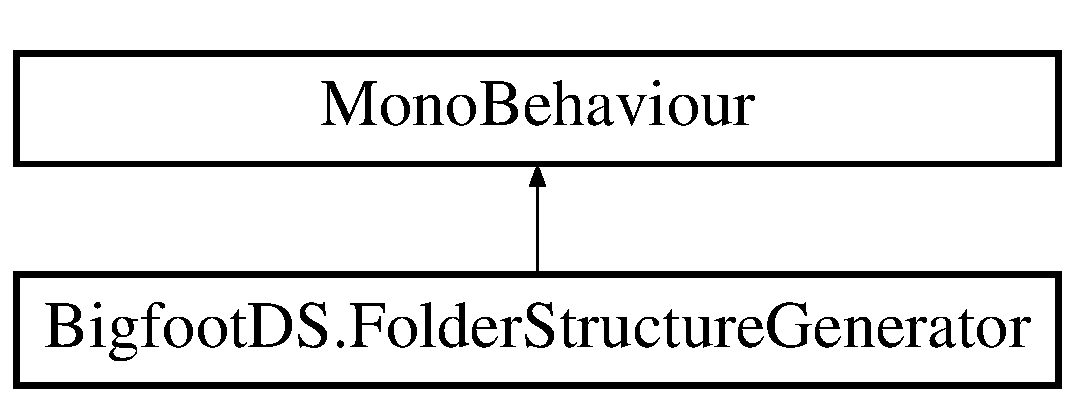
\includegraphics[height=2.000000cm]{class_bigfoot_d_s_1_1_folder_structure_generator}
\end{center}
\end{figure}
\subsection*{Static Public Member Functions}
\begin{DoxyCompactItemize}
\item 
\mbox{\Hypertarget{class_bigfoot_d_s_1_1_folder_structure_generator_aaddc799c445ab04cd16ff7386598e58d}\label{class_bigfoot_d_s_1_1_folder_structure_generator_aaddc799c445ab04cd16ff7386598e58d}} 
static void {\bfseries Generate\+Basic\+Folder\+Structure} ()
\end{DoxyCompactItemize}


The documentation for this class was generated from the following file\+:\begin{DoxyCompactItemize}
\item 
Assets/\+Bigfoot\+D\+S/\+\_\+\+Common/\+Scripts/\+Editor/Folder\+Structure\+Generator.\+cs\end{DoxyCompactItemize}

\hypertarget{class_bigfoot_d_s_1_1_folder_structure_wizard}{}\section{Bigfoot\+D\+S.\+Folder\+Structure\+Wizard Class Reference}
\label{class_bigfoot_d_s_1_1_folder_structure_wizard}\index{Bigfoot\+D\+S.\+Folder\+Structure\+Wizard@{Bigfoot\+D\+S.\+Folder\+Structure\+Wizard}}
Inheritance diagram for Bigfoot\+D\+S.\+Folder\+Structure\+Wizard\+:\begin{figure}[H]
\begin{center}
\leavevmode
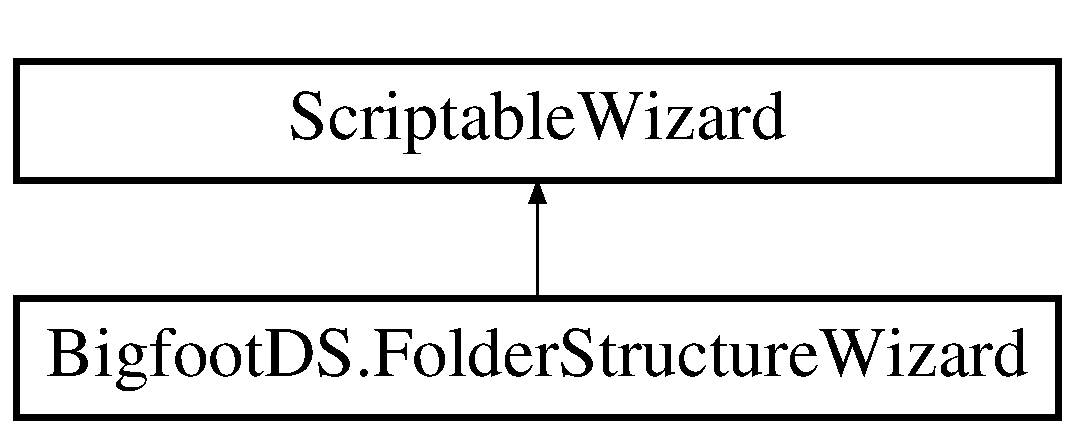
\includegraphics[height=2.000000cm]{class_bigfoot_d_s_1_1_folder_structure_wizard}
\end{center}
\end{figure}
\subsection*{Public Attributes}
\begin{DoxyCompactItemize}
\item 
\mbox{\Hypertarget{class_bigfoot_d_s_1_1_folder_structure_wizard_a50ea0ecdc934635b543b889f9b3a3137}\label{class_bigfoot_d_s_1_1_folder_structure_wizard_a50ea0ecdc934635b543b889f9b3a3137}} 
string {\bfseries folders\+Prefix} = \char`\"{}\char`\"{}
\item 
\mbox{\Hypertarget{class_bigfoot_d_s_1_1_folder_structure_wizard_a0d8cee92696e97b34af579efaae02ce6}\label{class_bigfoot_d_s_1_1_folder_structure_wizard_a0d8cee92696e97b34af579efaae02ce6}} 
string \mbox{[}$\,$\mbox{]} {\bfseries custom\+Folders\+To\+Generate} = new string\mbox{[}$\,$\mbox{]} \{ \char`\"{}\+\_\+\+\_\+\+Sandbox\char`\"{}, \char`\"{}\+\_\+\+Demo\char`\"{}, \char`\"{}\+\_\+\+Imported\+Assets\char`\"{}, \char`\"{}Animations\char`\"{}, \char`\"{}Audio\char`\"{}, \char`\"{}Fonts\char`\"{}, \char`\"{}Materials\char`\"{}, \char`\"{}Models\char`\"{}, \char`\"{}Prefabs\char`\"{}, \char`\"{}Plugins\char`\"{}, \char`\"{}Scriptable\+Objects\char`\"{}, \char`\"{}Scripts\char`\"{}, \char`\"{}Shaders\char`\"{}, \char`\"{}Sprites\char`\"{}, \char`\"{}Textures\char`\"{}, \char`\"{}Audio/S\+FX\char`\"{}, \char`\"{}Audio/Music\char`\"{}, \char`\"{}Scripts/Editor\char`\"{}, \char`\"{}Plugins/i\+OS\char`\"{}, \char`\"{}Plugins/Android\char`\"{} \}
\item 
\mbox{\Hypertarget{class_bigfoot_d_s_1_1_folder_structure_wizard_a1385e0b34ea11fe34b3fdd988f9e221d}\label{class_bigfoot_d_s_1_1_folder_structure_wizard_a1385e0b34ea11fe34b3fdd988f9e221d}} 
string \mbox{[}$\,$\mbox{]} {\bfseries backup\+Folders\+To\+Generate} = new string\mbox{[}0\mbox{]}
\end{DoxyCompactItemize}


The documentation for this class was generated from the following file\+:\begin{DoxyCompactItemize}
\item 
Assets/\+Bigfoot\+D\+S/\+\_\+\+Common/\+Scripts/\+Editor/Folder\+Structure\+Generator.\+cs\end{DoxyCompactItemize}

\hypertarget{class_bigfoot_d_s_1_1_scene_basics_generator}{}\section{Bigfoot\+D\+S.\+Scene\+Basics\+Generator Class Reference}
\label{class_bigfoot_d_s_1_1_scene_basics_generator}\index{Bigfoot\+D\+S.\+Scene\+Basics\+Generator@{Bigfoot\+D\+S.\+Scene\+Basics\+Generator}}
Inheritance diagram for Bigfoot\+D\+S.\+Scene\+Basics\+Generator\+:\begin{figure}[H]
\begin{center}
\leavevmode
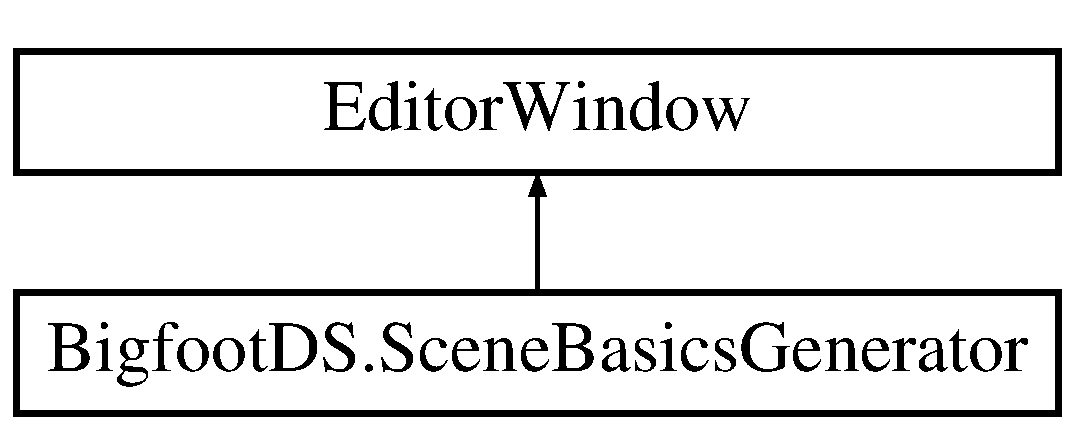
\includegraphics[height=2.000000cm]{class_bigfoot_d_s_1_1_scene_basics_generator}
\end{center}
\end{figure}
\subsection*{Static Public Member Functions}
\begin{DoxyCompactItemize}
\item 
\mbox{\Hypertarget{class_bigfoot_d_s_1_1_scene_basics_generator_a7658ebc40708b897c6f4685dcf4ec5f9}\label{class_bigfoot_d_s_1_1_scene_basics_generator_a7658ebc40708b897c6f4685dcf4ec5f9}} 
static void {\bfseries Show\+Window} ()
\end{DoxyCompactItemize}
\subsection*{Public Attributes}
\begin{DoxyCompactItemize}
\item 
\mbox{\Hypertarget{class_bigfoot_d_s_1_1_scene_basics_generator_a977290e611b430b3f8d18ad39dd2d63c}\label{class_bigfoot_d_s_1_1_scene_basics_generator_a977290e611b430b3f8d18ad39dd2d63c}} 
Game\+Object {\bfseries objects\+To\+Spawn}
\item 
\mbox{\Hypertarget{class_bigfoot_d_s_1_1_scene_basics_generator_aa1738e0af674139eb8956e3d4796c665}\label{class_bigfoot_d_s_1_1_scene_basics_generator_aa1738e0af674139eb8956e3d4796c665}} 
string {\bfseries ots\+Name} = \char`\"{}New Game\+Object\char`\"{}
\item 
\mbox{\Hypertarget{class_bigfoot_d_s_1_1_scene_basics_generator_a75a4abac9fa3686c027eae78527e880d}\label{class_bigfoot_d_s_1_1_scene_basics_generator_a75a4abac9fa3686c027eae78527e880d}} 
Vector3 {\bfseries ots\+Position}
\item 
\mbox{\Hypertarget{class_bigfoot_d_s_1_1_scene_basics_generator_af61d510b4d0620532443d89c21d96ebb}\label{class_bigfoot_d_s_1_1_scene_basics_generator_af61d510b4d0620532443d89c21d96ebb}} 
Vector3 {\bfseries ots\+Rotation}
\item 
\mbox{\Hypertarget{class_bigfoot_d_s_1_1_scene_basics_generator_a6fcfb33b239e0245687faaac690ccc66}\label{class_bigfoot_d_s_1_1_scene_basics_generator_a6fcfb33b239e0245687faaac690ccc66}} 
Vector3 {\bfseries ots\+Scale} = Vector3.\+one
\item 
\mbox{\Hypertarget{class_bigfoot_d_s_1_1_scene_basics_generator_a617e074c4a03c936ff9c8fc9110c1adc}\label{class_bigfoot_d_s_1_1_scene_basics_generator_a617e074c4a03c936ff9c8fc9110c1adc}} 
bool {\bfseries ots\+Static} = false
\end{DoxyCompactItemize}


The documentation for this class was generated from the following file\+:\begin{DoxyCompactItemize}
\item 
Assets/\+Bigfoot\+D\+S/\+\_\+\+Common/\+Scripts/\+Editor/Scene\+Basics\+Generator.\+cs\end{DoxyCompactItemize}

\hypertarget{class_bigfoot_d_s_1_1_scene_changing}{}\section{Bigfoot\+D\+S.\+Scene\+Changing Class Reference}
\label{class_bigfoot_d_s_1_1_scene_changing}\index{Bigfoot\+D\+S.\+Scene\+Changing@{Bigfoot\+D\+S.\+Scene\+Changing}}
Inheritance diagram for Bigfoot\+D\+S.\+Scene\+Changing\+:\begin{figure}[H]
\begin{center}
\leavevmode
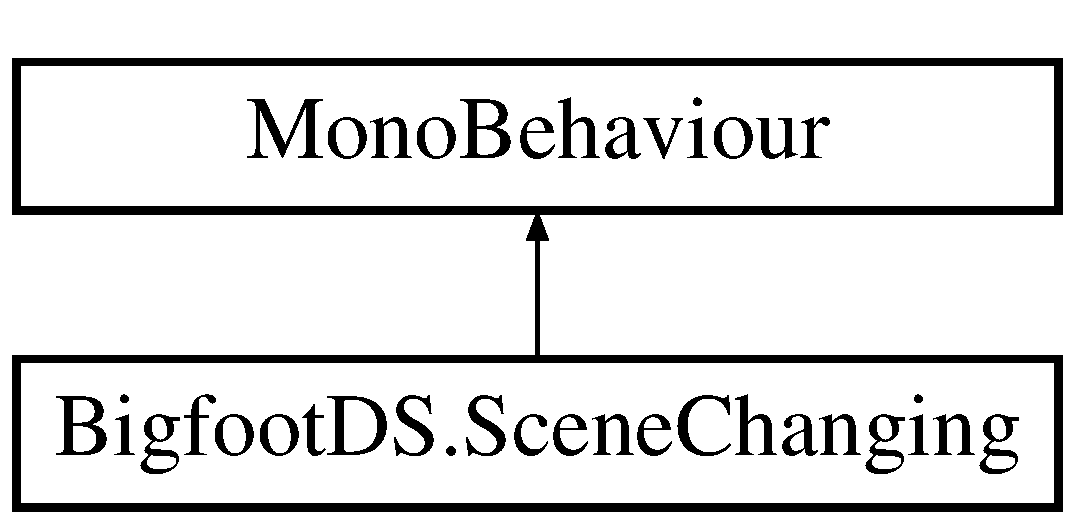
\includegraphics[height=2.000000cm]{class_bigfoot_d_s_1_1_scene_changing}
\end{center}
\end{figure}
\subsection*{Public Member Functions}
\begin{DoxyCompactItemize}
\item 
\mbox{\Hypertarget{class_bigfoot_d_s_1_1_scene_changing_a76bbba565a3d8b47978ce8df6a3fa982}\label{class_bigfoot_d_s_1_1_scene_changing_a76bbba565a3d8b47978ce8df6a3fa982}} 
void {\bfseries Change\+Scene\+No\+Sync} (int new\+Scene)
\item 
\mbox{\Hypertarget{class_bigfoot_d_s_1_1_scene_changing_a427180761a5ad002945c369f9120bfe9}\label{class_bigfoot_d_s_1_1_scene_changing_a427180761a5ad002945c369f9120bfe9}} 
void {\bfseries Change\+Scene\+A\+Sync} (int new\+Scene)
\item 
\mbox{\Hypertarget{class_bigfoot_d_s_1_1_scene_changing_a080d3784c25b537678b4962366f98413}\label{class_bigfoot_d_s_1_1_scene_changing_a080d3784c25b537678b4962366f98413}} 
void {\bfseries Next\+Scene\+No\+Sync} ()
\item 
\mbox{\Hypertarget{class_bigfoot_d_s_1_1_scene_changing_aec2e28e7f6ed45acbf39ebca6612f901}\label{class_bigfoot_d_s_1_1_scene_changing_aec2e28e7f6ed45acbf39ebca6612f901}} 
void {\bfseries Next\+Scene\+Async} ()
\item 
\mbox{\Hypertarget{class_bigfoot_d_s_1_1_scene_changing_a033c3a7a65174ef02075498d5e45ad7f}\label{class_bigfoot_d_s_1_1_scene_changing_a033c3a7a65174ef02075498d5e45ad7f}} 
void {\bfseries Previous\+Scene\+No\+Sync} ()
\item 
\mbox{\Hypertarget{class_bigfoot_d_s_1_1_scene_changing_a9f7e38dd6c634f1243aeccfe49710ba2}\label{class_bigfoot_d_s_1_1_scene_changing_a9f7e38dd6c634f1243aeccfe49710ba2}} 
void {\bfseries Previous\+Scene\+A\+Sync} ()
\end{DoxyCompactItemize}
\subsection*{Static Public Attributes}
\begin{DoxyCompactItemize}
\item 
\mbox{\Hypertarget{class_bigfoot_d_s_1_1_scene_changing_a646a0875eccb56b4f7cf8f62f541e554}\label{class_bigfoot_d_s_1_1_scene_changing_a646a0875eccb56b4f7cf8f62f541e554}} 
static \mbox{\hyperlink{class_bigfoot_d_s_1_1_scene_changing}{Scene\+Changing}} {\bfseries instance}
\end{DoxyCompactItemize}


The documentation for this class was generated from the following file\+:\begin{DoxyCompactItemize}
\item 
Assets/\+Bigfoot\+D\+S/\+\_\+\+Common/\+Scripts/Scene\+Changing.\+cs\end{DoxyCompactItemize}

\hypertarget{class_scene_view_actor_camera}{}\section{Scene\+View\+Actor\+Camera Class Reference}
\label{class_scene_view_actor_camera}\index{Scene\+View\+Actor\+Camera@{Scene\+View\+Actor\+Camera}}
Inheritance diagram for Scene\+View\+Actor\+Camera\+:\begin{figure}[H]
\begin{center}
\leavevmode
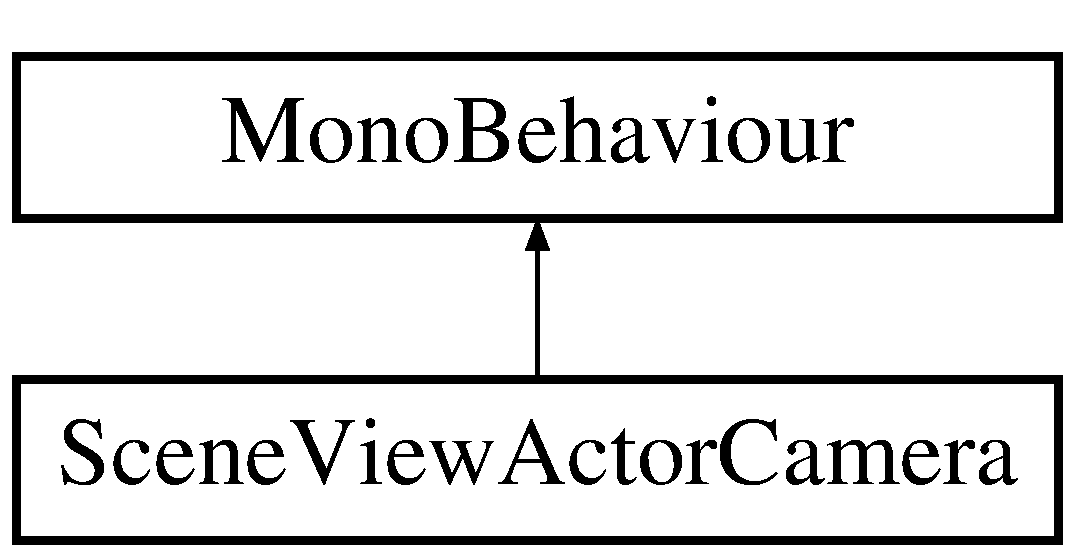
\includegraphics[height=2.000000cm]{class_scene_view_actor_camera}
\end{center}
\end{figure}
\subsection*{Static Public Member Functions}
\begin{DoxyCompactItemize}
\item 
\mbox{\Hypertarget{class_scene_view_actor_camera_a99fc940c929ecd0be983f6d5f606c7df}\label{class_scene_view_actor_camera_a99fc940c929ecd0be983f6d5f606c7df}} 
static void {\bfseries Quick\+Move\+Main\+Cam\+To\+Scene\+Cam} ()
\item 
\mbox{\Hypertarget{class_scene_view_actor_camera_a2c008ee53d553b0ff4ed85f5c02e8319}\label{class_scene_view_actor_camera_a2c008ee53d553b0ff4ed85f5c02e8319}} 
static void {\bfseries Reset\+Main\+Cam\+To\+World\+Zero} ()
\item 
\mbox{\Hypertarget{class_scene_view_actor_camera_a64bdb8bab8474234aa7d7feaca807eee}\label{class_scene_view_actor_camera_a64bdb8bab8474234aa7d7feaca807eee}} 
static void {\bfseries Reset\+Main\+Cam\+To\+Unity\+Default} ()
\item 
static void \mbox{\hyperlink{class_scene_view_actor_camera_a3e544b9e43a8dba5304140b3661752b1}{Match\+Main\+Camera\+To\+Values}} ()
\begin{DoxyCompactList}\small\item\em This overload will force the Main Camera to match the Scene View camera. \end{DoxyCompactList}\item 
static void \mbox{\hyperlink{class_scene_view_actor_camera_a77349efed7b218f0c931926186cecd4e}{Match\+Main\+Camera\+To\+Values}} (Vector3 new\+Position, Quaternion new\+Rotation, Vector3 new\+Scale, bool use\+Global\+Space)
\begin{DoxyCompactList}\small\item\em Make the scene\textquotesingle{}s Main Camera move to specified values. This overload lets you specify every value, and takes in the rotation values as a Quaternion instead of a Vector3. \end{DoxyCompactList}\item 
static void \mbox{\hyperlink{class_scene_view_actor_camera_aceebf34bad9730f98c6e04fc264883be}{Match\+Main\+Camera\+To\+Values}} (Vector3 new\+Position, Quaternion new\+Rotation, Vector3 new\+Scale)
\begin{DoxyCompactList}\small\item\em Make the scene\textquotesingle{}s Main Camera move to specified values. This overload lets you specify every value, and takes in the rotation values as a Vector3 instead of a Quaternion. Defaults to modifying position \& rotation in worldspace. \end{DoxyCompactList}\item 
static void \mbox{\hyperlink{class_scene_view_actor_camera_ae248bbbefe424aabc56875b4f7bf942d}{Match\+Main\+Camera\+To\+Values}} (Vector3 new\+Position, Vector3 new\+Rotation, Vector3 new\+Scale, bool use\+Global\+Space)
\begin{DoxyCompactList}\small\item\em Make the scene\textquotesingle{}s Main Camera move to specified values. This overload lets you specify every value, and takes in the rotation values as a Vector3 instead of a Quaternion. \end{DoxyCompactList}\item 
static void \mbox{\hyperlink{class_scene_view_actor_camera_a66ac86cd938970082513231063316872}{Match\+Main\+Camera\+To\+Values}} (Vector3 new\+Position, Vector3 new\+Rotation, Vector3 new\+Scale)
\begin{DoxyCompactList}\small\item\em Make the scene\textquotesingle{}s Main Camera move to specified values. This overload lets you specify every value, and takes in the rotation values as a Vector3 instead of a Quaternion. Defaults to modifying position \& rotation in worldspace. \end{DoxyCompactList}\item 
static void \mbox{\hyperlink{class_scene_view_actor_camera_a6803c2185afa5fb555dd64eafdab31b6}{Match\+Main\+Camera\+To\+Values}} (bool zero\+The\+Camera, bool reset\+To\+Unity\+Default)
\begin{DoxyCompactList}\small\item\em Make the scene\textquotesingle{}s Main Camera move to specified values. This overload will let you choose between one of two options\+: either reset the Main Camera to the world-\/zero, or reset it to Unity\textquotesingle{}s default values. This overload will fail if both are true or if both are false. \end{DoxyCompactList}\end{DoxyCompactItemize}
\subsection*{Properties}
\begin{DoxyCompactItemize}
\item 
\mbox{\Hypertarget{class_scene_view_actor_camera_a0de0dd5d70d8e78328be80c326882725}\label{class_scene_view_actor_camera_a0de0dd5d70d8e78328be80c326882725}} 
static bool {\bfseries Is\+Actor\+Cam\+Enabled}\hspace{0.3cm}{\ttfamily  \mbox{[}get, set\mbox{]}}
\end{DoxyCompactItemize}


\subsection{Member Function Documentation}
\mbox{\Hypertarget{class_scene_view_actor_camera_a3e544b9e43a8dba5304140b3661752b1}\label{class_scene_view_actor_camera_a3e544b9e43a8dba5304140b3661752b1}} 
\index{Scene\+View\+Actor\+Camera@{Scene\+View\+Actor\+Camera}!Match\+Main\+Camera\+To\+Values@{Match\+Main\+Camera\+To\+Values}}
\index{Match\+Main\+Camera\+To\+Values@{Match\+Main\+Camera\+To\+Values}!Scene\+View\+Actor\+Camera@{Scene\+View\+Actor\+Camera}}
\subsubsection{\texorpdfstring{Match\+Main\+Camera\+To\+Values()}{MatchMainCameraToValues()}\hspace{0.1cm}{\footnotesize\ttfamily [1/6]}}
{\footnotesize\ttfamily static void Scene\+View\+Actor\+Camera.\+Match\+Main\+Camera\+To\+Values (\begin{DoxyParamCaption}{ }\end{DoxyParamCaption})\hspace{0.3cm}{\ttfamily [static]}}



This overload will force the Main Camera to match the Scene View camera. 

\mbox{\Hypertarget{class_scene_view_actor_camera_a77349efed7b218f0c931926186cecd4e}\label{class_scene_view_actor_camera_a77349efed7b218f0c931926186cecd4e}} 
\index{Scene\+View\+Actor\+Camera@{Scene\+View\+Actor\+Camera}!Match\+Main\+Camera\+To\+Values@{Match\+Main\+Camera\+To\+Values}}
\index{Match\+Main\+Camera\+To\+Values@{Match\+Main\+Camera\+To\+Values}!Scene\+View\+Actor\+Camera@{Scene\+View\+Actor\+Camera}}
\subsubsection{\texorpdfstring{Match\+Main\+Camera\+To\+Values()}{MatchMainCameraToValues()}\hspace{0.1cm}{\footnotesize\ttfamily [2/6]}}
{\footnotesize\ttfamily static void Scene\+View\+Actor\+Camera.\+Match\+Main\+Camera\+To\+Values (\begin{DoxyParamCaption}\item[{Vector3}]{new\+Position,  }\item[{Quaternion}]{new\+Rotation,  }\item[{Vector3}]{new\+Scale,  }\item[{bool}]{use\+Global\+Space }\end{DoxyParamCaption})\hspace{0.3cm}{\ttfamily [static]}}



Make the scene\textquotesingle{}s Main Camera move to specified values. This overload lets you specify every value, and takes in the rotation values as a Quaternion instead of a Vector3. 


\begin{DoxyParams}{Parameters}
{\em new\+Position} & New position coordinates.\\
\hline
{\em new\+Rotation} & New rotation values\\
\hline
{\em new\+Scale} & New scale multiplier values.\\
\hline
{\em use\+Global\+Space} & If this is true, all values above will be applied in world/global space.\\
\hline
\end{DoxyParams}
\mbox{\Hypertarget{class_scene_view_actor_camera_aceebf34bad9730f98c6e04fc264883be}\label{class_scene_view_actor_camera_aceebf34bad9730f98c6e04fc264883be}} 
\index{Scene\+View\+Actor\+Camera@{Scene\+View\+Actor\+Camera}!Match\+Main\+Camera\+To\+Values@{Match\+Main\+Camera\+To\+Values}}
\index{Match\+Main\+Camera\+To\+Values@{Match\+Main\+Camera\+To\+Values}!Scene\+View\+Actor\+Camera@{Scene\+View\+Actor\+Camera}}
\subsubsection{\texorpdfstring{Match\+Main\+Camera\+To\+Values()}{MatchMainCameraToValues()}\hspace{0.1cm}{\footnotesize\ttfamily [3/6]}}
{\footnotesize\ttfamily static void Scene\+View\+Actor\+Camera.\+Match\+Main\+Camera\+To\+Values (\begin{DoxyParamCaption}\item[{Vector3}]{new\+Position,  }\item[{Quaternion}]{new\+Rotation,  }\item[{Vector3}]{new\+Scale }\end{DoxyParamCaption})\hspace{0.3cm}{\ttfamily [static]}}



Make the scene\textquotesingle{}s Main Camera move to specified values. This overload lets you specify every value, and takes in the rotation values as a Vector3 instead of a Quaternion. Defaults to modifying position \& rotation in worldspace. 


\begin{DoxyParams}{Parameters}
{\em new\+Position} & New position coordinates.\\
\hline
{\em new\+Rotation} & New rotation values\\
\hline
{\em new\+Scale} & New scale multiplier values.\\
\hline
\end{DoxyParams}
\mbox{\Hypertarget{class_scene_view_actor_camera_ae248bbbefe424aabc56875b4f7bf942d}\label{class_scene_view_actor_camera_ae248bbbefe424aabc56875b4f7bf942d}} 
\index{Scene\+View\+Actor\+Camera@{Scene\+View\+Actor\+Camera}!Match\+Main\+Camera\+To\+Values@{Match\+Main\+Camera\+To\+Values}}
\index{Match\+Main\+Camera\+To\+Values@{Match\+Main\+Camera\+To\+Values}!Scene\+View\+Actor\+Camera@{Scene\+View\+Actor\+Camera}}
\subsubsection{\texorpdfstring{Match\+Main\+Camera\+To\+Values()}{MatchMainCameraToValues()}\hspace{0.1cm}{\footnotesize\ttfamily [4/6]}}
{\footnotesize\ttfamily static void Scene\+View\+Actor\+Camera.\+Match\+Main\+Camera\+To\+Values (\begin{DoxyParamCaption}\item[{Vector3}]{new\+Position,  }\item[{Vector3}]{new\+Rotation,  }\item[{Vector3}]{new\+Scale,  }\item[{bool}]{use\+Global\+Space }\end{DoxyParamCaption})\hspace{0.3cm}{\ttfamily [static]}}



Make the scene\textquotesingle{}s Main Camera move to specified values. This overload lets you specify every value, and takes in the rotation values as a Vector3 instead of a Quaternion. 


\begin{DoxyParams}{Parameters}
{\em new\+Position} & New position coordinates.\\
\hline
{\em new\+Rotation} & New rotation values\\
\hline
{\em new\+Scale} & New scale multiplier values.\\
\hline
{\em use\+Global\+Space} & If this is true, all values above will be applied in world/global space.\\
\hline
\end{DoxyParams}
\mbox{\Hypertarget{class_scene_view_actor_camera_a66ac86cd938970082513231063316872}\label{class_scene_view_actor_camera_a66ac86cd938970082513231063316872}} 
\index{Scene\+View\+Actor\+Camera@{Scene\+View\+Actor\+Camera}!Match\+Main\+Camera\+To\+Values@{Match\+Main\+Camera\+To\+Values}}
\index{Match\+Main\+Camera\+To\+Values@{Match\+Main\+Camera\+To\+Values}!Scene\+View\+Actor\+Camera@{Scene\+View\+Actor\+Camera}}
\subsubsection{\texorpdfstring{Match\+Main\+Camera\+To\+Values()}{MatchMainCameraToValues()}\hspace{0.1cm}{\footnotesize\ttfamily [5/6]}}
{\footnotesize\ttfamily static void Scene\+View\+Actor\+Camera.\+Match\+Main\+Camera\+To\+Values (\begin{DoxyParamCaption}\item[{Vector3}]{new\+Position,  }\item[{Vector3}]{new\+Rotation,  }\item[{Vector3}]{new\+Scale }\end{DoxyParamCaption})\hspace{0.3cm}{\ttfamily [static]}}



Make the scene\textquotesingle{}s Main Camera move to specified values. This overload lets you specify every value, and takes in the rotation values as a Vector3 instead of a Quaternion. Defaults to modifying position \& rotation in worldspace. 


\begin{DoxyParams}{Parameters}
{\em new\+Position} & New position coordinates.\\
\hline
{\em new\+Rotation} & New rotation values\\
\hline
{\em new\+Scale} & New scale multiplier values.\\
\hline
{\em use\+Global\+Space} & If this is true, all values above will be applied in world/global space.\\
\hline
\end{DoxyParams}
\mbox{\Hypertarget{class_scene_view_actor_camera_a6803c2185afa5fb555dd64eafdab31b6}\label{class_scene_view_actor_camera_a6803c2185afa5fb555dd64eafdab31b6}} 
\index{Scene\+View\+Actor\+Camera@{Scene\+View\+Actor\+Camera}!Match\+Main\+Camera\+To\+Values@{Match\+Main\+Camera\+To\+Values}}
\index{Match\+Main\+Camera\+To\+Values@{Match\+Main\+Camera\+To\+Values}!Scene\+View\+Actor\+Camera@{Scene\+View\+Actor\+Camera}}
\subsubsection{\texorpdfstring{Match\+Main\+Camera\+To\+Values()}{MatchMainCameraToValues()}\hspace{0.1cm}{\footnotesize\ttfamily [6/6]}}
{\footnotesize\ttfamily static void Scene\+View\+Actor\+Camera.\+Match\+Main\+Camera\+To\+Values (\begin{DoxyParamCaption}\item[{bool}]{zero\+The\+Camera,  }\item[{bool}]{reset\+To\+Unity\+Default }\end{DoxyParamCaption})\hspace{0.3cm}{\ttfamily [static]}}



Make the scene\textquotesingle{}s Main Camera move to specified values. This overload will let you choose between one of two options\+: either reset the Main Camera to the world-\/zero, or reset it to Unity\textquotesingle{}s default values. This overload will fail if both are true or if both are false. 


\begin{DoxyParams}{Parameters}
{\em zero\+The\+Camera} & Reset the Main Camera\textquotesingle{}s position \& rotation to Vector3.\+zero, and scale of Vector3.\+one.\\
\hline
{\em reset\+To\+Unity\+Default} & Reset the Main Camera\textquotesingle{}s position to X0, Y1, Z-\/10, rotation to Vector3.\+zero, and scale to Vector3.\+one.\\
\hline
\end{DoxyParams}


The documentation for this class was generated from the following file\+:\begin{DoxyCompactItemize}
\item 
Assets/\+Bigfoot\+D\+S/\+\_\+\+Common/\+Scripts/\+Editor/Scene\+View\+Actor\+Camera.\+cs\end{DoxyCompactItemize}

\hypertarget{class_bigfoot_d_s_1_1_simple_point_to_point_mover}{}\section{Bigfoot\+D\+S.\+Simple\+Point\+To\+Point\+Mover Class Reference}
\label{class_bigfoot_d_s_1_1_simple_point_to_point_mover}\index{Bigfoot\+D\+S.\+Simple\+Point\+To\+Point\+Mover@{Bigfoot\+D\+S.\+Simple\+Point\+To\+Point\+Mover}}
Inheritance diagram for Bigfoot\+D\+S.\+Simple\+Point\+To\+Point\+Mover\+:\begin{figure}[H]
\begin{center}
\leavevmode
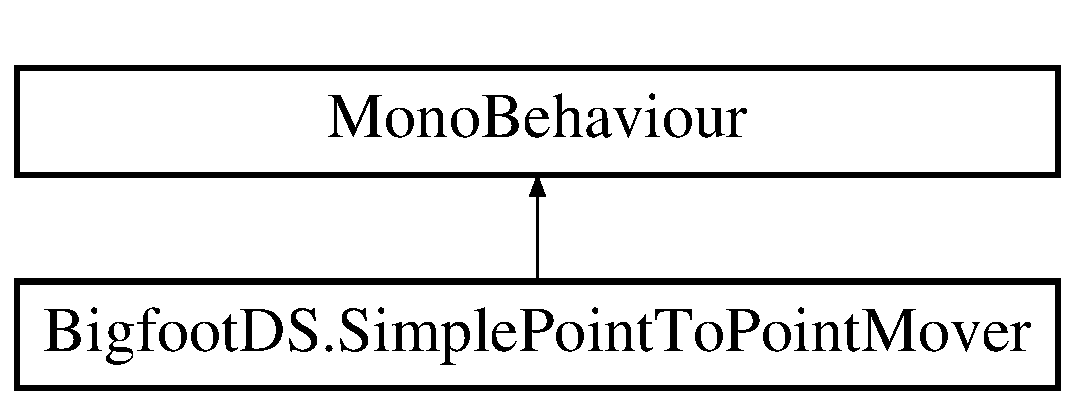
\includegraphics[height=2.000000cm]{class_bigfoot_d_s_1_1_simple_point_to_point_mover}
\end{center}
\end{figure}
\subsection*{Public Attributes}
\begin{DoxyCompactItemize}
\item 
\mbox{\Hypertarget{class_bigfoot_d_s_1_1_simple_point_to_point_mover_af03dba084f0e3c2cad7041ac22e7df66}\label{class_bigfoot_d_s_1_1_simple_point_to_point_mover_af03dba084f0e3c2cad7041ac22e7df66}} 
float {\bfseries destination\+Stop\+Delay} = 1
\item 
\mbox{\Hypertarget{class_bigfoot_d_s_1_1_simple_point_to_point_mover_a6e5600a3333bce2d0a75aa34e5eb4a85}\label{class_bigfoot_d_s_1_1_simple_point_to_point_mover_a6e5600a3333bce2d0a75aa34e5eb4a85}} 
float {\bfseries destination\+Distance\+Offset} = 0.\+5f
\item 
\mbox{\Hypertarget{class_bigfoot_d_s_1_1_simple_point_to_point_mover_a00fcff6e73f20c51bc8c2e627e25ef9d}\label{class_bigfoot_d_s_1_1_simple_point_to_point_mover_a00fcff6e73f20c51bc8c2e627e25ef9d}} 
Transform \mbox{[}$\,$\mbox{]} {\bfseries points\+To\+Move\+Between}
\item 
\mbox{\Hypertarget{class_bigfoot_d_s_1_1_simple_point_to_point_mover_a5d4418a9afe7800e8ed81457a825b00d}\label{class_bigfoot_d_s_1_1_simple_point_to_point_mover_a5d4418a9afe7800e8ed81457a825b00d}} 
float {\bfseries movement\+Speed} = 5
\item 
\mbox{\Hypertarget{class_bigfoot_d_s_1_1_simple_point_to_point_mover_ae41af53fb5b5c4416ea14fae42db521b}\label{class_bigfoot_d_s_1_1_simple_point_to_point_mover_ae41af53fb5b5c4416ea14fae42db521b}} 
bool {\bfseries is\+Stopped} = false
\end{DoxyCompactItemize}


The documentation for this class was generated from the following file\+:\begin{DoxyCompactItemize}
\item 
Assets/\+Bigfoot\+D\+S/\+\_\+\+Common/\+Scripts/Simple\+Point\+To\+Point\+Mover.\+cs\end{DoxyCompactItemize}

\hypertarget{class_singleton_scriptable_object}{}\section{Singleton\+Scriptable\+Object$<$ T $>$ Class Template Reference}
\label{class_singleton_scriptable_object}\index{Singleton\+Scriptable\+Object$<$ T $>$@{Singleton\+Scriptable\+Object$<$ T $>$}}
Inheritance diagram for Singleton\+Scriptable\+Object$<$ T $>$\+:\begin{figure}[H]
\begin{center}
\leavevmode
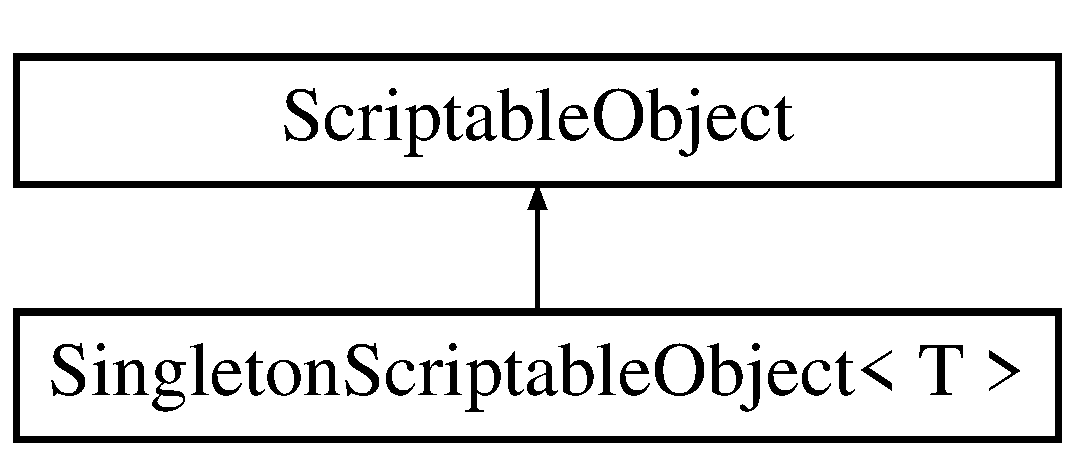
\includegraphics[height=2.000000cm]{class_singleton_scriptable_object}
\end{center}
\end{figure}
\subsection*{Properties}
\begin{DoxyCompactItemize}
\item 
\mbox{\Hypertarget{class_singleton_scriptable_object_ab7d1b120991063507e31e1925880ac43}\label{class_singleton_scriptable_object_ab7d1b120991063507e31e1925880ac43}} 
static T {\bfseries data}\hspace{0.3cm}{\ttfamily  \mbox{[}get\mbox{]}}
\end{DoxyCompactItemize}


The documentation for this class was generated from the following file\+:\begin{DoxyCompactItemize}
\item 
Assets/\+Bigfoot\+D\+S/\+\_\+\+Common/\+Scripts/Singleton\+Scriptable\+Object.\+cs\end{DoxyCompactItemize}

\hypertarget{class_bigfoot_d_s_1_1_bigfoot_event_invoker_1_1_specified_event}{}\section{Bigfoot\+D\+S.\+Bigfoot\+Event\+Invoker.\+Specified\+Event Class Reference}
\label{class_bigfoot_d_s_1_1_bigfoot_event_invoker_1_1_specified_event}\index{Bigfoot\+D\+S.\+Bigfoot\+Event\+Invoker.\+Specified\+Event@{Bigfoot\+D\+S.\+Bigfoot\+Event\+Invoker.\+Specified\+Event}}
Inheritance diagram for Bigfoot\+D\+S.\+Bigfoot\+Event\+Invoker.\+Specified\+Event\+:\begin{figure}[H]
\begin{center}
\leavevmode
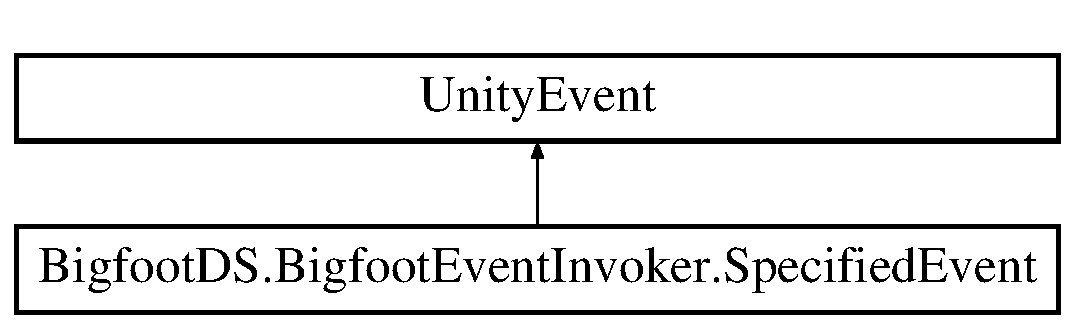
\includegraphics[height=2.000000cm]{class_bigfoot_d_s_1_1_bigfoot_event_invoker_1_1_specified_event}
\end{center}
\end{figure}


The documentation for this class was generated from the following file\+:\begin{DoxyCompactItemize}
\item 
Assets/\+Bigfoot\+D\+S/\+\_\+\+Common/\+Scripts/Bigfoot\+Event\+Invoker.\+cs\end{DoxyCompactItemize}

%--- End generated contents ---

% Index
\backmatter
\newpage
\phantomsection
\clearemptydoublepage
\addcontentsline{toc}{chapter}{Index}
\printindex

\end{document}
